\chapter{Energy Estimators}
\label{chap:energyestimators}

\chapterquote{There, sir! that is the perfection of vessels!}
{Jules Verne, 1828--1905}

%========================================================================================
%========================================================================================

\section{Motivation}
\label{sec:motivation}
% Results use detector model 85 and calibration variant 71
The separation of energy deposits from charged and neutral particles in the calorimeters is crucial for achieving good energy resolutions in the particle flow paradigm.  This is only possible if the energy estimators for those energy deposits are accurate.  The ultimate goal of the calibration procedure outlined in this chapter is to obtain the best energy estimator for particles showering in the calorimeters.  The energy estimator for a cluster of calorimeter hits is:
%
\begin{equation}
E_{Cluster} & = \sum_{ECal \text{ } hits \text{, }i} E^{i}_{ECal} +\sum_{HCal \text{ } hits \text{, }i} E^{i}_{HCal} \text{ ,}
\end{equation}
%
\noindent where $E^{i}_{ECal}$ is the energy of ECal hit $i$, $E^{i}_{HCal}$ is the energy HCal hit $i$ and $\sum$ is the summation over all hits in a given calorimeter.  This is a naive energy estimator that will act as a starting point for the development of more sophisticated procedures aimed at improving detector performance.  However, before going further the calorimeter hit energies must be determined, which for a sampling calorimeter is non-trivial.  Sampling calorimeters, such as those found at the linear collider, are comprised of alternating layers of active and absorber materials \cite{Fabjan:2003aq};  The absorber layers are designed to initiate particle showers and propagate their development, while the active layers are designed to give a response that is proportional to the energy deposited within them.  As the response of a sampling calorimeter gives a measure of the energy deposited in the active layers only, the energy deposited in the absorber medium has to be estimated based on the active layer energies.  This estimation is made by assuming the energy deposited across a calorimeter hit, that is one active and one absorber layer, is uniform.  Working under this assumption, the total calorimeter hit energy is proportional to the active layer hit energy.  This estimation procedure is loosely referred to as digitisation and, in this way, the cluster energy estimator introduced above can be written as:
%
\begin{equation}
E_{Cluster} = \sum_{ECal \text{ } hits \text{, }i} \epsilon^{i}_{ECal} \alpha_{ECal} + \sum_{HCal \text{ } hits \text{, }i} \epsilon^{i}_{HCal} \alpha_{HCal} \text{ ,}
\end{equation}
%
\noindent where \alpha_{ECal} and \alpha_{HCal} are digitisation constants for the ECal and HCal respectively, $\epsilon^{i}_{ECal}$ is the energy response in the active medium for ECal hit $i$, $\epsilon^{i}_{HCal}$ is the energy response in the active medium for a HCal hit $i$ and $\sum$ is the summation over all hits in a given calorimeter.  The first stage of the calibration procedure presented in this chapter covers the determination of these digitisation constants.  

Once the basic energy estimator has been calibrated, it is possible to apply more advanced procedures designed to give a compensating calorimeter response.  A compensating calorimeter produces an identical response to a particle shower irrespective of whether the particle shower is electromagnetic or hadronic in nature.  It is the atomic properties of the materials used in a calorimeter that determine whether a calorimeter is compensating.  The primary cause of a difference in the response of a calorimeter to electromagnetic and hadronic showers is the invisible energy component that is found in hadronic showers.  As this component cannot be measured by the calorimeter, the response is typically lower for hadronically showering particles than for electromagnetically showering particles.  The invisible component exists due to a combination of effects such as neutrons stopping within the calorimeter and nuclear binding energy losses.  If left unchecked, this difference would lead to a systematic loss of energy for hadronic showers that would harm detector performance.  

There are two distinct routes available for negating this unwanted effect and achieving a compensating response from a calorimeter:  The first is hardware compensation, whereby calorimeters are constructed using materials that yield extra energy in response to hadronic showers, and the second is software compensation, whereby the uncompensated calorimetric energies for hadronic showers are modified at the software level.  The linear collider lends itself to software compensation as the fine segmentation of the calorimeters and precise reconstruction of individual particles makes identification of hadronic showers, and modifying their energies, feasible.  A basic form of software compensation included in the linear collider reconstruction is the modification of the electromagnetic cluster energy estimator to:
%
\begin{equation}
E_{EM \text{ } Cluster} & = \sum_{ECal \text{ } hits \text{, }i} E^{i}_{ECal} \beta^{EM}_{ECal} + \sum_{HCal \text{ } hits \text{, }i} E^{i}_{HCal} \beta^{EM}_{HCal} \text{ ,}
\end{equation}
%
\noindent and the hadronic cluster energy to:
%
\begin{equation}
E_{Had \text{ } Cluster} & = \sum_{ECal \text{ } hits \text{, }i} E^{i}_{ECal} \beta^{Had}_{ECal} + \sum_{HCal \text{ } hits \text{, }i} E^{i}_{HCal} \beta^{Had}_{HCal} \text{ ,}
\end{equation}
%
\noindent where the $\beta$s are scaling factors that are applied to the energy of clusters of calorimeter hits associated with electromagnetic and hadronic clusters in the ECal and HCal.  This simple scaling of energies compensates the response of the calorimeters, which leads to better detector performance.  Determination of these energy scale setting constants is the second stage of the calibration procedure that is presented in this chapter.  

While this scaling of energies improves detector performance, it does not account for any changes to the $\beta$ scaling factors as a function of the total energy deposited.  An energy dependence in the scaling factors is expected as the mechanisms governing the propagation of hadronic showers are sensitive to the shower energy \cite{Wigmans:2000vf}.  To account for this, more sophisticated software techniques have been developed that vary the calorimeter cluster energy estimator as a function of energy to achieve a compensating response across a wider range of energies.  These techniques make use of the fine segmentation of the linear collider calorimeters to identify hadronic showers.  These techniques also address the problem of spuriously high energy calorimeter hits that if left unchecked would damage the reconstruction.  These high energy hits are caused by Landau fluctuations \cite{Landau:1944if}, which originate from high energy knock-on electrons appearing within particle showers \cite{Bichsel:2004ej}.  In this chapter, following a description of the calibration procedure outlined above, is an explanation of these novel energy estimators and the impact they have on detector performance.  

This chapter concludes with a study determining the impact on detector performance of timing cuts that are applied to the calorimeter hits.  These cuts form part of the software trigger that will be used at the linear collider experiment.  Details regarding how all the detector performance metrics used in this chapter are calculated can be found in section \ref{sec:optstudiesmetric}.

%========================================================================================

\subsubsection{Hardware Compensation}
A novel example of hardware compensation is the ZEUS calorimeter \cite{Derrick:1991tq}.  The ZEUS calorimeter was constructed using uranium as the absorber material.  In response to neutral hadrons the uranium undergoes fission producing extra energy that increases the hadronic response of the calorimeter.  The amount of uranium was carefully chosen to achieve a fully compensating calorimeter response i.e. identical calorimeter response to electromagnetic and hadronic showers.  While hardware compensation is possible for the linear collider calorimeters, restrictions on calorimeter construction and the use of a large amount of radioactive material are highly undesirable.  

%========================================================================================

\subsubsection{Calibration and detector optimisation}
Optimising the detector at a future linear collider will be crucial to exploit the full physics potential available to it.  An extensive optimisation of the calorimeters was performed and the results can be found in chapter \ref{sec:optimisationstudies}.  For each detector model considered, the calibration procedure outlined in section \ref{sec:overviewcalibration} was applied to ensure optimal energy estimators were used to quantify the detector performance.  This made it possible to perform unbiased comparisons between detector models, which ensured reliability in the conclusions drawn from those studies.

%========================================================================================

\section{Calibration in the particle flow paradigm}
\label{sec:overviewcalibration}
The calibration procedure described in the following section discusses how the digitisation constants, $\alpha$, and the scaling factors $\beta$ introduced in section \ref{sec:motivation} are determined.  In addition, two further operations are included in the general calibration procedure designed to ensure optimal detector performance.  These are minimum ionising particle (MIP) scale setting and retraining of likelihood data used in the reconstruction.  

The MIP scale is the average energy response, on a per hit level, of a calorimeter when a normally incident MIP passes through it.  This scale must be set in the digitisation processor as the response of the readout technology is simulated in this processor, which includes a maximum readout value set in units of MIPs.  The digitiser also applies a minimum threshold on the active layer hit energy, in units of MIPs, for calorimeter hit to be created.  PandoraPFA uses the MIP scale to place further threshold cuts on the hit energy that must be exceeded for a calorimeter hit to be used in the reconstruction.  Both of these thresholds are designed to veto noise that would be present in a real detector.  Although noise is not applied in any simulations presented in this work, these cuts are applied to better reflect the performance of a real detector.  The MIP scale in the digitiser and PandoraPFA, while intrinsically linked, have to be calculated separately as the digitiser requires the MIP scale to be defined using the active layer hit energies while, PandoraPFA requires the definition from the full hit, the active and absorber layer, energies.  It may be expected that the digitisation MIP scale could be related to the PandoraPFA MIP scale by the digitisation constants, however, this is not necessarily the case as additional cuts are applied to the full calorimeter hit energies that are not applied to the active layer hit energies e.g. timing cuts.  Therefore, the conservative approach of independently recalculating the MIP scale for PandoraPFA was taken.   

The likelihood data that is used in the reconstruction consists of a series of probability density functions (PDFs), which describe a number of topological properties of clusters of calorimeter hits.  This data is used to determine whether a cluster of hits corresponds to an electromagnetically showering particle.  The topological properties used in these PDFs are related solely to the ECal, which means that every time the ECal is changed from that of the nominal ILD detector this likelihood data must be retrained.  Therefore, it is natural to included this retraining a description of the calibration procedure that will be used for calorimeter optimisation.

To calibrate the $\alpha$ and $\beta$ constants reconstructed energy distributions, of either clusters of calorimeter hits for the $\alpha$ or PFO energies for the $\beta$, are produced and their mean value tuned by varying these constants.  However, when filling these distributions a number of cuts are applied to the data to ensure the correct constant is being tuned.  The application of these cuts means that linear scaling of the $\alpha$ and $\beta$ constants does not lead to a linear shift in the mean of the reconstructed energy distributions.  Therefore, when calibrating the $\alpha$ and $\beta$ constants an iterative approach is taken whereby the calibration is repeated several times, each time updating the calibration constants, until a certain accuracy in the mean of these reconstructed energy distributions is achieved.  

%========================================================================================

\subsubsection{Ordering of Calibration Procedure}
The calibration procedure is broadly split into four separate operations: determination of digitisation constants, determination of scaling factor constants, MIP scale setting and retraining of likelihood data.  The ordering of each of these calibration steps is crucial as it is possible to get interference between the different stages if applied in an arbitrary order.  With that in mind, the procedure order to minimise interference is as follows:

\begin{enumerate} 
\item MIP scale setting in the digitiser.  No dependancies on other parameters.  
\item Digitisation constant, $\alpha$, setting.  This relies upon the MIP scale in the digitiser being set.
\item MIP scale setting in the PandoraPFA.  This relies upon correct calibration of calorimeter hit energies, therefore, the $\alpha$s must be calibrated first.
\item Scaling factor constant, $\beta$, setting.  This relies upon correct calibration of calorimeter hit energies and correct MIP scale setting in PandoraPFA.
\item If required, retrain likelihood data and then repeat the first four steps using the updated likelihood data.  This relies upon the PFO energies being correct, therefore, the $\beta$s must be calibrated first.  
\end{enumerate} 

%========================================================================================

\subsection{Digitisation Implementation}
\label{sec:digi}
Digitisation. in this sense, refers to the process whereby an estimation made of the energy deposited in a calorimeter hit, in both the active and absorber layers, based on the energy deposited in the sensitive element, the active layers.  The relationship between the energy deposited in the active layers and the absorber layers of a calorimeter is linear as the energy deposited in both layers is proportional to the number of charged particle tracks, or $\gamma$s depending on the material choices, passing through them.  This works under the assumption that the density of charged particle tracks across a calorimeter hit within a particle shower is uniform.  The ratio of the calorimeter hit energy to the energy deposited in the active layers is hereby called the digitisation constant.  The digitisation constant for a given calorimeter depends upon several factors such as the material properties of the active and absorber layers, the magnetic field strength and energy losses occurring within the gaps in the detector.  

%========================================================================================

\subsubsection{ECal Digitisation Implementation}
\label{sec:ecaldigi}
The procedure for determining the digitisation constants in the ECal involves simulation of single $\gamma$ events at energy $E_{MC} = 10$ GeV.  $\gamma$ events are ideal for calibration of the ECal as $\gamma$s are, at this energy, largely contained within the ECal, as shown in figure \ref{fig:ecaldigiphotonsplit}.  This makes them ideal for isolating the ECal digitisation calibration from that of the HCal digitisation calibration.  Events are only used for calibrating the ECal digitisation if they are confined to the ECal.  To that extent, cuts are applied ensuring that the sum of the reconstructed energy found outside the ECal is less than 1\% of $E_{MC}$ and that the $\text{cos}(\theta) < 0.95$, where $\theta$ is the polar angle of the $\gamma$.  The polar angle cut veto events where the $\gamma$ goes down the beam pipe.  $\gamma$ conversions are also vetoed in this event sample at MC level.  The impact of these cuts on the sum of ECal hit energies for the $E_{MC} = 10$ GeV $\gamma$ events is shown in figure \ref{fig:ecaldigiselection}.

\begin{figure}[h!]
\subfloat[]{\label{fig:ecaldigiphotonsplit}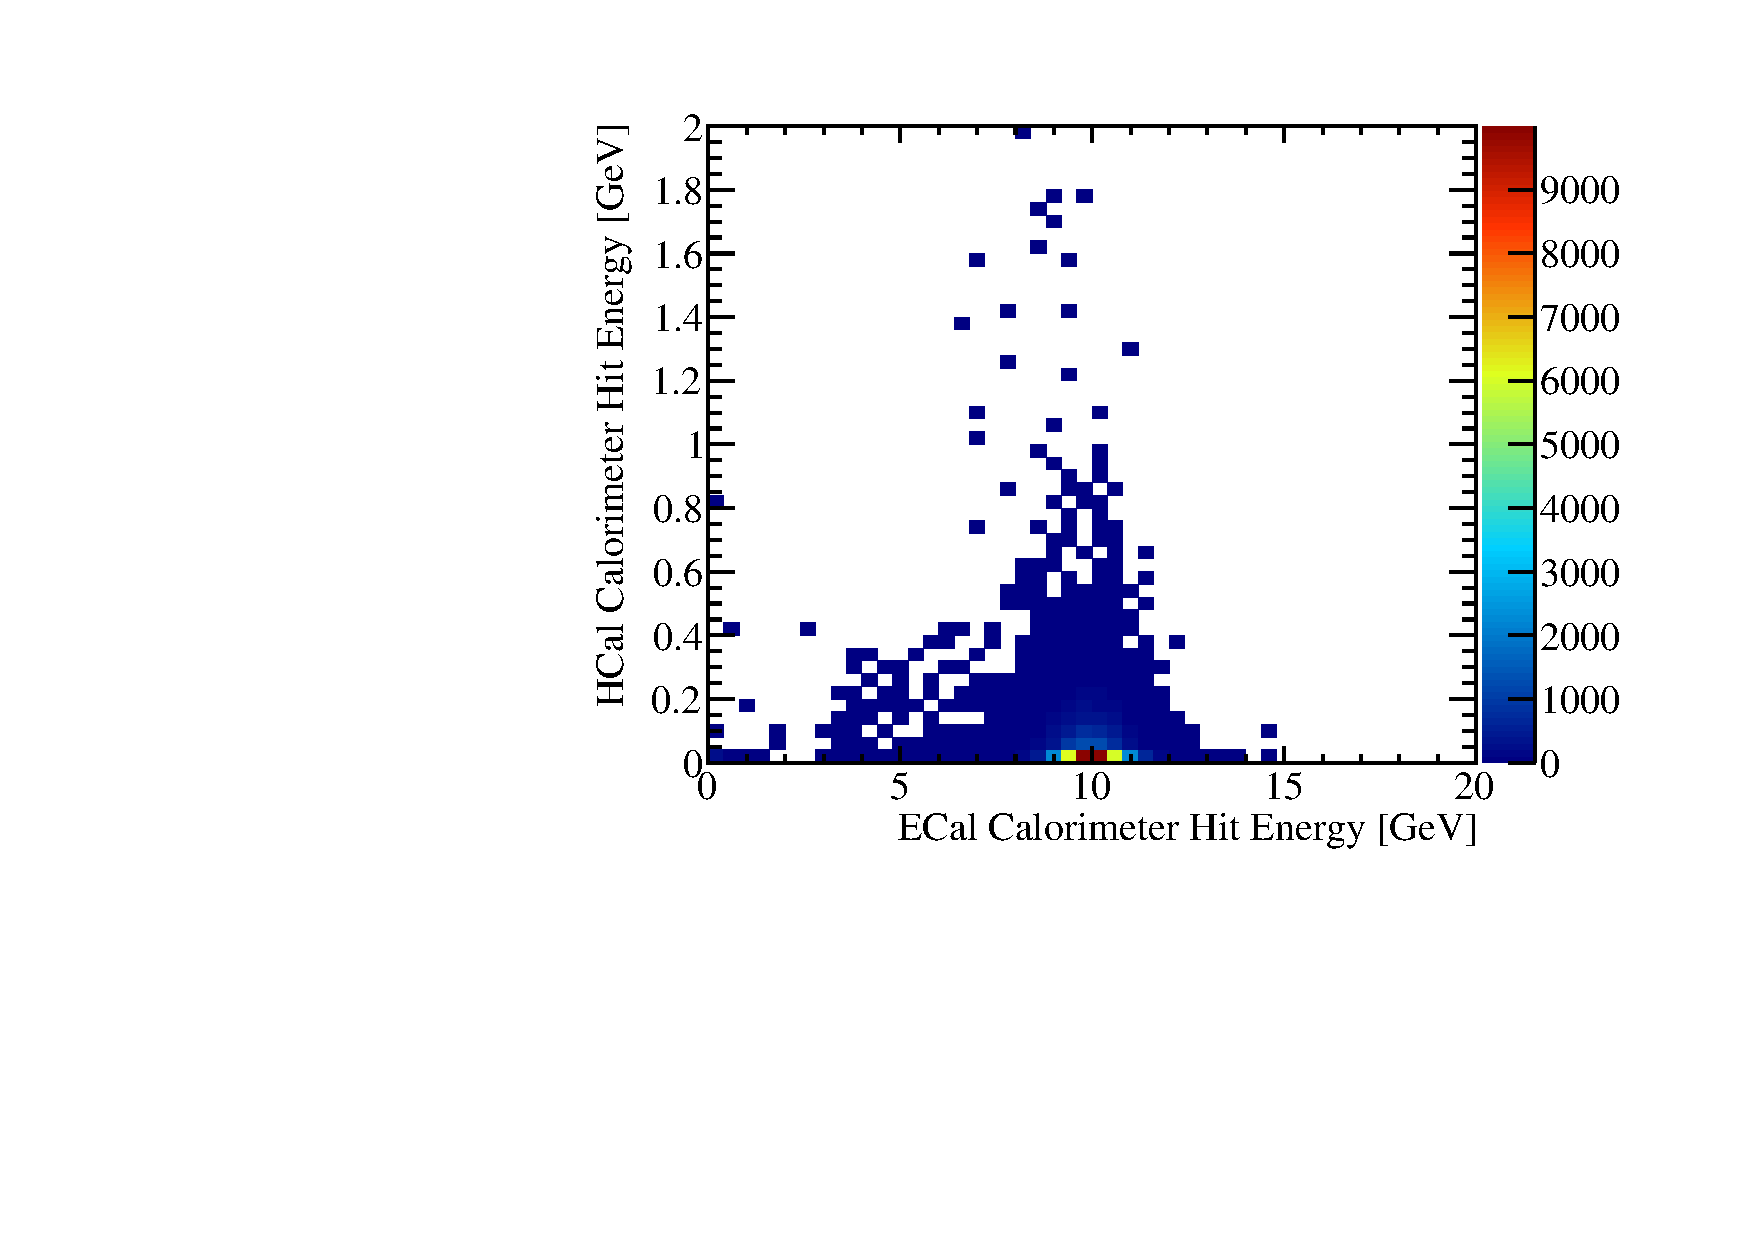
\includegraphics[width=0.5\textwidth]{EnergyEstimators/Plots/Calibration/Digitsation/ECal/ECalHCalPhotonSplit.pdf}}
\subfloat[]{\label{fig:ecaldigiselection}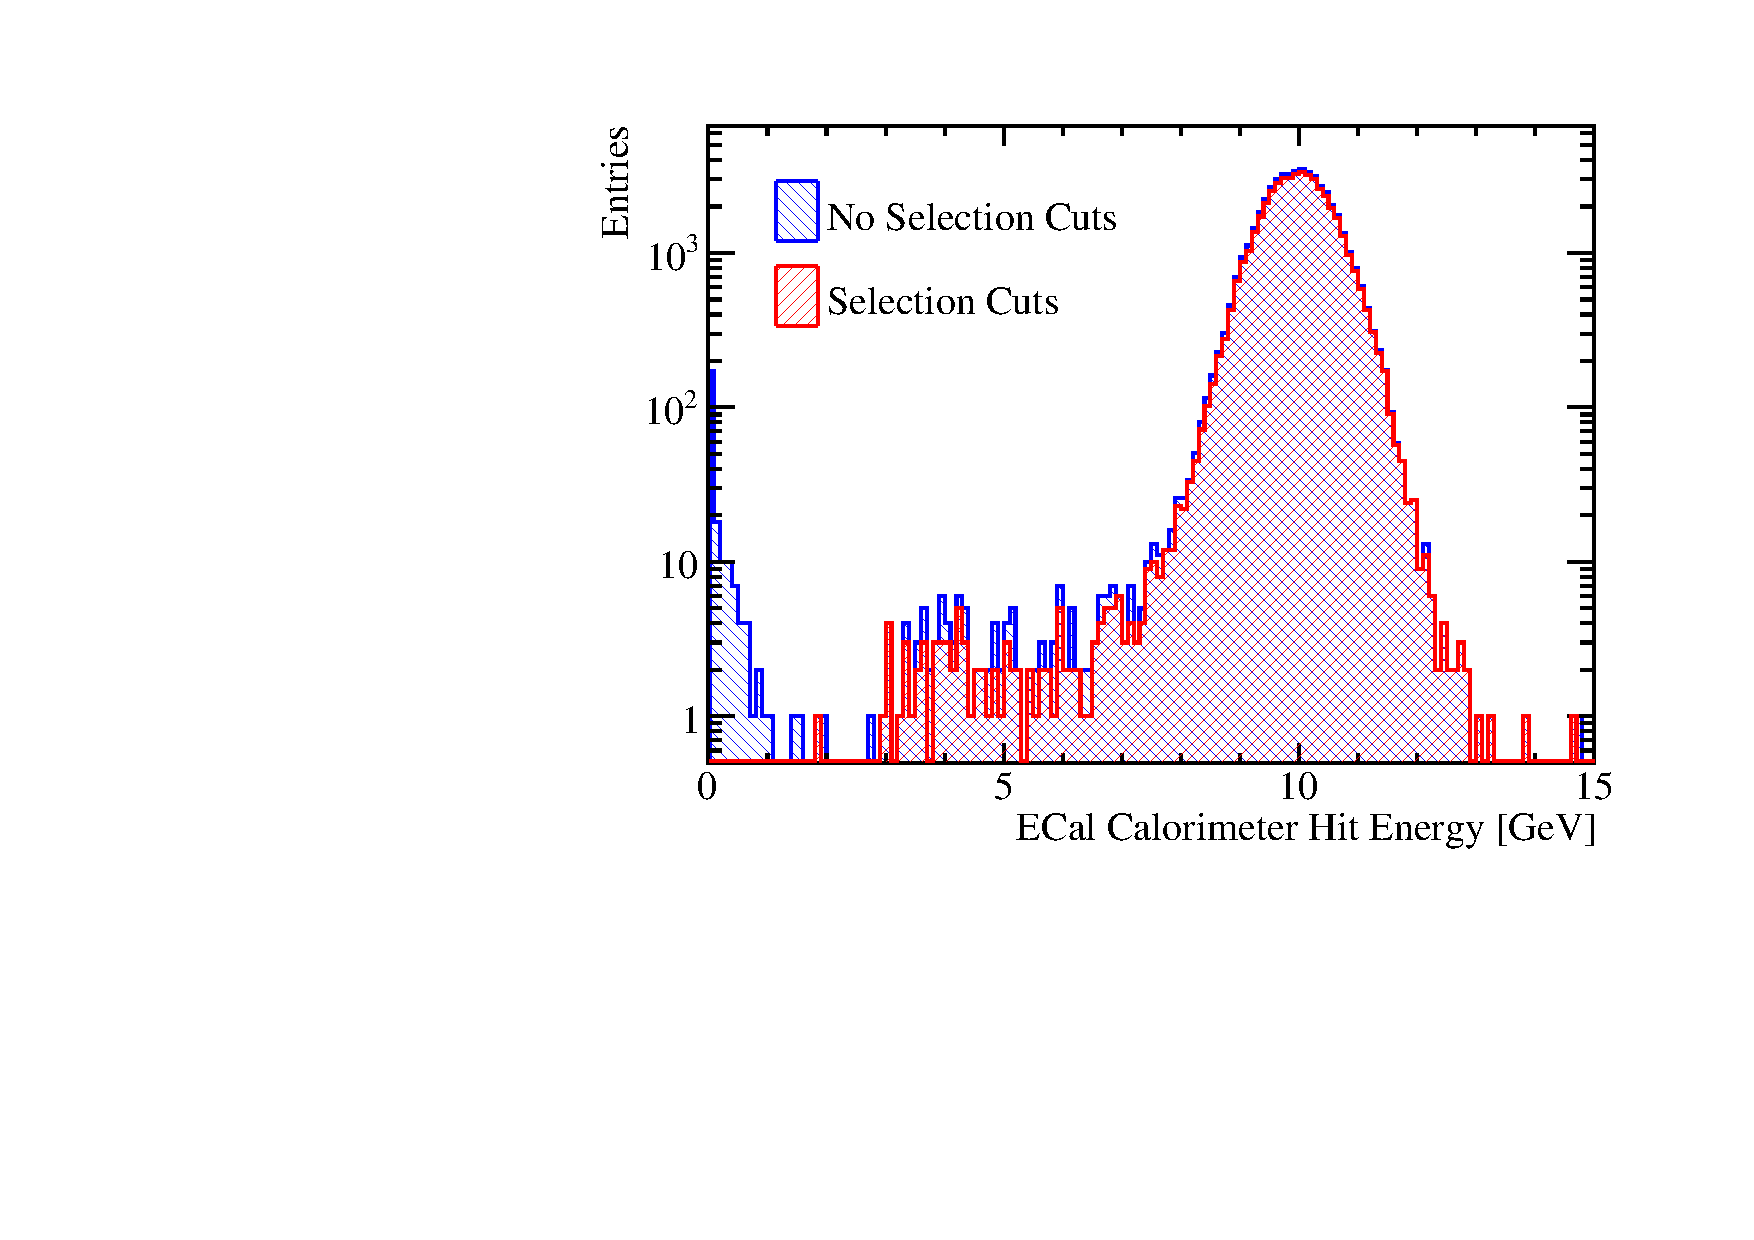
\includegraphics[width=0.5\textwidth]{EnergyEstimators/Plots/Calibration/Digitsation/ECal/DigitisationECalSelection.pdf}}
\caption[\protect\subref{fig:ecaldigiphotonsplit} The sum of calorimeter hit energies in ECal and HCal for 10 GeV $\gamma$ events.  \protect\subref{fig:ecaldigiselection} The sum of the ECal calorimeter hit energies for 10 GeV $\gamma$ events with and without the selection cuts.]{\protect\subref{fig:ecaldigiphotonsplit} The sum of calorimeter hit energies in ECal and HCal for 10 GeV $\gamma$ events.  \protect\subref{fig:ecaldigiselection} The sum of the ECal calorimeter hit energies for 10 GeV $\gamma$ events with and without the selection cuts.}
\label{fig:ecaldigi}
\end{figure}

The calibration of the digitisation in the ECal is an iterative procedure, which begins with the simulation of single $\gamma$ events using a trial calibration, with digitisation constant in the ECal $\alpha^{0}_{\text{ECal}}$.  Next the distribution of the sum of calorimeter hit energies within the ECal is produced for events passing the selection cuts, as shown in figure \ref{fig:ecaldigiselection}.  For an ideal calorimeter this distribution should be Gaussian, as was described in chapter \ref{chap:detopt}, therefore, a Gaussian fit is applied to this distribution and the mean, $E_{\text{Fit}}$, extracted.  To remove the effect of any outliers in this distribution, the fit is applied to the range of data with the smallest root mean square that contains at least 90 \% of the data.  An example of such a fit is shown in figure \ref{fig:ecaldigifit}.  In the case of ideal calibration the mean of this fit, $E_{\text{Fit}}$, would be equal $E_{MC}$.  It is assumed that any difference between the two is due to the calibration and to correct for this the digitisation constant from the trial calibration, $\alpha^{0}_{\text{ECal}}$, is rescaled by the ratio of the $E_{MC}$ to $E_{\text{Fit}}$:
%
\begin{equation}
\alpha^{0}_{\text{ECal}} \rightarrow \alpha_{\text{ECal}} = \alpha^{0}_{\text{ECal}} \times \frac{E_{MC}}{E_{Fit}}\text{ ,}
\end{equation}
%
This procedure is then repeated until the $E_{\text{Fit}}$ falls within a specified tolerance.  The tolerance applied here was $|E_{\text{Fit}} - E_{\text{MC}}| < E_{\text{MC}} \times 5 \%$.  The binning used for the fitted histogram is chosen such that the bin width is equal to the desired tolerance on $E_{\text{Fit}}$ e.g. $E_{\text{MC}} \times 5 \% = 0.5$ GeV.  This tolerance is somewhat loose, however, it is tight enough to ensure successful application of PFA.  It should also be emphasised that the PFO energies used for downstream analyses have the electromagnetic and hadronic energy scale corrections applied, which are calibrated to a much tighter accuracy.

\begin{figure}[h!]
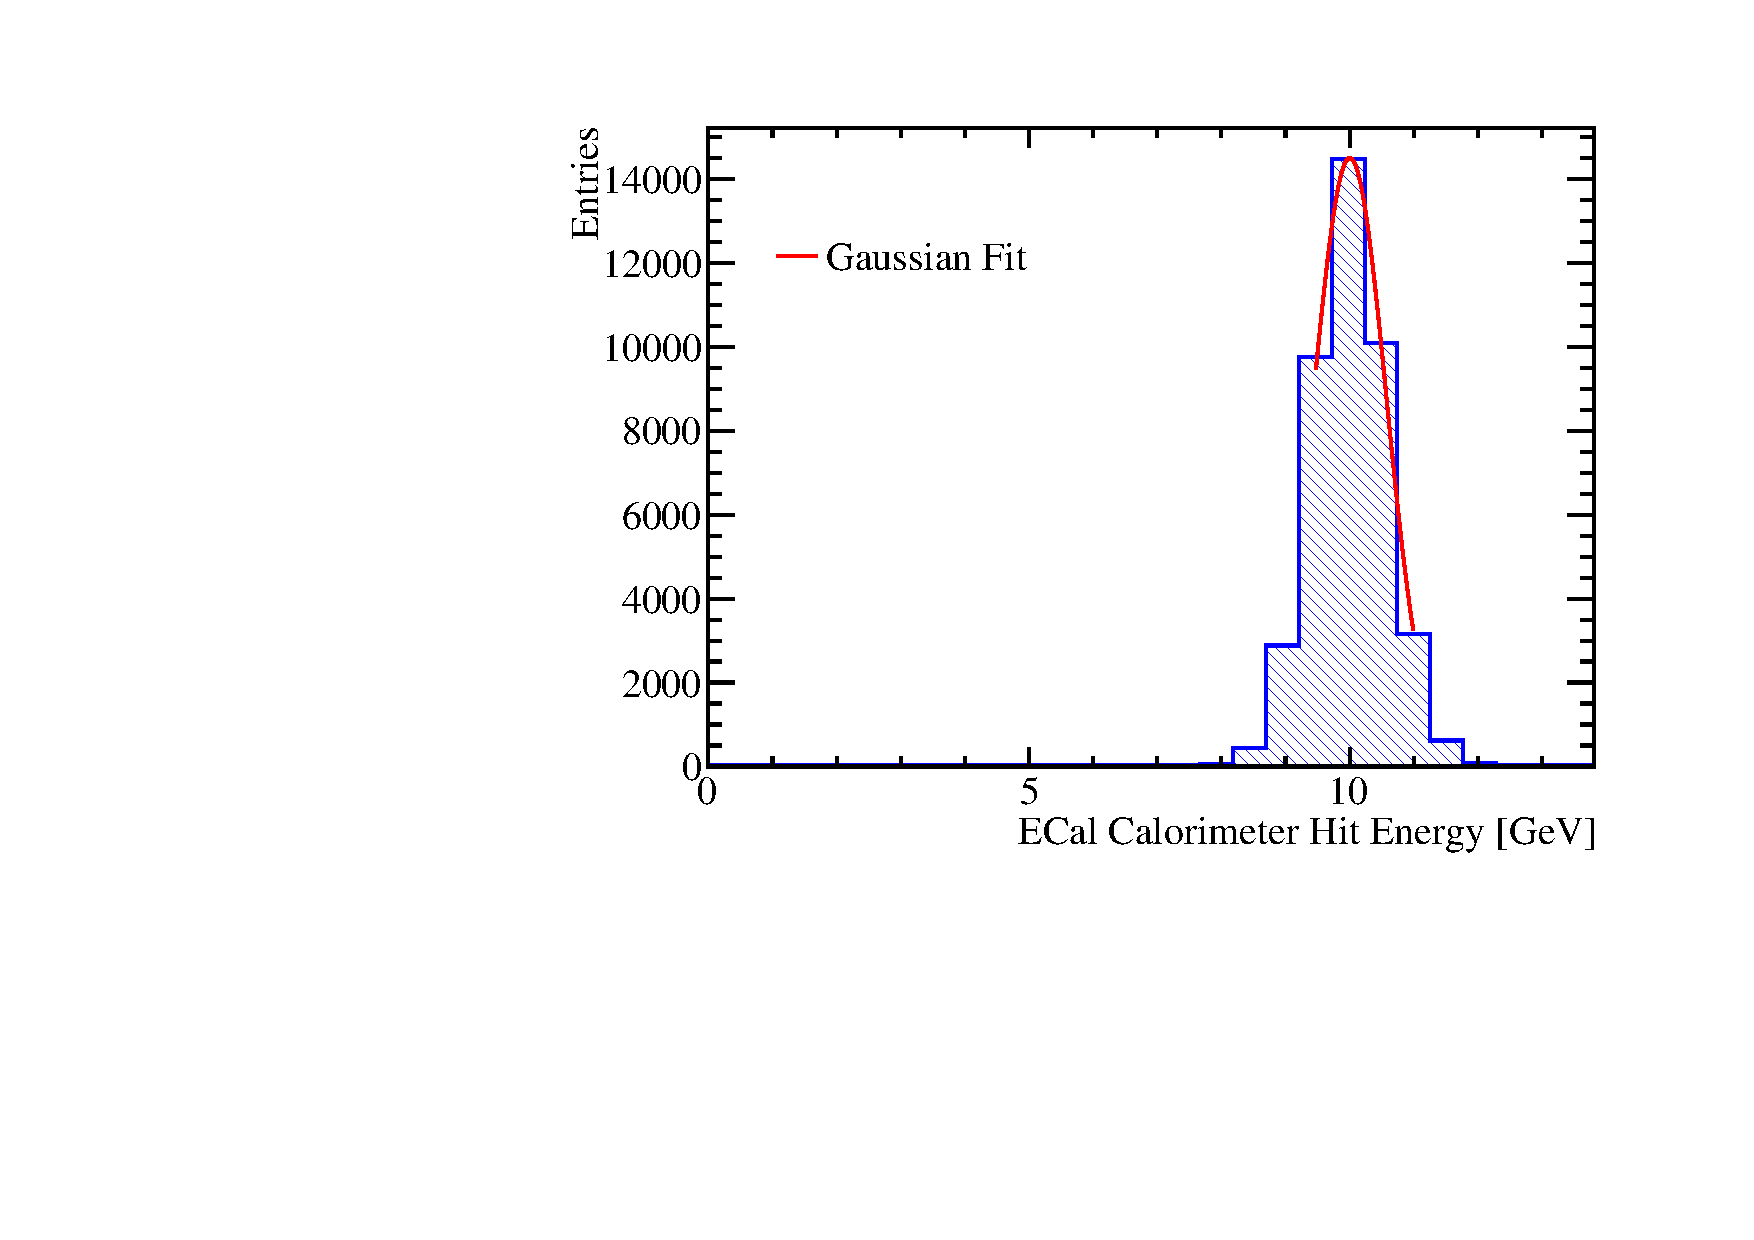
\includegraphics[width=0.5\textwidth]{EnergyEstimators/Plots/Calibration/Digitsation/ECal/DigitisationECalFit.pdf}
\caption[Gaussian fit to sum of the ECal calorimeter hit energies for 10 GeV $\gamma$ events with selection cuts.  The coarse binning reflects the tolerance on the digitisation constant calibration.]{Gaussian fit to sum of the ECal calorimeter hit energies for 10 GeV $\gamma$ events with selection cuts.  The coarse binning reflects the tolerance on the digitisation constant calibration.}
\label{fig:ecaldigifit}
\end{figure}

%========================================================================================

\subsubsection{HCal Digitisation Implementation}
\label{sec:hcaldigi}
The calibration for the digitisation in the HCal proceeds in a similar manor to that described for the ECal with a few key differences.  This calibration uses $K^{0}_{L}$ events at $E_{MC} = 20$ GeV as these neutral hadrons will deposit the bulk of their energy in the HCal.  The higher energy, with respect to the ECal digitisation, is used to create larger particle showers that sample deeper into the HCal.  As the $K^{0}_{L}$s must pass through the ECal before arriving at the HCal and, as the ECal contains $\approx 1 \lambda_{I}$, some of the $K^{0}_{L}$s begin showering in the ECal, as shown by figure \ref{fig:hcaldigikaonsplit}.  Such events are unsuitable for calibration of the HCal digitisation constants as rescaling $\alpha^{0}_{\text{HCal}}$ would not lead to a linear rescaling in $E_{\text{Fit}}$.  These events are vetoed in the even selection by requiring events deposit less than less than 5\% of $E_{MC}$ outside of the HCal.  In addition to this, the last layer of the HCal where energy is deposited is required to be in the innermost 90\% of the HCal.  This cut vetoes events that shower late in the HCal and deposit a significant amount of energy in the uninstrumented coil region of the detector.  The impact of these cuts on the sum of HCal calorimeter hit energies for the $E_{MC} = 20$ GeV $K^{0}_{L}$ events is shown in figure \ref{fig:hcaldigiselection}.  There are two HCal digitisation constants used in the detector simulation, one applied for the barrel and another for the endcap.  This is to account for differences in hadronic shower dynamics between the two, such as differing magnetic field configurations in the barrel and endcap.  Both parameters are calibrated in the same manor, but have different cuts on $\theta$, the polar angle of the $K^{0}_{L}$.  For the barrel region of the HCal events are selected if $0.2 < \text{cos}(\theta) < 0.6$, while for the endcap events are selected if $0.8 < \text{cos}(\theta) < 0.9$.  These angular cuts are conservative to account for the transverse profile of the hadronic showers and ensure that they are confined to the relevant sub-detector.  One further difference to the ECal digitisation procedure is that the target reconstructed energy for the $K^{0}_{L}$ samples is the kinetic energy as opposed to the total energy.  As the majority of the neutral hadrons appearing in jets are neutrons and their accessible energy is their kinetic energy, calibrating to the kinetic energy should give the best performance for jet reconstruction.  

\begin{figure}[h!]
\subfloat[]{\label{fig:hcaldigikaonsplit}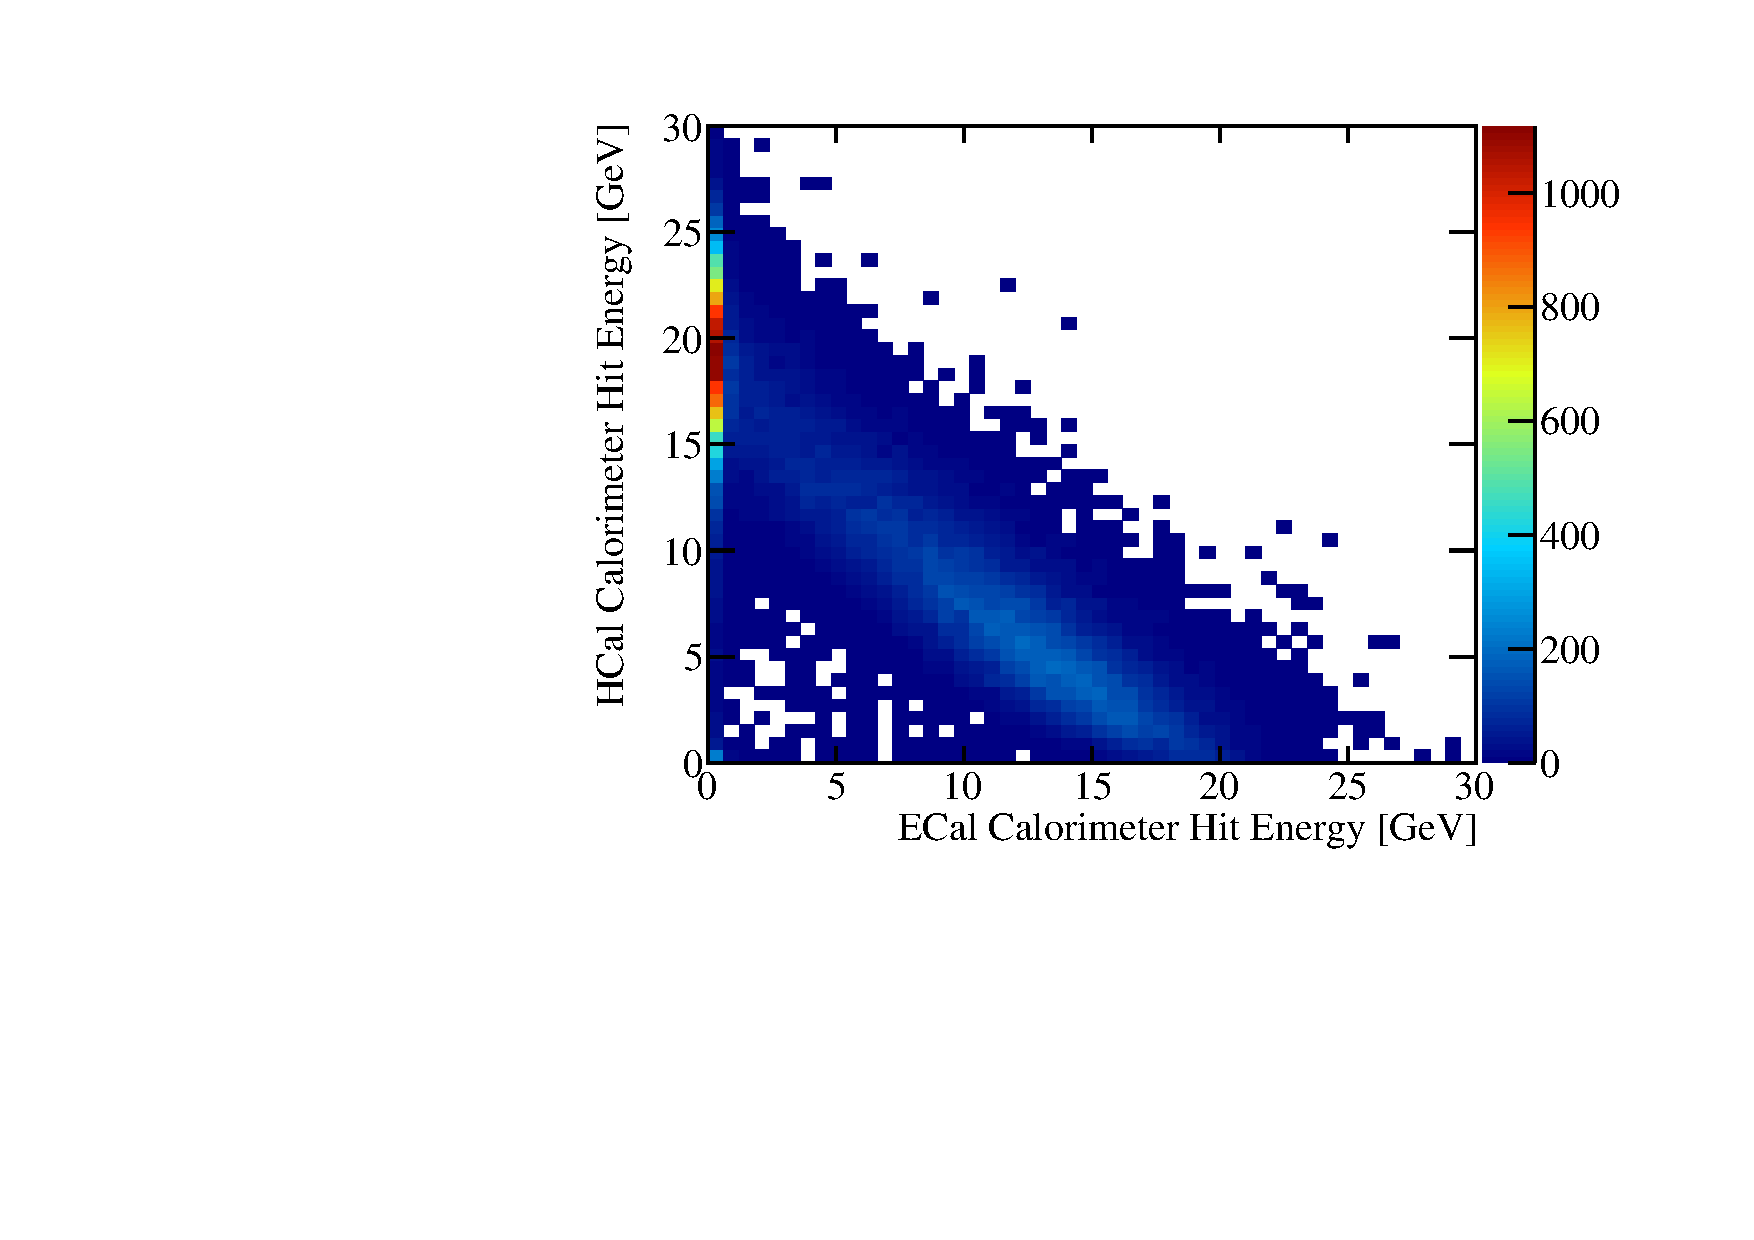
\includegraphics[width=0.5\textwidth]{EnergyEstimators/Plots/Calibration/Digitsation/HCal/ECalHCalKaon0LSplit.pdf}}
\subfloat[]{\label{fig:hcaldigiselection}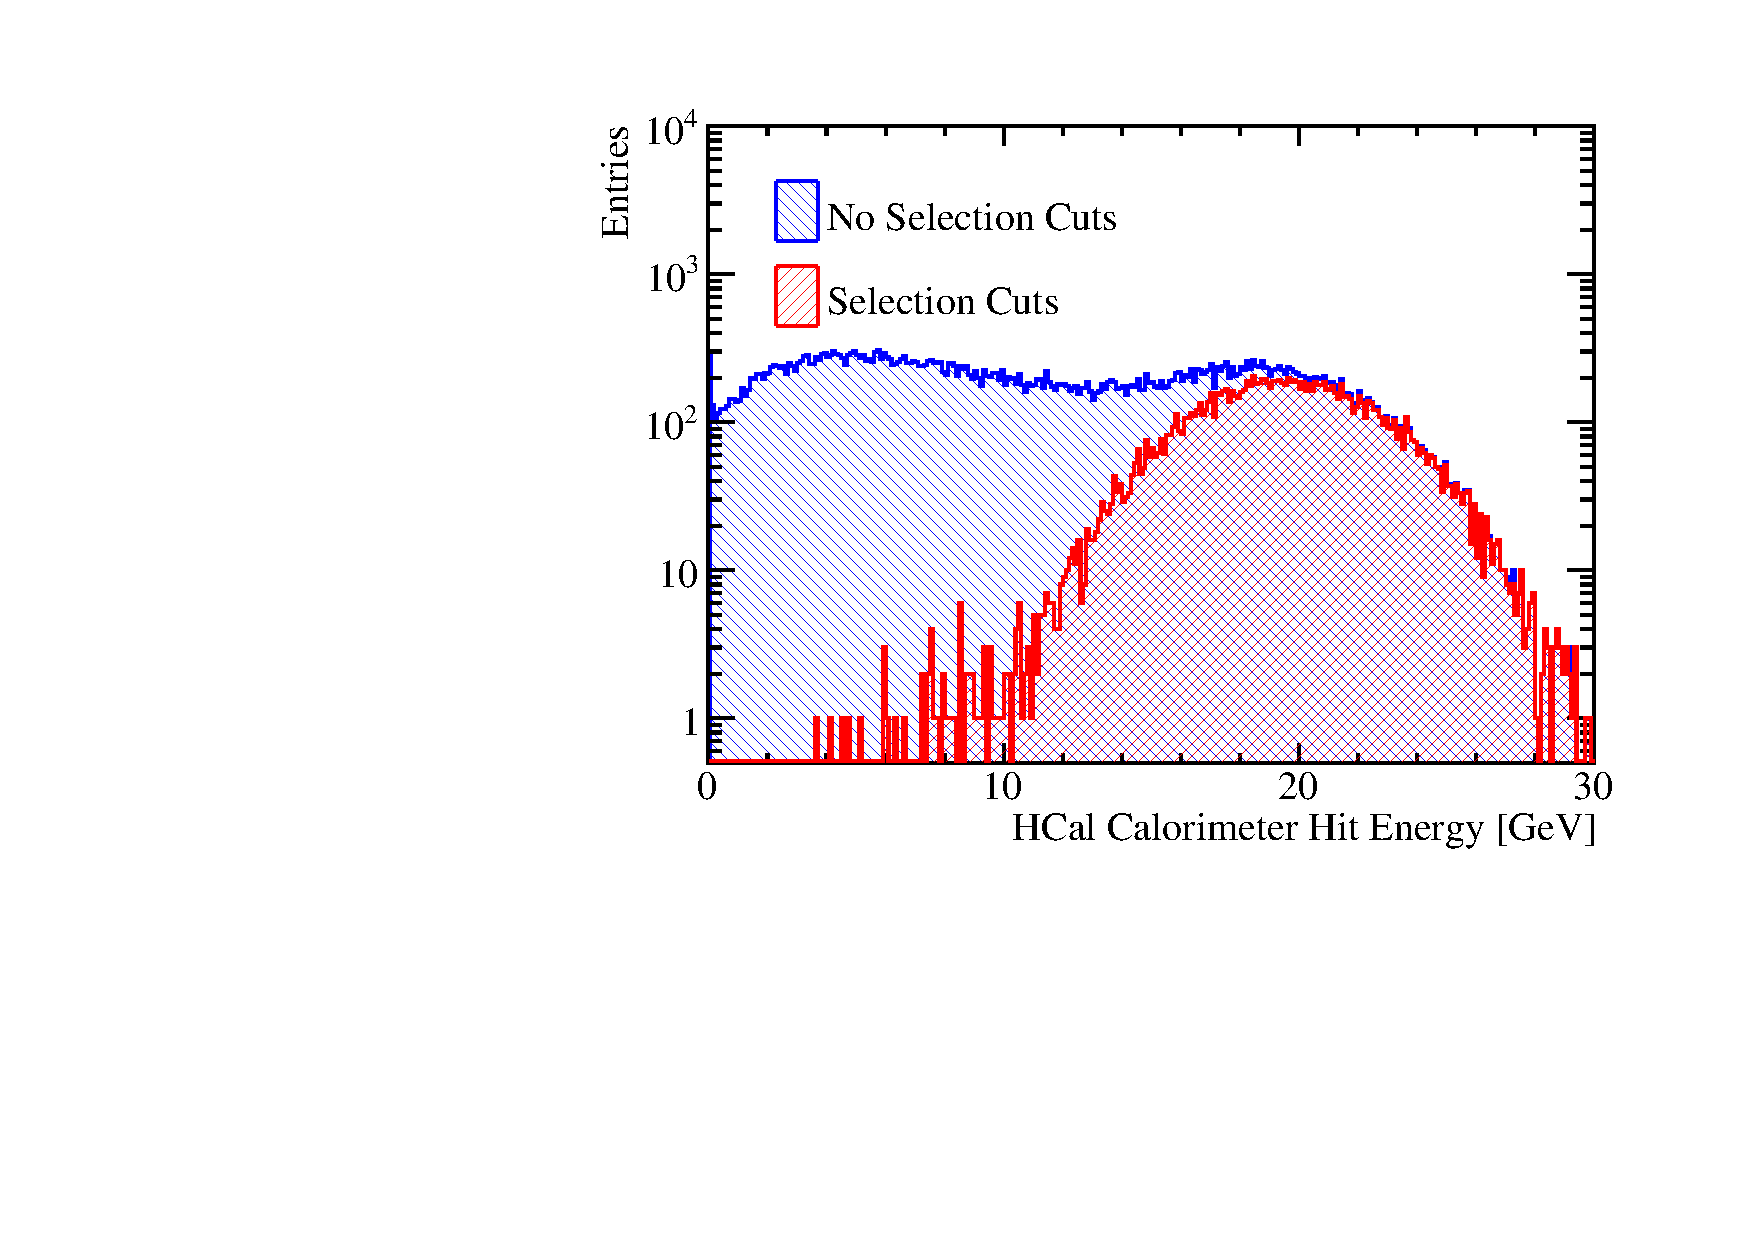
\includegraphics[width=0.5\textwidth]{EnergyEstimators/Plots/Calibration/Digitsation/HCal/DigitisationHCalSelection.pdf}}
\caption[\protect\subref{fig:hcaldigikaonsplit} Sum of calorimeter hit energies in ECal and HCal for 20 GeV $K^{0}_{L}$ events.  \protect\subref{fig:hcaldigiselection} Sum of the HCal calorimeter hit energies for a 20 GeV $K^{0}_{L}$ events with and without the selection cuts.]{\protect\subref{fig:hcaldigikaonsplit} Sum of calorimeter hit energies in ECal and HCal for 20 GeV $K^{0}_{L}$ events.  \protect\subref{fig:hcaldigiselection} Sum of the HCal calorimeter hit energies for a 20 GeV $K^{0}_{L}$ events with and without the selection cuts.}
\label{fig:hcaldigi}
\end{figure}

Using these cuts the calibration procedure for the digitisation of the HCal barrel and endcap proceeds in the same manor as was described for the ECal, the details of which can be found in section \ref{sec:ecaldigi}.  Examples of the Gaussian fits applied to the sum of the calorimeter hit energies in the HCal barrel and endcap can be found in figure \ref{fig:hcaldigifit}.  

\begin{figure}[h!]
\subfloat[HCal barrel.]{\label{fig:hcaldigibarrel}\includegraphics[width=0.5\textwidth]{EnergyEstimators/Plots/Calibration/Digitsation/HCal/DigitisationHCalbarrelFit.pdf}}
\subfloat[HCal endcap.]{\label{fig:hcaldigiendcap}\includegraphics[width=0.5\textwidth]{EnergyEstimators/Plots/Calibration/Digitsation/HCal/DigitisationHCalendcapFit.pdf}}
\caption[Gaussian fit to sum of the HCal calorimeter hit energies for 20 GeV $K^{0}_{L}$ events with selection cuts.]{Gaussian fit to sum of the HCal calorimeter hit energies for 20 GeV $K^{0}_{L}$ events with selection cuts.}
\label{fig:hcaldigifit}
\end{figure}

%========================================================================================

\subsubsection{HCal Ring Digitisation Implementation}
\label{sec:hcalringdigi}
The HCal ring, illustrated in figure \ref{fig:calorimeters}, also has an independent digitisation constant to account for any difference in the hadronic shower development between the ring, barrel and endcap.  The procedure used to calibrate this constant has to differs from that presented in section \ref{sec:hcaldigi} as it is unfeasible, due to the depth of the ring, to produce events that are wholly contained within it.  Fortunately, the size of the HCal ring means it plays a minimal role in the reconstruction, so precise calibration is not crucial.  To ensure that the calibration is approximately correct for the HCal ring, $\alpha_{\text{HCal ring}}$ is assumed to equal $\alpha_{\text{HCal endcap}}$ multiplied by several factors designed to accounts for changes in the active layer thickness, absorber layer thickness and the MIP response between the HCal endcap and ring.  In detail:
%
\begin{equation}
\alpha_{\text{HCal ring}} = \alpha_{\text{HCal endcap}} \times \frac{\langle \text{cos}(\theta_\text{endcap}) \rangle}{\langle \text{cos}(\theta_\text{ring}) \rangle} \times \frac{P_\text{endcap} }{P_\text{ring} } \times \frac{L^{Absorber}_\text{endcap}}{L^{Absorber}_\text{ring} } \times \frac{L^{Active}_\text{ring}}{L^{Active}_\text{endcap}} \text{ ,}
\end{equation}
%
\noindent where $\theta$ is the incident angle of the incoming particle to the calorimeter determined using the 20 GeV $K^{0}_{L}$ events, $L^{Active}$ is the active layer thickness and $L^{Absorber}$ is the absorber layer thickness. $P$ is the position of the MIP peak in the distribution of active layer hit energies, which has been corrected so that the MIP appears to enter the calorimeter at normal incidence, and is determined using 10 GeV $\mu^{-}$ events.  Details on how $P$ is determined can be found in section \ref{sec:mipresponse}.

\begin{figure}[h!]
\subfloat[]{\label{fig:ecal}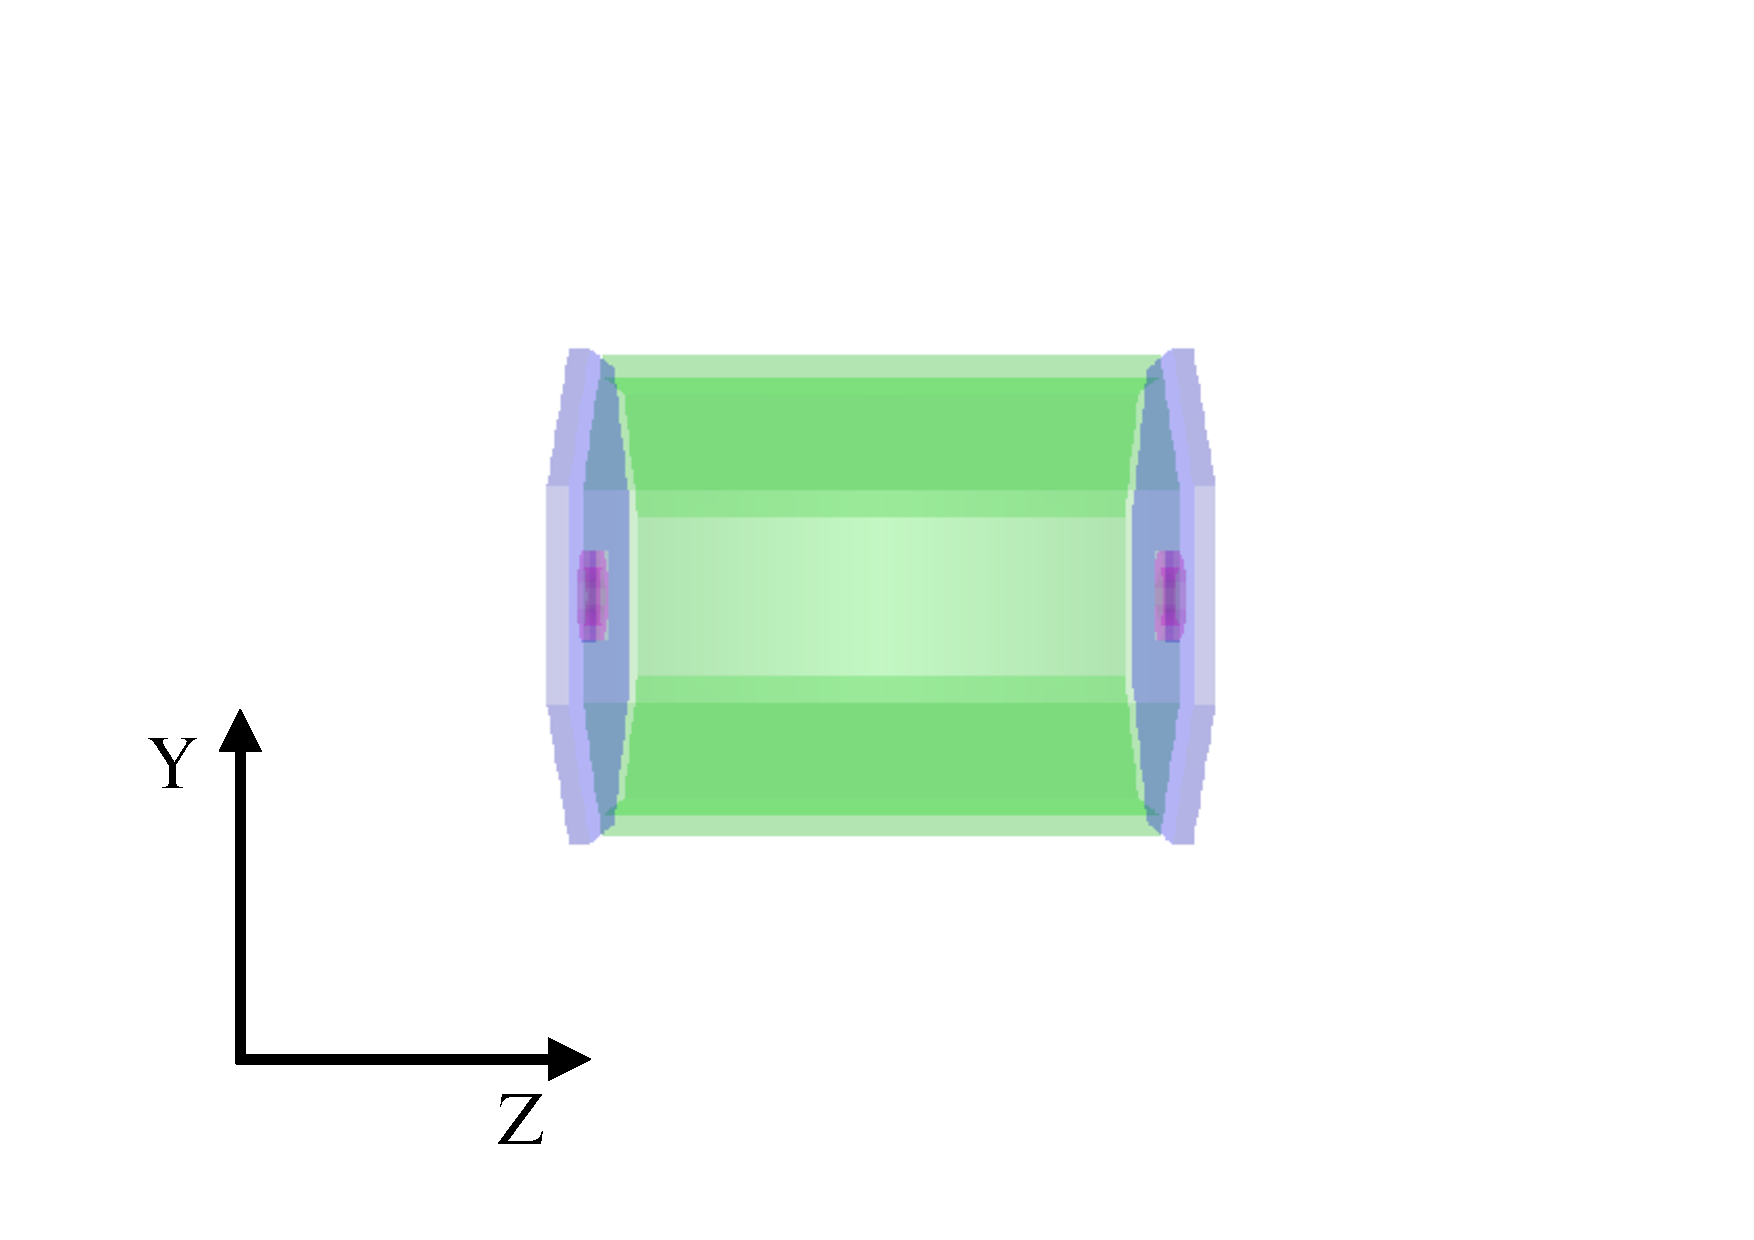
\includegraphics[width=0.33\textwidth]{EnergyEstimators/Plots/Calibration/VisualDisplay/ECalWithScale.pdf}}
\subfloat[]{\label{fig:hcal}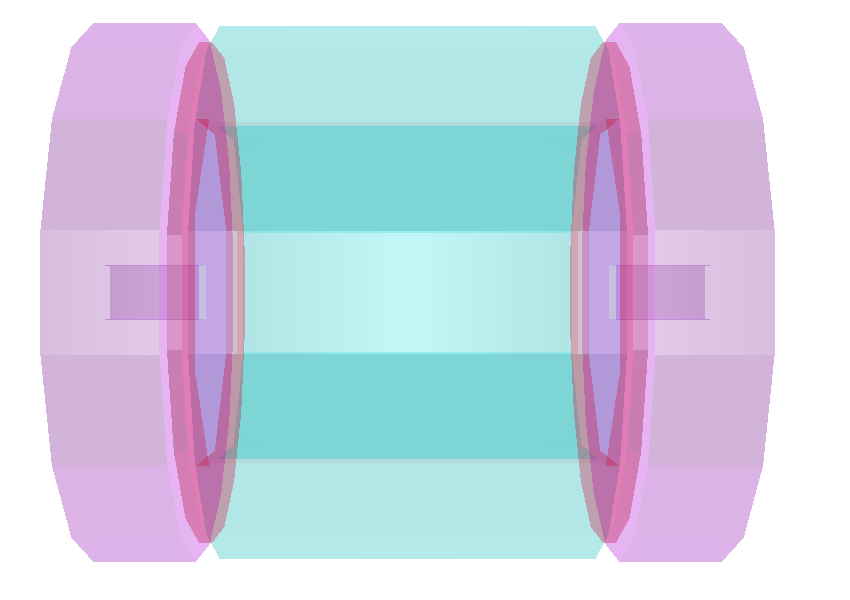
\includegraphics[width=0.33\textwidth]{EnergyEstimators/Plots/Calibration/VisualDisplay/HCal.png}}
\subfloat[]{\label{fig:hcalring}\includegraphics[width=0.33\textwidth]{EnergyEstimators/Plots/Calibration/VisualDisplay/HCalring.png}}
\caption[A PandoraPFA event display showing the nominal ILD calorimeters.  \protect\subref{fig:ecal} the ECal, \protect\subref{fig:hcal} the full HCal and \protect\subref{fig:hcalring} the HCal ring.]{A PandoraPFA event display showing the nominal ILD calorimeters.  \protect\subref{fig:ecal} the ECal, \protect\subref{fig:hcal} the full HCal and \protect\subref{fig:hcalring} the HCal ring.}
\label{fig:calorimeters}
\end{figure}

%========================================================================================

\subsection{MIP Scale Determination}
\label{sec:mipresponse}
The digitiser MIP scale was defined as the, non-zero, peak in the distribution of the active layer calorimeter hit energies for normally incident 10~GeV $\mu^{-}$ \cite{Bichsel:2004ej}, as shown in figure \ref{fig:digitisermip}.  This distribution is made for each calorimeter where the MIP scale needs to be determined.  As the average energy deposited per hit in a given sub-detector is relevant for setting the MIP scale, as opposed to the total energy deposited in a sub-detector, no selection cuts are required.  The sample of $\mu^{-}$ events used for setting the MIP scale were generated isotropically.  When populating the active layer energy distribution a direction correction factor of $\text{cos}(\theta)$, where $\theta$ is the incident angle of the $\mu^{-}$ to the calorimeter hit, was applied to the hit energy to generate the effect of having the $\mu^{-}$ enter the calorimeter at normal incidence.  The MIP scale was determined separately for the ECal, HCal barrel, HCal endcap and HCal ring, however, only a single HCal MIP scale, taken as the HCal barrel, was required by the digitisation processor.  The HCal endcap and ring MIP scales were calculated for the purposes of the HCal ring digitisation described in section \ref{sec:hcalringdigi}.  No MIP scale setting was required in the digitisation processor for the muon chamber.  

\begin{figure}[h!]
\subfloat[]{\label{fig:digitisermipecal}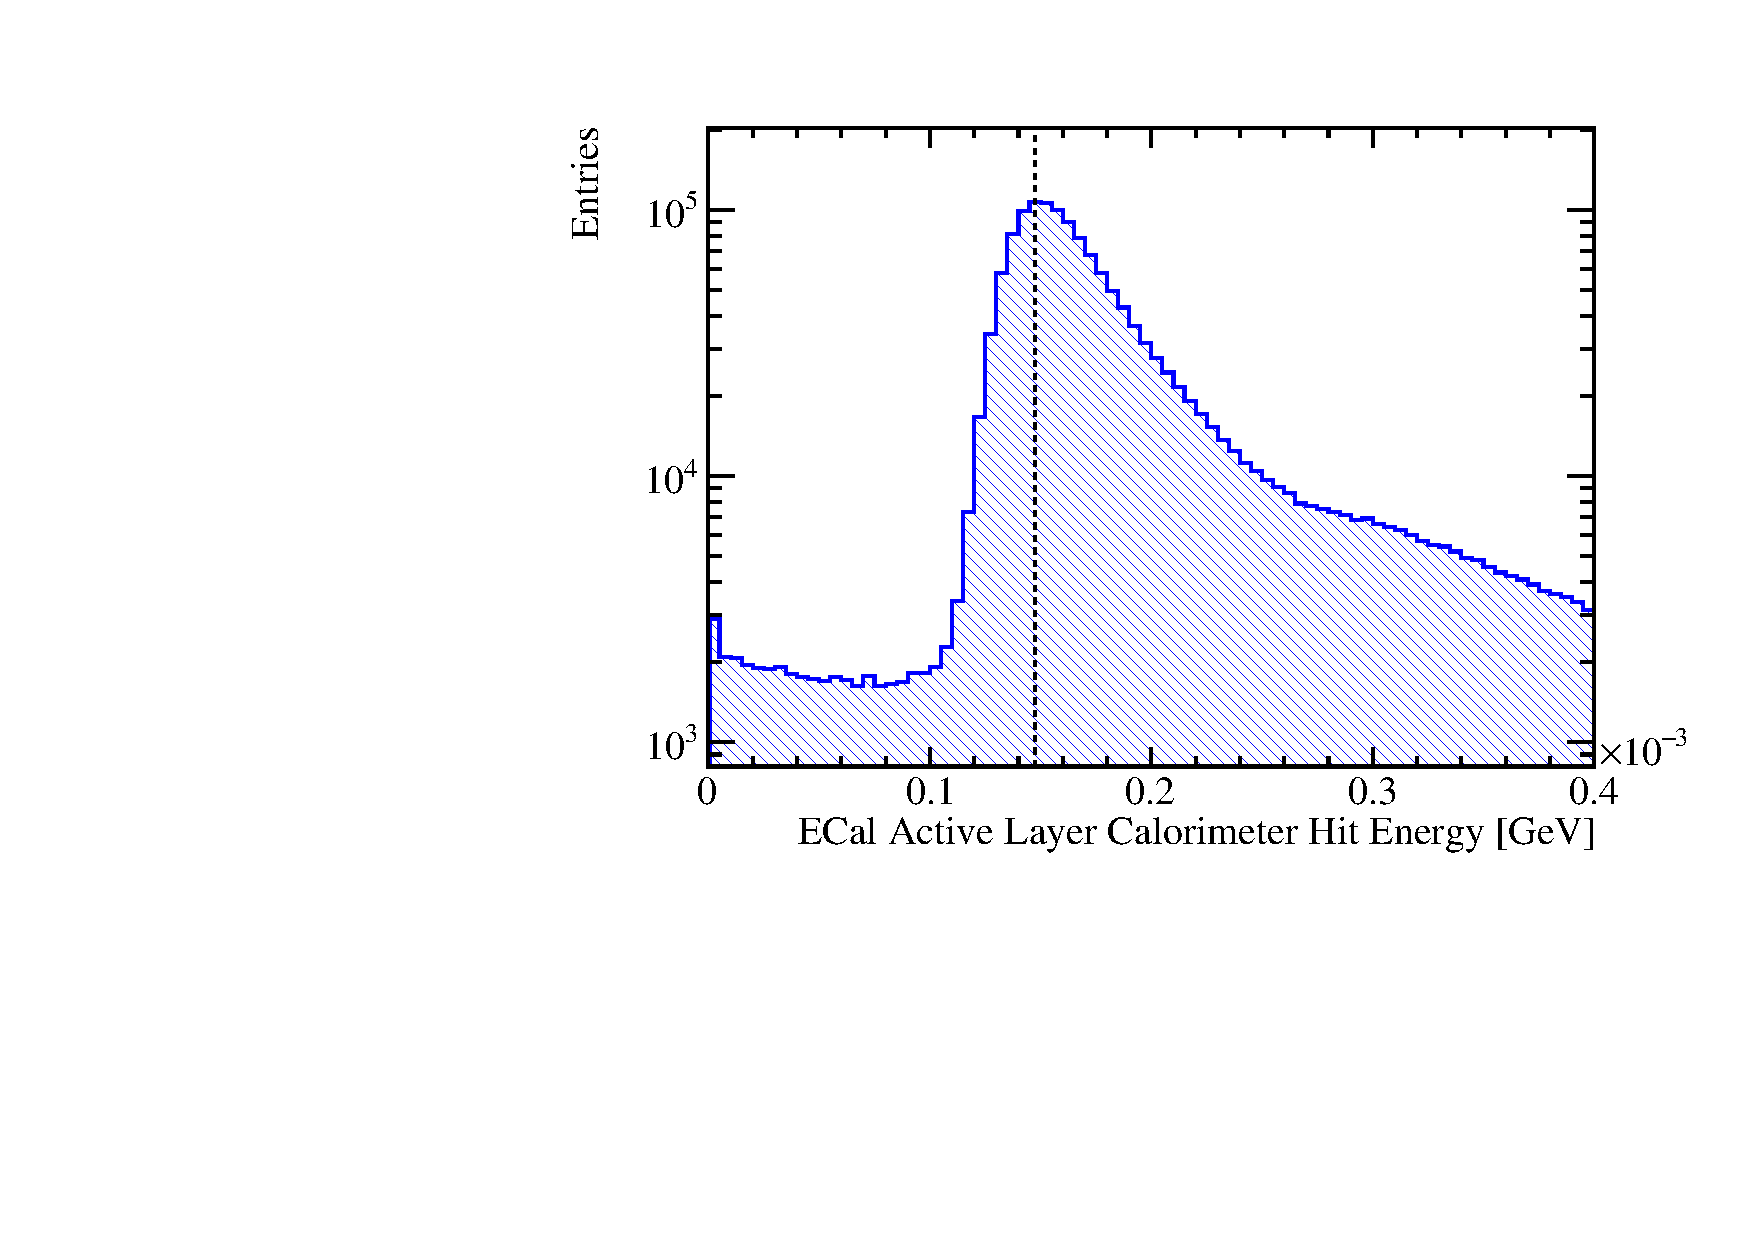
\includegraphics[width=0.5\textwidth]{EnergyEstimators/Plots/Calibration/MIPScale/Digitiser/MIPScaleDigitiserECal.pdf}}
\subfloat[]{\label{fig:digitisermiphcalbarrel}\includegraphics[width=0.5\textwidth]{EnergyEstimators/Plots/Calibration/MIPScale/Digitiser/MIPScaleDigitiserHCalbarrel.pdf}} \\
\subfloat[]{\label{fig:digitisermiphcalendcap}\includegraphics[width=0.5\textwidth]{EnergyEstimators/Plots/Calibration/MIPScale/Digitiser/MIPScaleDigitiserHCalendcap.pdf}}
\subfloat[]{\label{fig:digitisermiphcalring}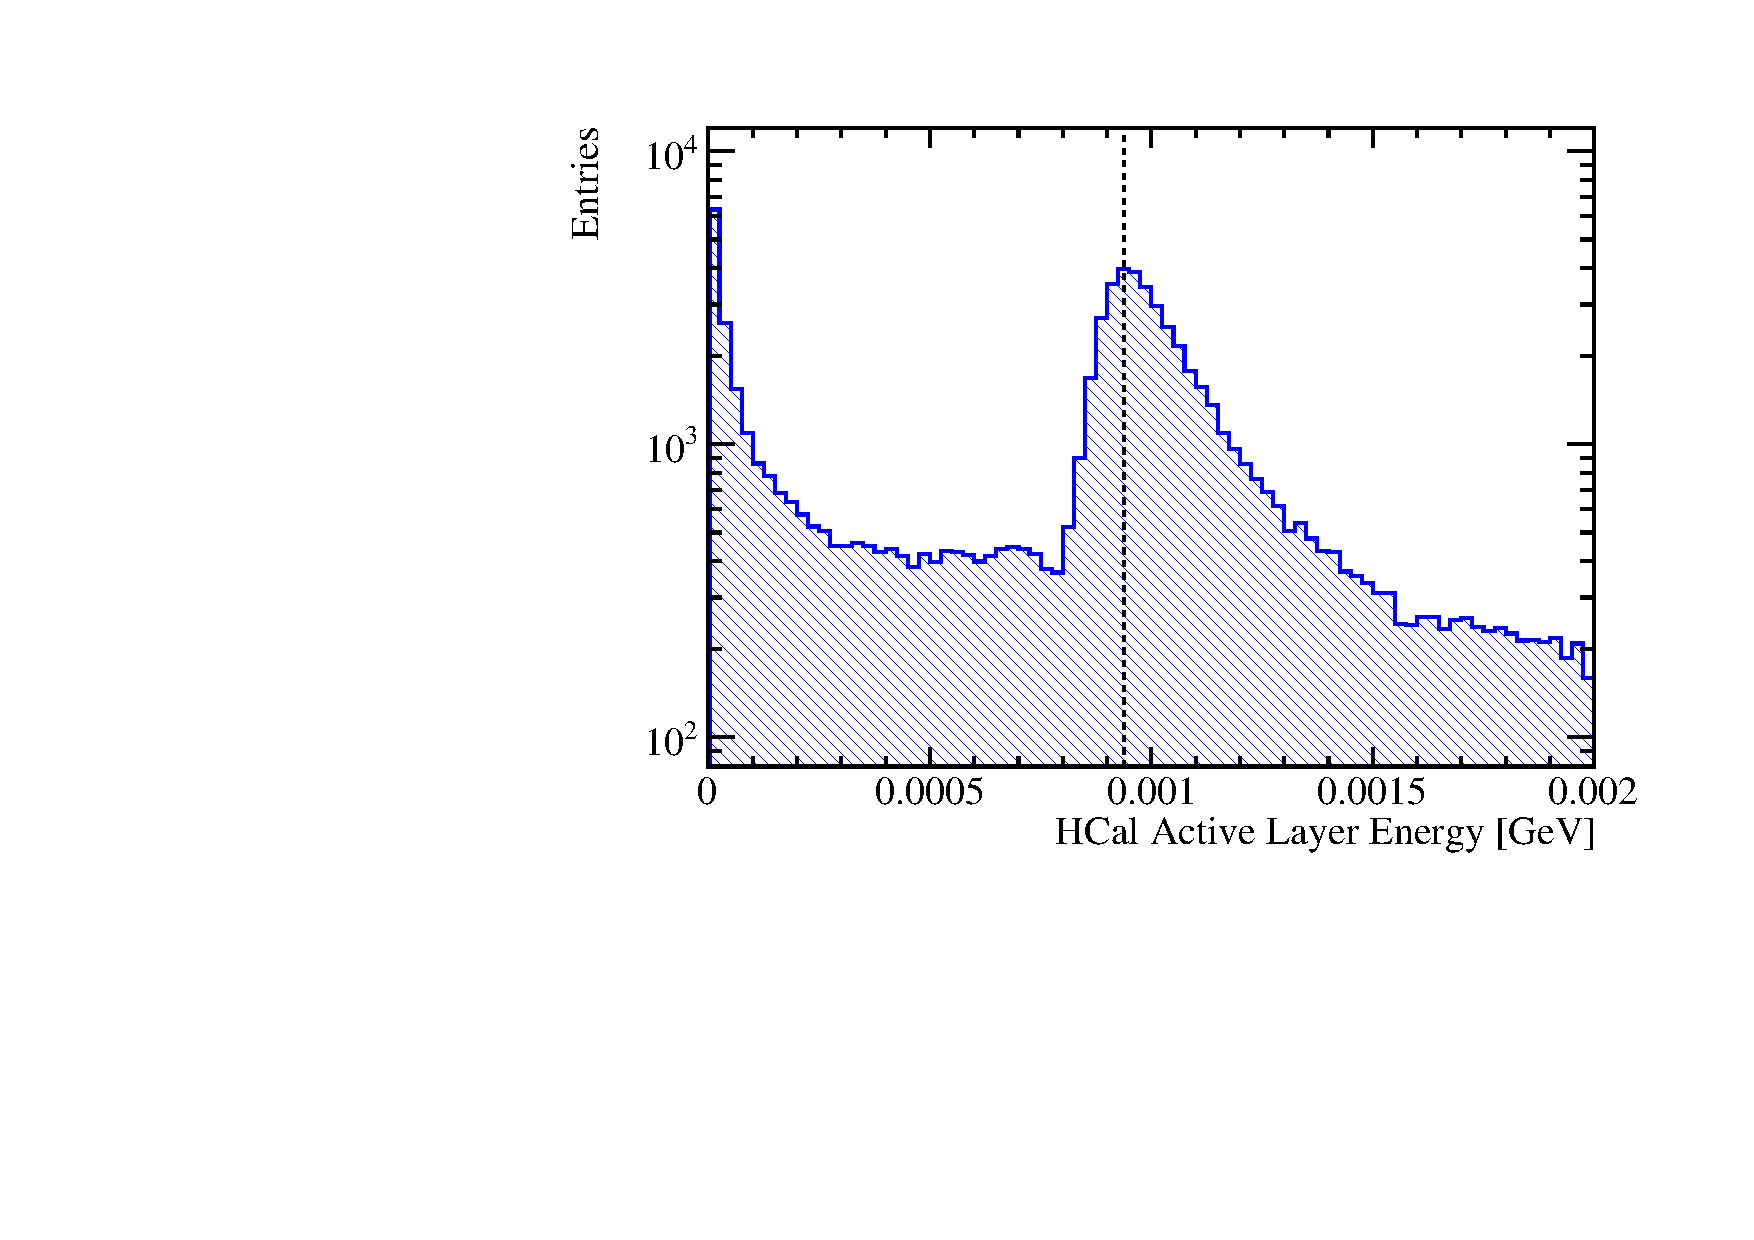
\includegraphics[width=0.5\textwidth]{EnergyEstimators/Plots/Calibration/MIPScale/Digitiser/MIPScaleDigitiserHCalOther.pdf}}
\caption[The active layer calorimeter hit energy distributions for \protect\subref{fig:digitisermipecal} the ECal, \protect\subref{fig:digitisermiphcalbarrel} the HCal barrel, \protect\subref{fig:digitisermiphcalendcap} the HCal endcap and \protect\subref{fig:digitisermiphcalring} the HCal ring for 10 GeV $\mu^{-}$ events.]{The active layer calorimeter hit energy distributions for \protect\subref{fig:digitisermipecal} the ECal, \protect\subref{fig:digitisermiphcalbarrel} the HCal barrel, \protect\subref{fig:digitisermiphcalendcap} the HCal endcap and \protect\subref{fig:digitisermiphcalring} the HCal ring for 10 GeV $\mu^{-}$ events.}
\label{fig:digitisermip}
\end{figure}

A similar procedure was employed for calculation of the MIP peak in PandoraPFA.  One important difference was the distribution used for setting the MIP scale in PandoraPFA is the distribution of calorimeter hit energies, i.e. the energy in the active and absorber layers of a hit, and not just the active layer energies.  Examples of the distributions used to set the MIP scale in PandoraPFA can be found in figure \ref{fig:pandoramip}.  There are few populated low calorimeter hit energy bins in this these distributions due to cuts applied in the digitiser on the active layer energy.  The double peak structure observed in the ECal calorimeter hit energy distribution is due to the ECal absorber material thickness doubling in the back 10 layers of the ECal.  Further differences between the MIP scale setting in the digitiser and PandoraPFA are as follows: The MIP scale setting in PandoraPFA combines the HCal sub-detectors, the barrel, endcap and ring, together when creating the calorimeter hit energy distributions; PandoraPFA requires the MIP scale to be set in the muon chamber unlike the digitisation processor and, therefore, the muon chamber hit energy distribution must also be created.  

\begin{figure}
\subfloat[]{\label{fig:pandoramipecal}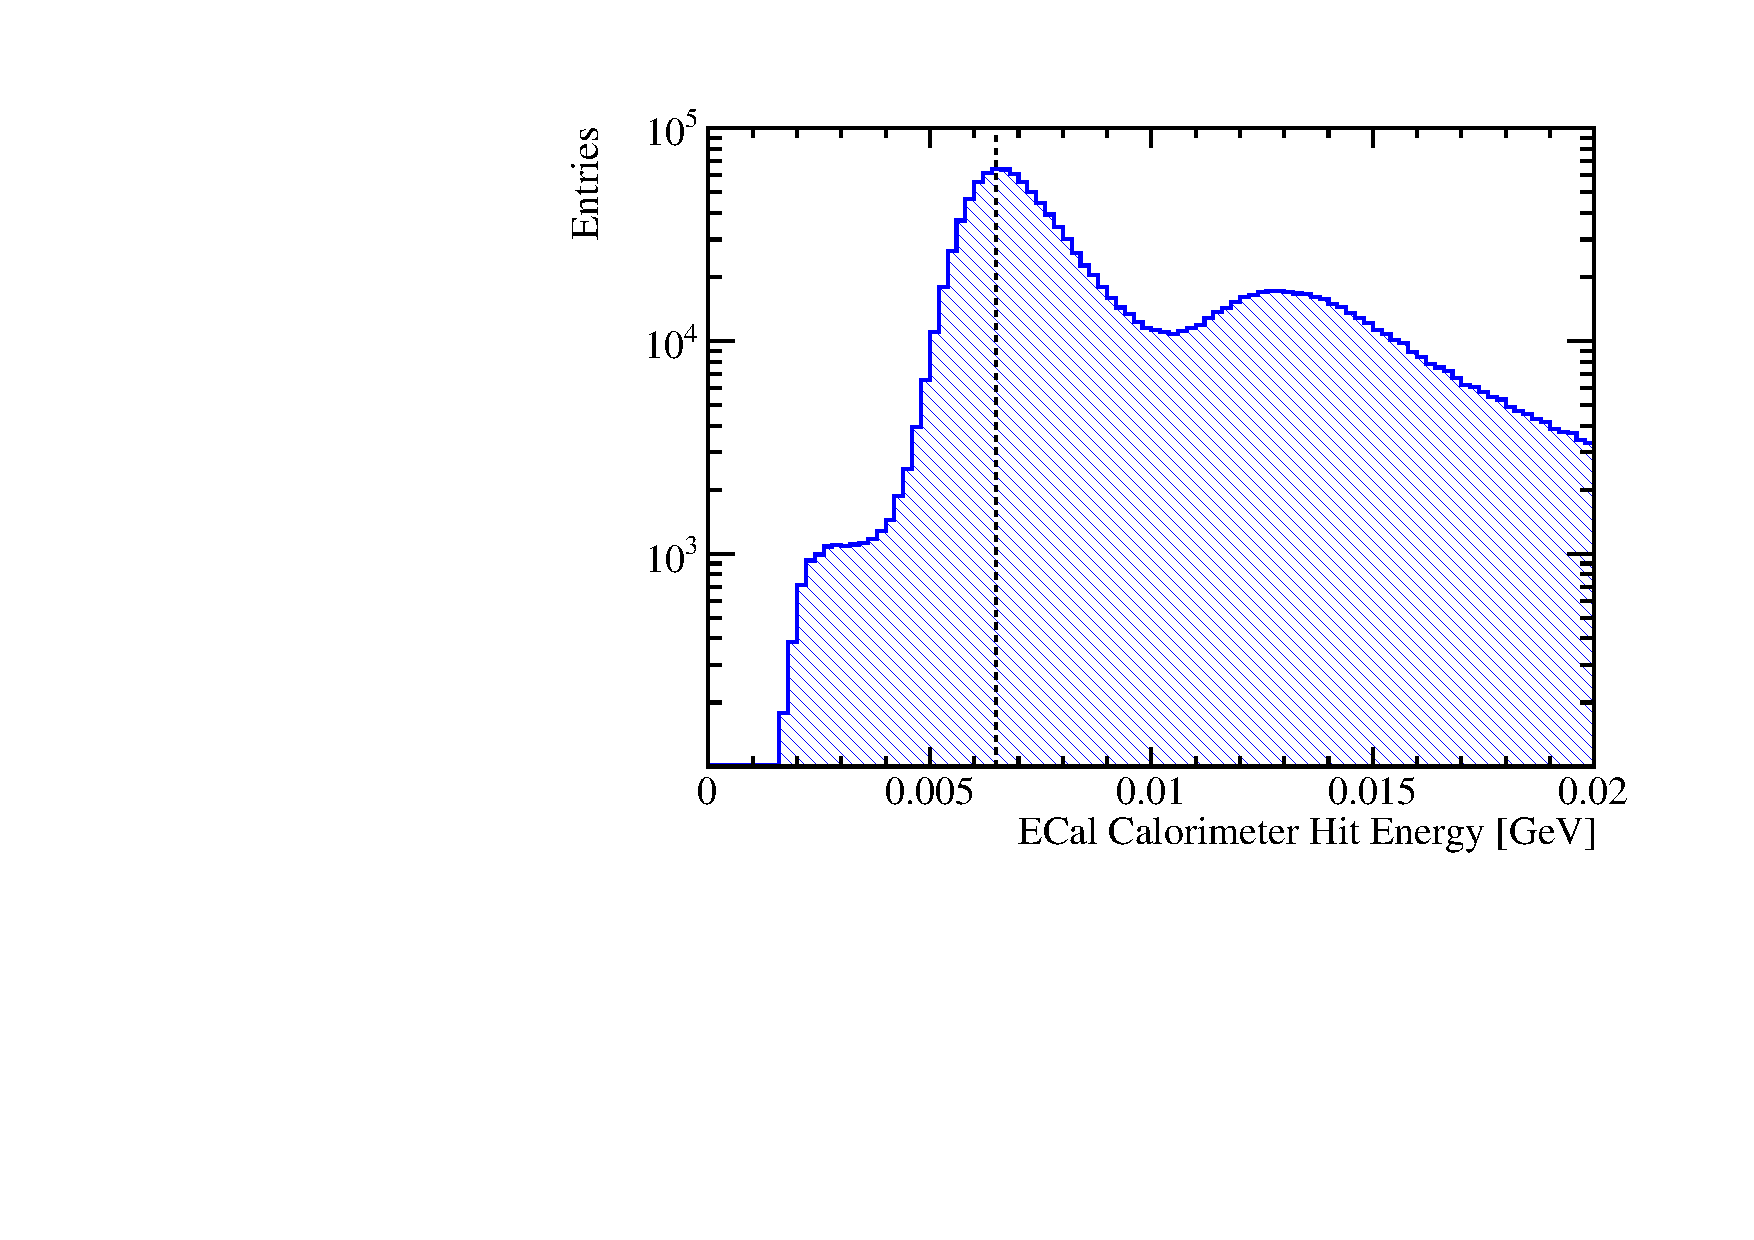
\includegraphics[width=0.5\textwidth]{EnergyEstimators/Plots/Calibration/MIPScale/PandoraPFA/MIPScalePandoraPFAECal.pdf}}
\subfloat[]{\label{fig:pandoramiphcal}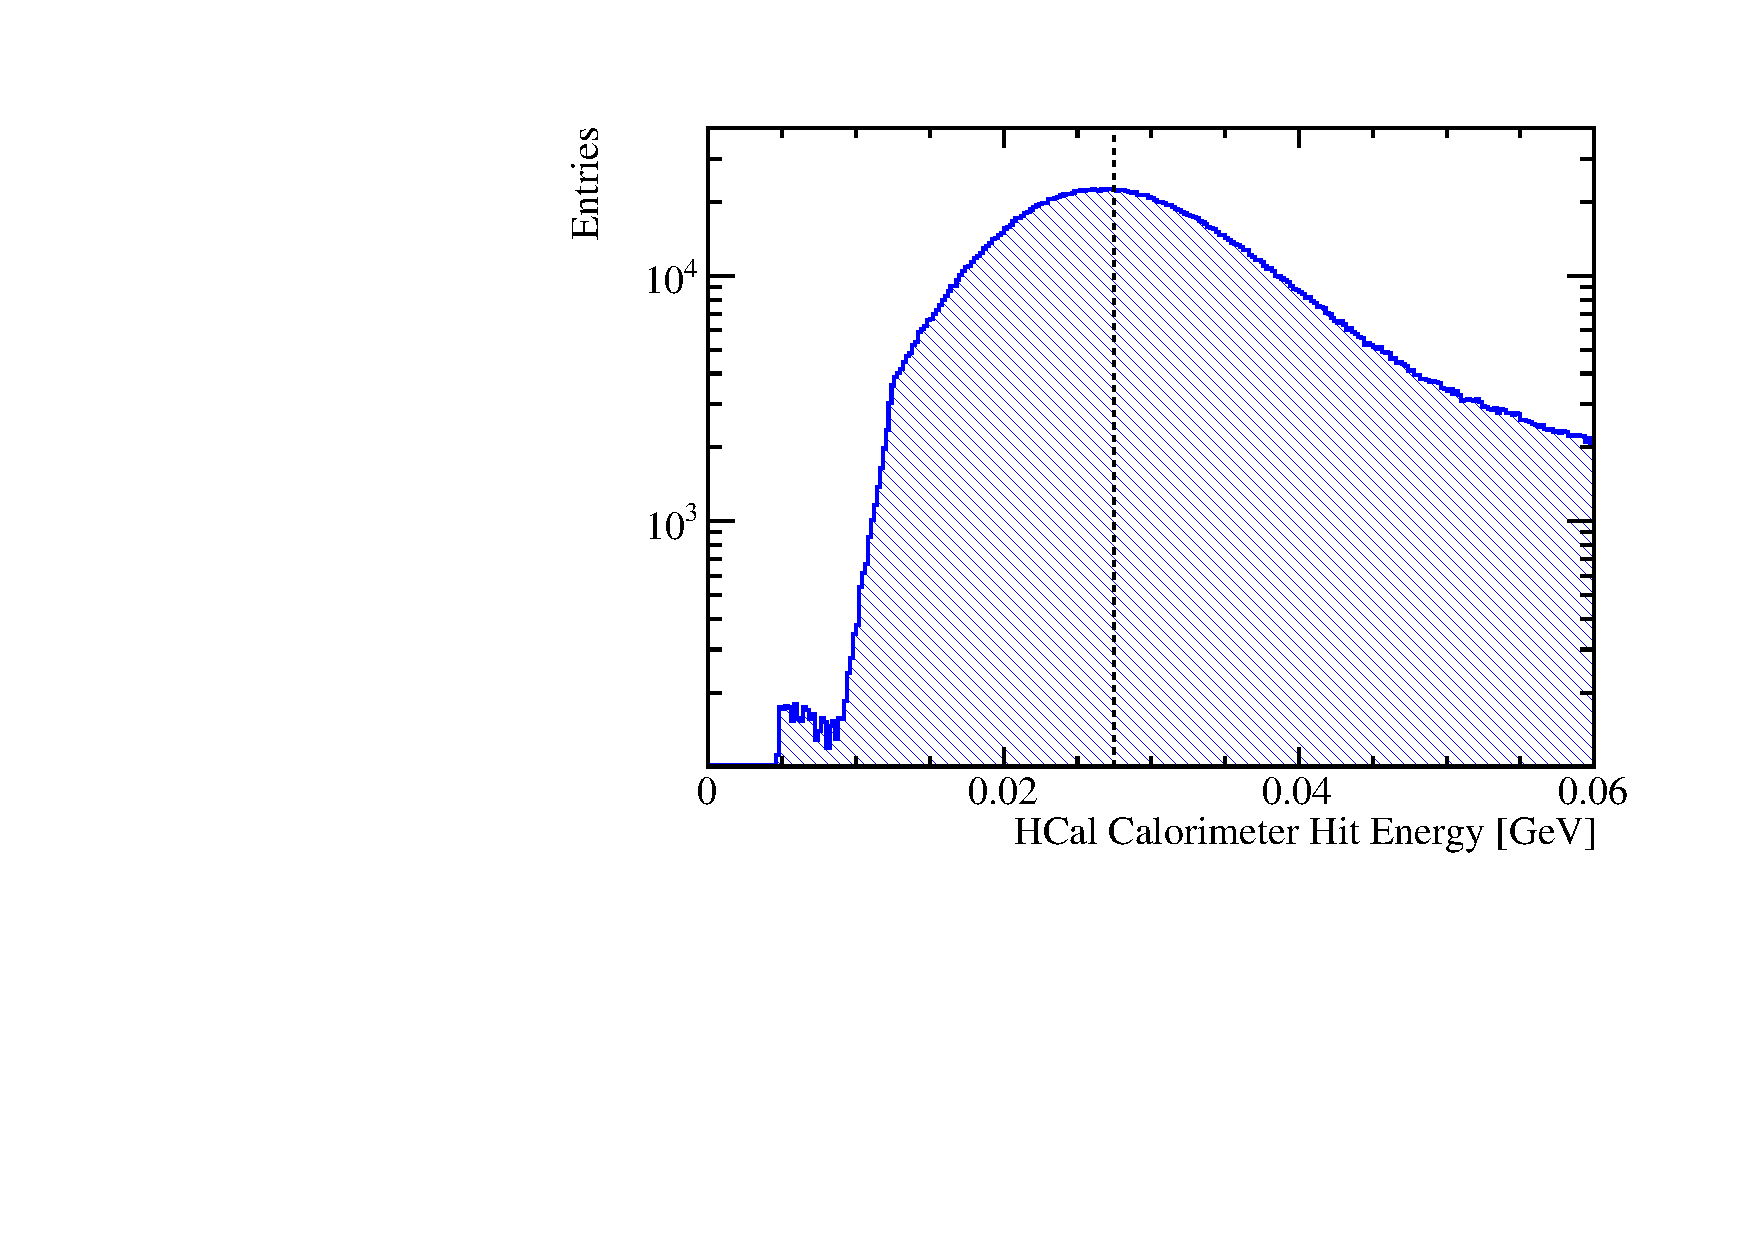
\includegraphics[width=0.5\textwidth]{EnergyEstimators/Plots/Calibration/MIPScale/PandoraPFA/MIPScalePandoraPFAHCal.pdf}} \\
\subfloat[]{\label{fig:pandoramipmuon}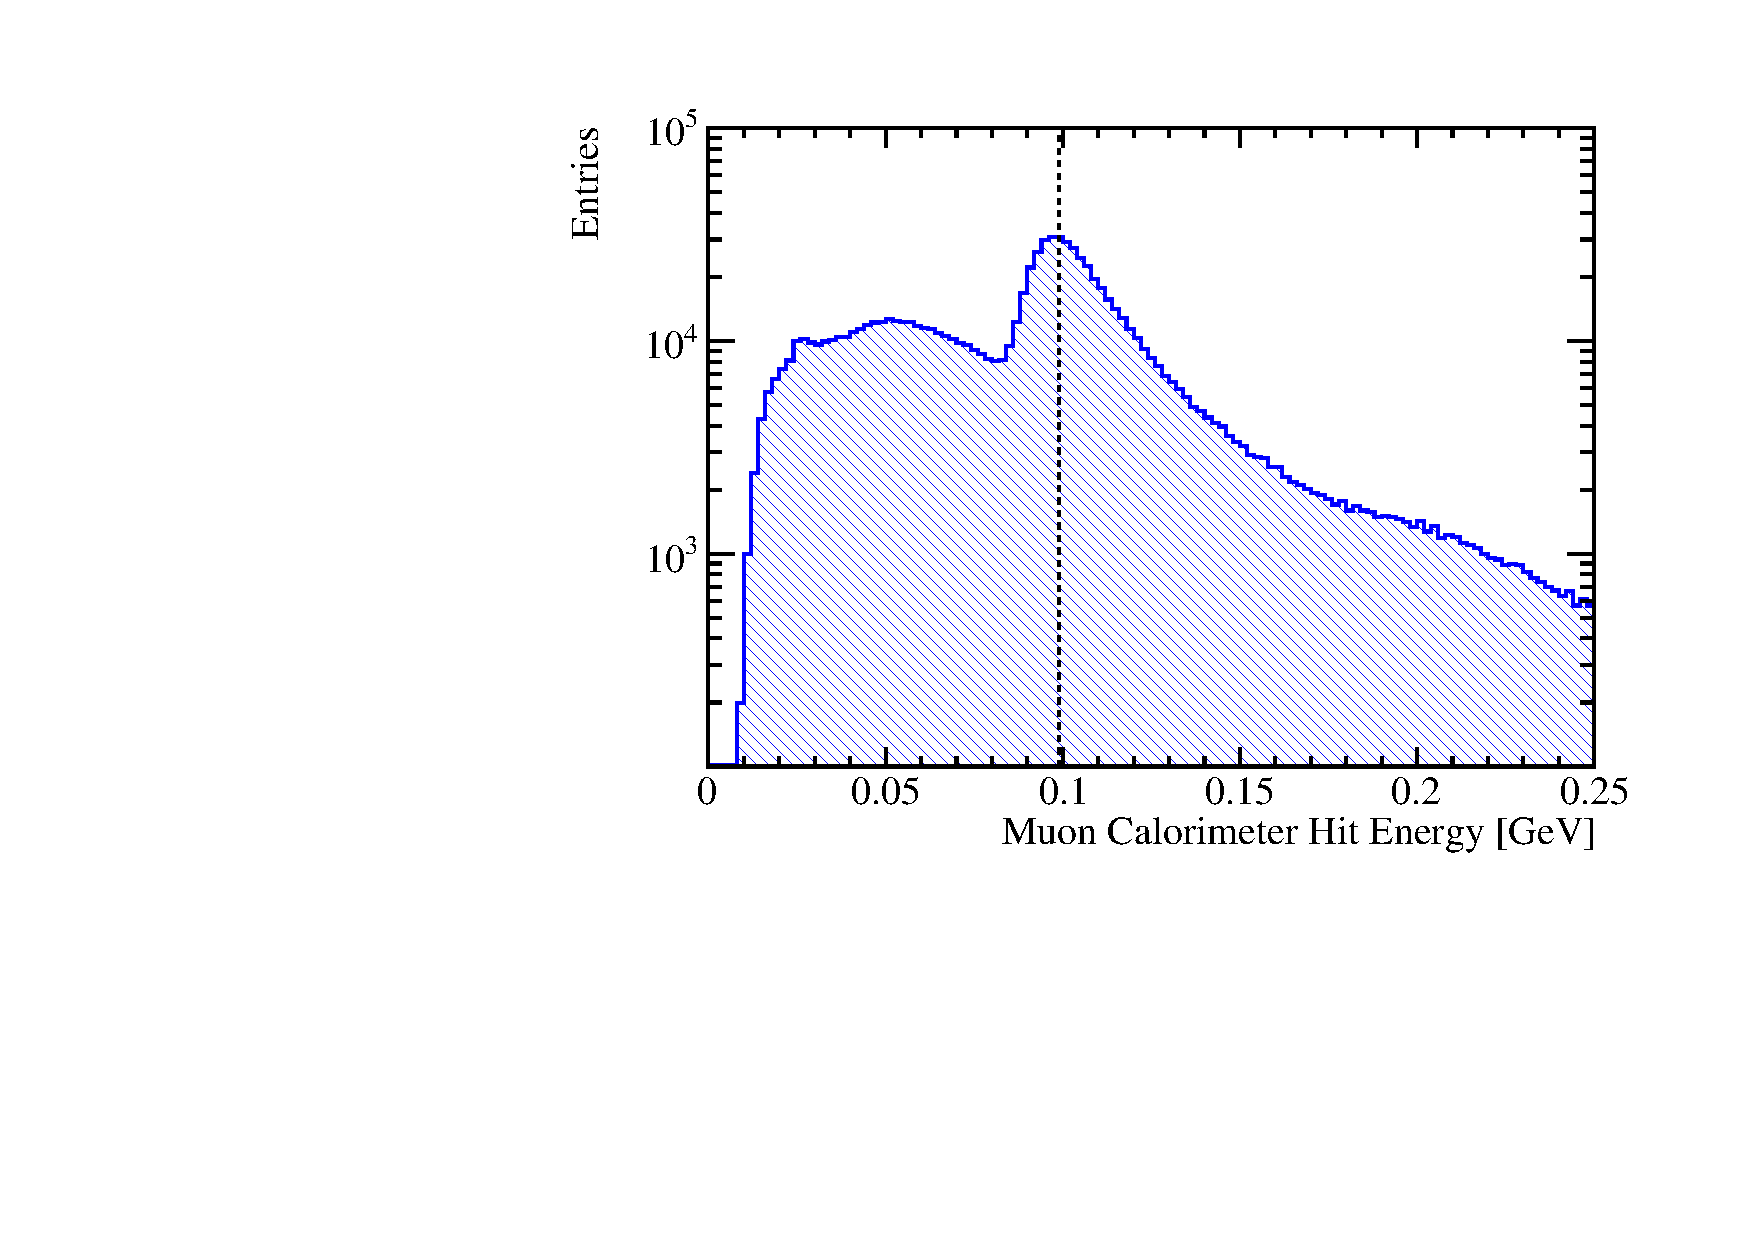
\includegraphics[width=0.5\textwidth]{EnergyEstimators/Plots/Calibration/MIPScale/PandoraPFA/MIPScalePandoraPFAMuon.pdf}}
\caption[The calorimeter hit energy distributions for \protect\subref{fig:pandoramipecal} the ECal, \protect\subref{fig:pandoramiphcal} the HCal and \protect\subref{fig:pandoramipmuon} the muon chamber for 10 GeV $\mu^{-}$ events.]{The calorimeter hit energy distributions for \protect\subref{fig:pandoramipecal} the ECal, \protect\subref{fig:pandoramiphcal} the HCal and \protect\subref{fig:pandoramipmuon} the muon chamber for 10 GeV $\mu^{-}$ events.}
\label{fig:pandoramip}
\end{figure}

%========================================================================================

\subsection{Electromagnetic and Hadronic Scale Setting}
\label{sec:scalesetting}

%========================================================================================

\subsubsection{Electromagnetic scale setting}
\label{sec:emscalesetting}
The electromagnetic scale in the ECal, $\beta^{EM}_{ECal}$, is determined using $\gamma$ events at $E_{MC} = 10$ GeV.  $\gamma$ events are ideal for the setting of the electromagnetic scale as they procedure electromagnetic showers and are primarily confined to the ECal at the energy considered, which was shown in figure \ref{fig:ecaldigiphotonsplit}.  A cut requiring less than 1\% of the reconstructed energy to be found outside the ECal is applied to ensure that only events where the bulk of the energy is deposited within the ECal are used for this part of the calibration.  Furthermore, a cut requiring a single $\gamma$ be reconstructed are added to veto events with pattern recognition failures.  $\gamma$ conversions are excluded at MC level to ensure energy measurements used in the calibration arise from the calorimeters and not the charged particle tracks.  The impact of these cuts on the electromagnetic energy measured in the ECal for 10 GeV $\gamma$ events is shown in figure \ref{fig:ecalemscaleselection}.   

The fitting procedure follows that used for the ECal digitisation, described in section \ref{sec:ecaldigi}, whereby a trial calibration for the electromagnetic energy scale in the ECal, $\beta^{EM0}_{ECal}$, is assumed and the single $\gamma$ events simulated.  The distribution of the electromagnetic energy in the ECal is created and a Gaussian fit applied to the range of data with the smallest root mean square containing at least 90 \% of the data.  The mean of this fit, $E_{\text{Fit}}$, is then used to scale $\beta^{EM0}_{ECal}$ in the following way:
%
\begin{equation}
\beta^{EM0}_{ECal} \rightarrow \beta^{EM}_{ECal} = \beta^{EM0}_{ECal} \times \frac{E_{MC}}{E_{Fit}}\text{ ,}
\end{equation}
%
An example distribution and fit used in the calibration of the nominal ILD detector model can be found in figure \ref{fig:ecalemscalefit}.  This procedure is repeated using the updated $\beta^{EM}_{ECal}$ until $E_{\text{Fit}}$ falls within a specified tolerance.  The tolerance applied here was $|E_{\text{Fit}} - E_{\text{MC}}| < E_{\text{MC}} \times 0.5 \%$.  The binning for the fitted histogram is chosen such that the bin width is equal to the desired target tolerance on $E_{\text{Fit}}$ e.g. $E_{\text{MC}} \times 0.5 \% = 0.05$ GeV.  This tolerance is tighter than was applied for the digitisation as it is these energies that are used in downstream analyses.   
 
\begin{figure}[h!]
\subfloat[]{\label{fig:ecalemscaleselection}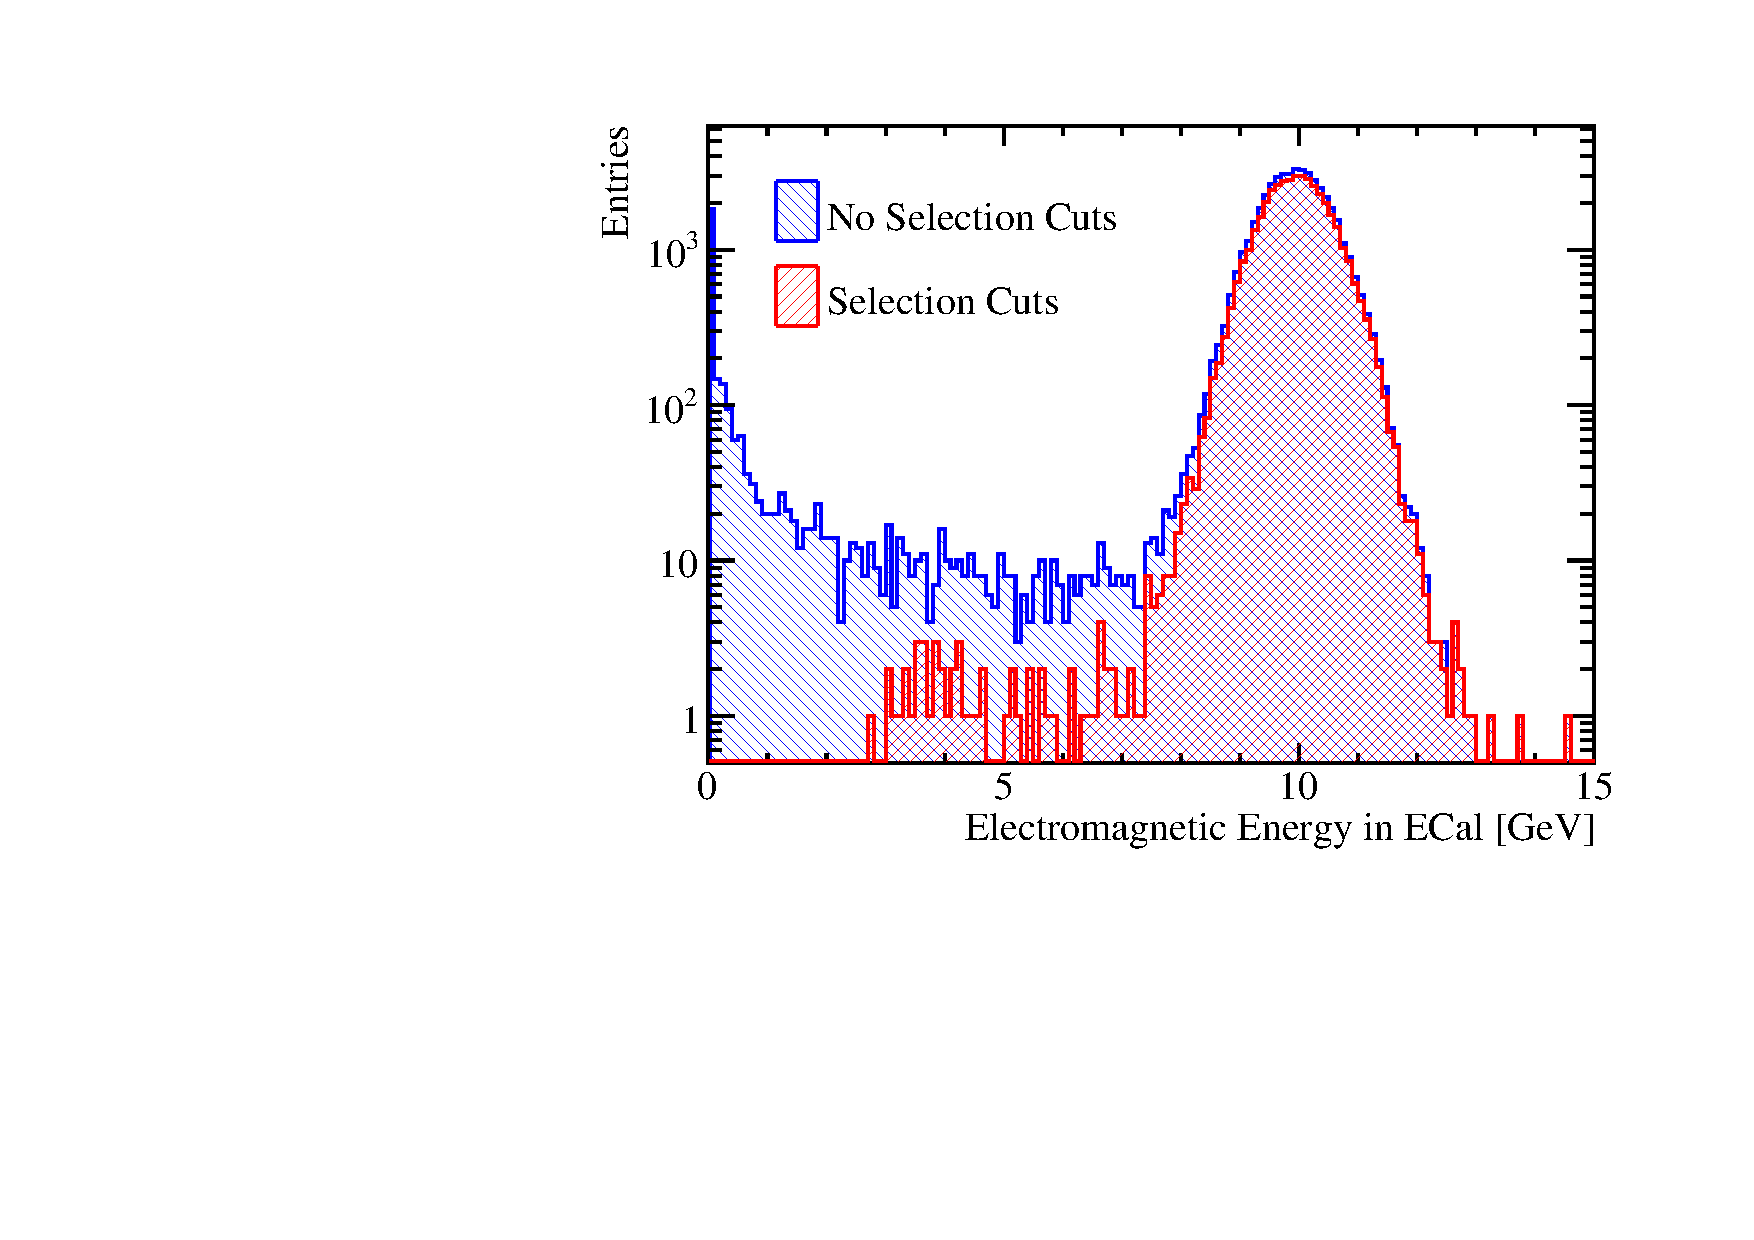
\includegraphics[width=0.5\textwidth]{EnergyEstimators/Plots/Calibration/EMScaleSetting/EMScaleECalSelection.pdf}}
\subfloat[]{\label{fig:ecalemscalefit}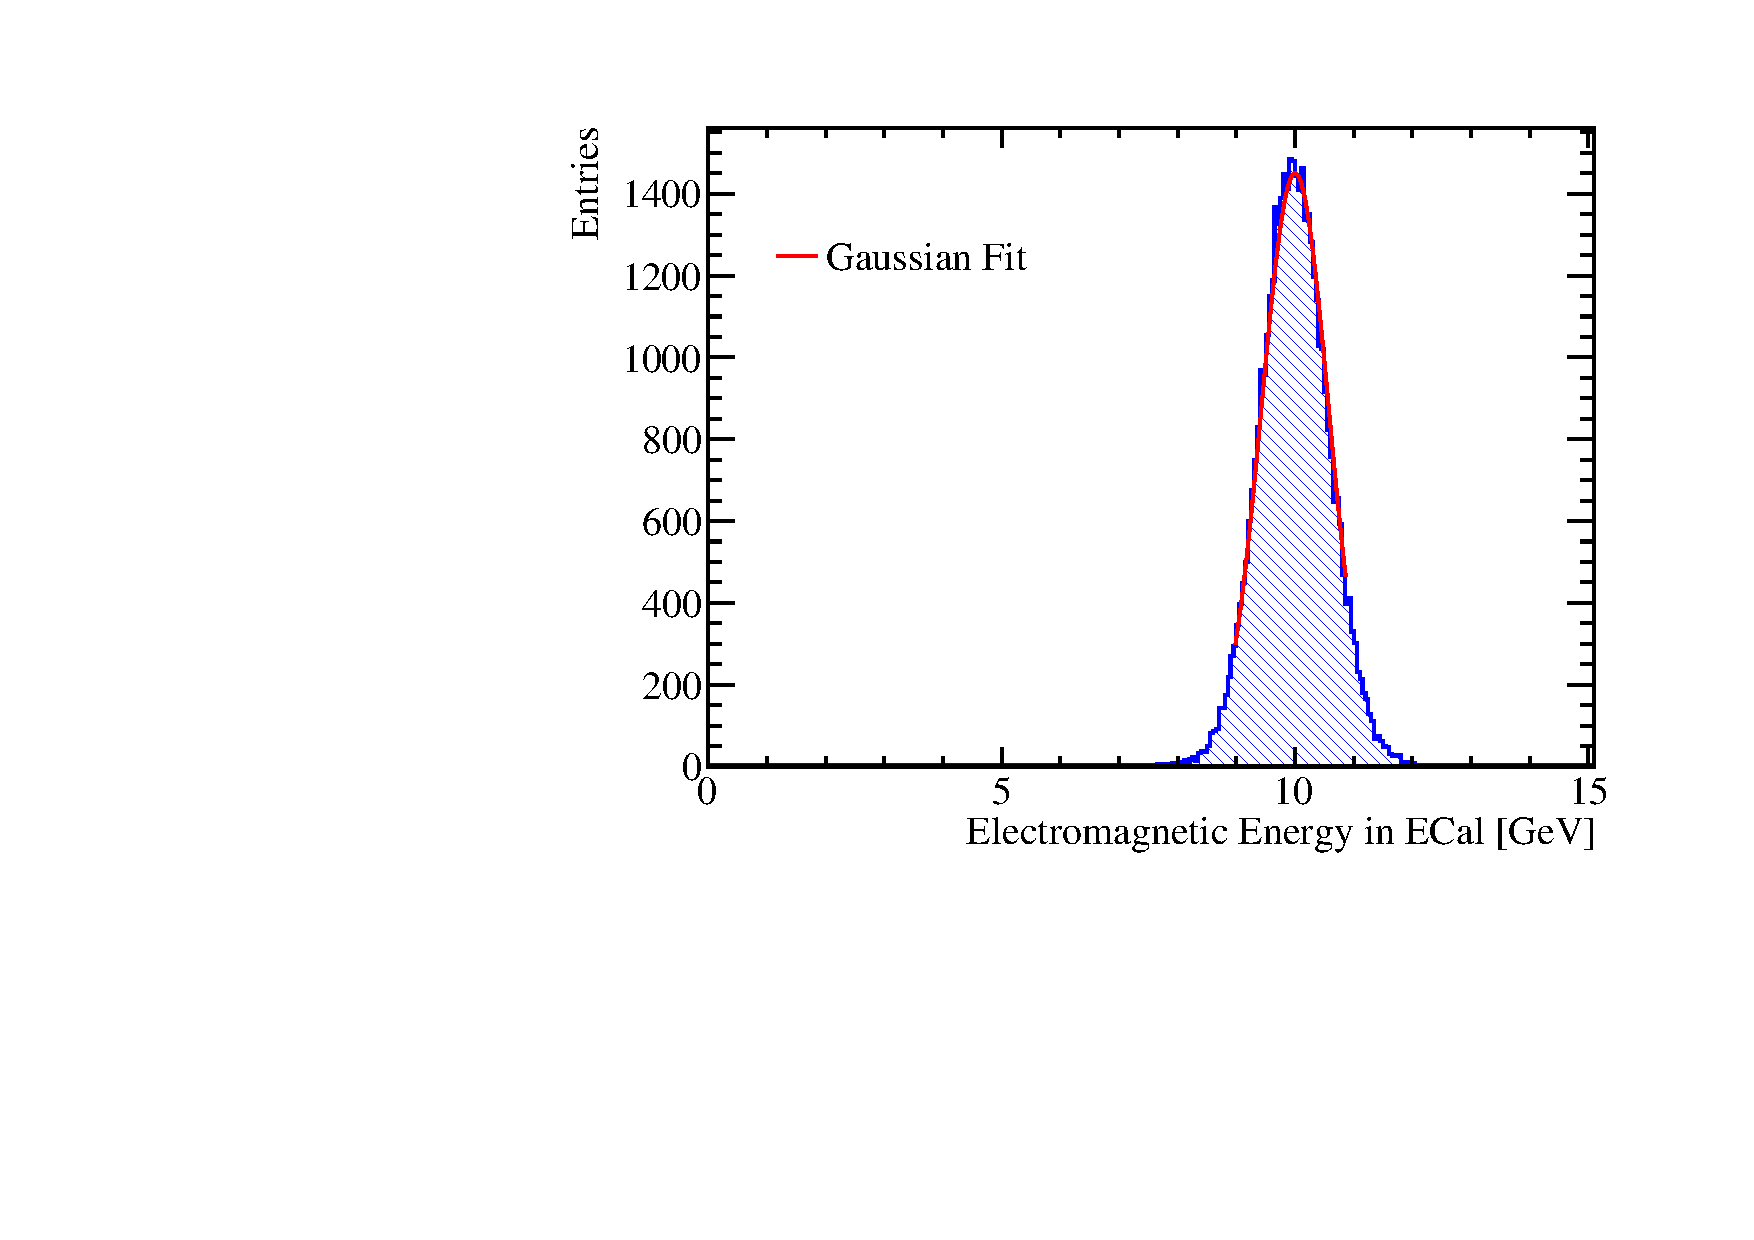
\includegraphics[width=0.5\textwidth]{EnergyEstimators/Plots/Calibration/EMScaleSetting/EMScaleSettingECalFit.pdf}}
\caption[\protect\subref{fig:ecalemscaleselection} The sum of the electromagnetic energy measured in the ECal for 10 GeV $\gamma$ events with and without the selection cuts.  \protect\subref{fig:ecalemscalefit} Gaussian fit to sum of the electromagnetic energy deposited in the ECal for 10 GeV $\gamma$ events with selection cuts.  The fine binning reflects the tolerance on the electromagnetic scale calibration constant in the ECal.]{\protect\subref{fig:ecalemscaleselection} The sum of the electromagnetic energy measured in the ECal for 10 GeV $\gamma$ events with and without the selection cuts.  \protect\subref{fig:ecalemscalefit} Gaussian fit to sum of the electromagnetic energy deposited in the ECal for 10 GeV $\gamma$ events with selection cuts.  The fine binning reflects the tolerance on the electromagnetic scale calibration constant in the ECal.}
\label{fig:ecalemscale}
\end{figure}
 
The electromagnetic scale in the HCal, $\beta^{EM}_{HCal}$, is chosen to be equal to the hadronic scale in the HCal, $\beta^{Had}_{HCal}$.  The details of the determination of $\beta^{Had}_{HCal}$ can be found in section \ref{sec:hadscalesetting}.  For the ILC and CLIC, $\beta^{EM}_{HCal}$ is not a critical parameter in the reconstruction as photons are largely contained within the ECal meaning little to no electromagnetic energy is measured in the HCal.  

%========================================================================================

\subsubsection{Hadronic scale setting}
\label{sec:hadscalesetting}
The hadronic scale in the ECal, $\beta^{Had}_{ECal}$, is important to detector performance as a non-negligible amount of hadronic energy will be measured in the ECal.  As the ECal contains $\approx 1 \lambda_{I}$, the hadronic scale in the ECal cannot be independently set as it is unfeasible to create a large sample of 20 GeV $K^{0}_{L}$ events that are fully contained within it.  Therefore, the hadronic scale in the ECal and HCal have to be set simultaneously.  Cuts are applied to select the $K^{0}_{L}$ events that are appropriate to use for the hadronic scale calibration.  To ensure the events do not suffer from the effect of leakage out of the back of the HCal, a cut is applied requiring the last layer in which energy is deposited in the HCal to be in the first 90\% of the HCal.  In addition to this, a cut requiring a single neutral hadron to be reconstructed is applied to veto events with reconstruction failures.  Finally, the total hadronic energy measured in ECal and HCal, $E^{Had}_{ECal} + E^{Had}_{HCal}$, must fall within 3 $\sigma$ of the desired hadronic energy distribution, $E^{Had}_{ECal} + E^{Had}_{HCal} = 20 \text {GeV} - m_{K^{0}_{L}} = E_{K}$.  Where $\sigma$ is defined to be $55\% \times \sqrt{E} = 2.46 \text{GeV}$ for 20 GeV $K^{0}_{L}$.  This definition for $\sigma$ is derived from the energy resolution for neutral hadrons using the nominal ILD HCal \cite{Behnke:2013lya}.  This cut ensures that when fitting the two dimensional distribution of hadronic energy measured in the ECal and HCal outliers do not skew the fit.  Again, the target reconstructed energy for this sample is the kinetic energy and not the total energy of the $K^{0}_{L}$ for the reasons outlined in section \ref{sec:hcaldigi}.  The impact of cuts are illustrated in figure \ref{fig:hadscaleselection}.

\begin{figure}[h!]
\subfloat[]{\label{fig:hadscaleselectionnocuts}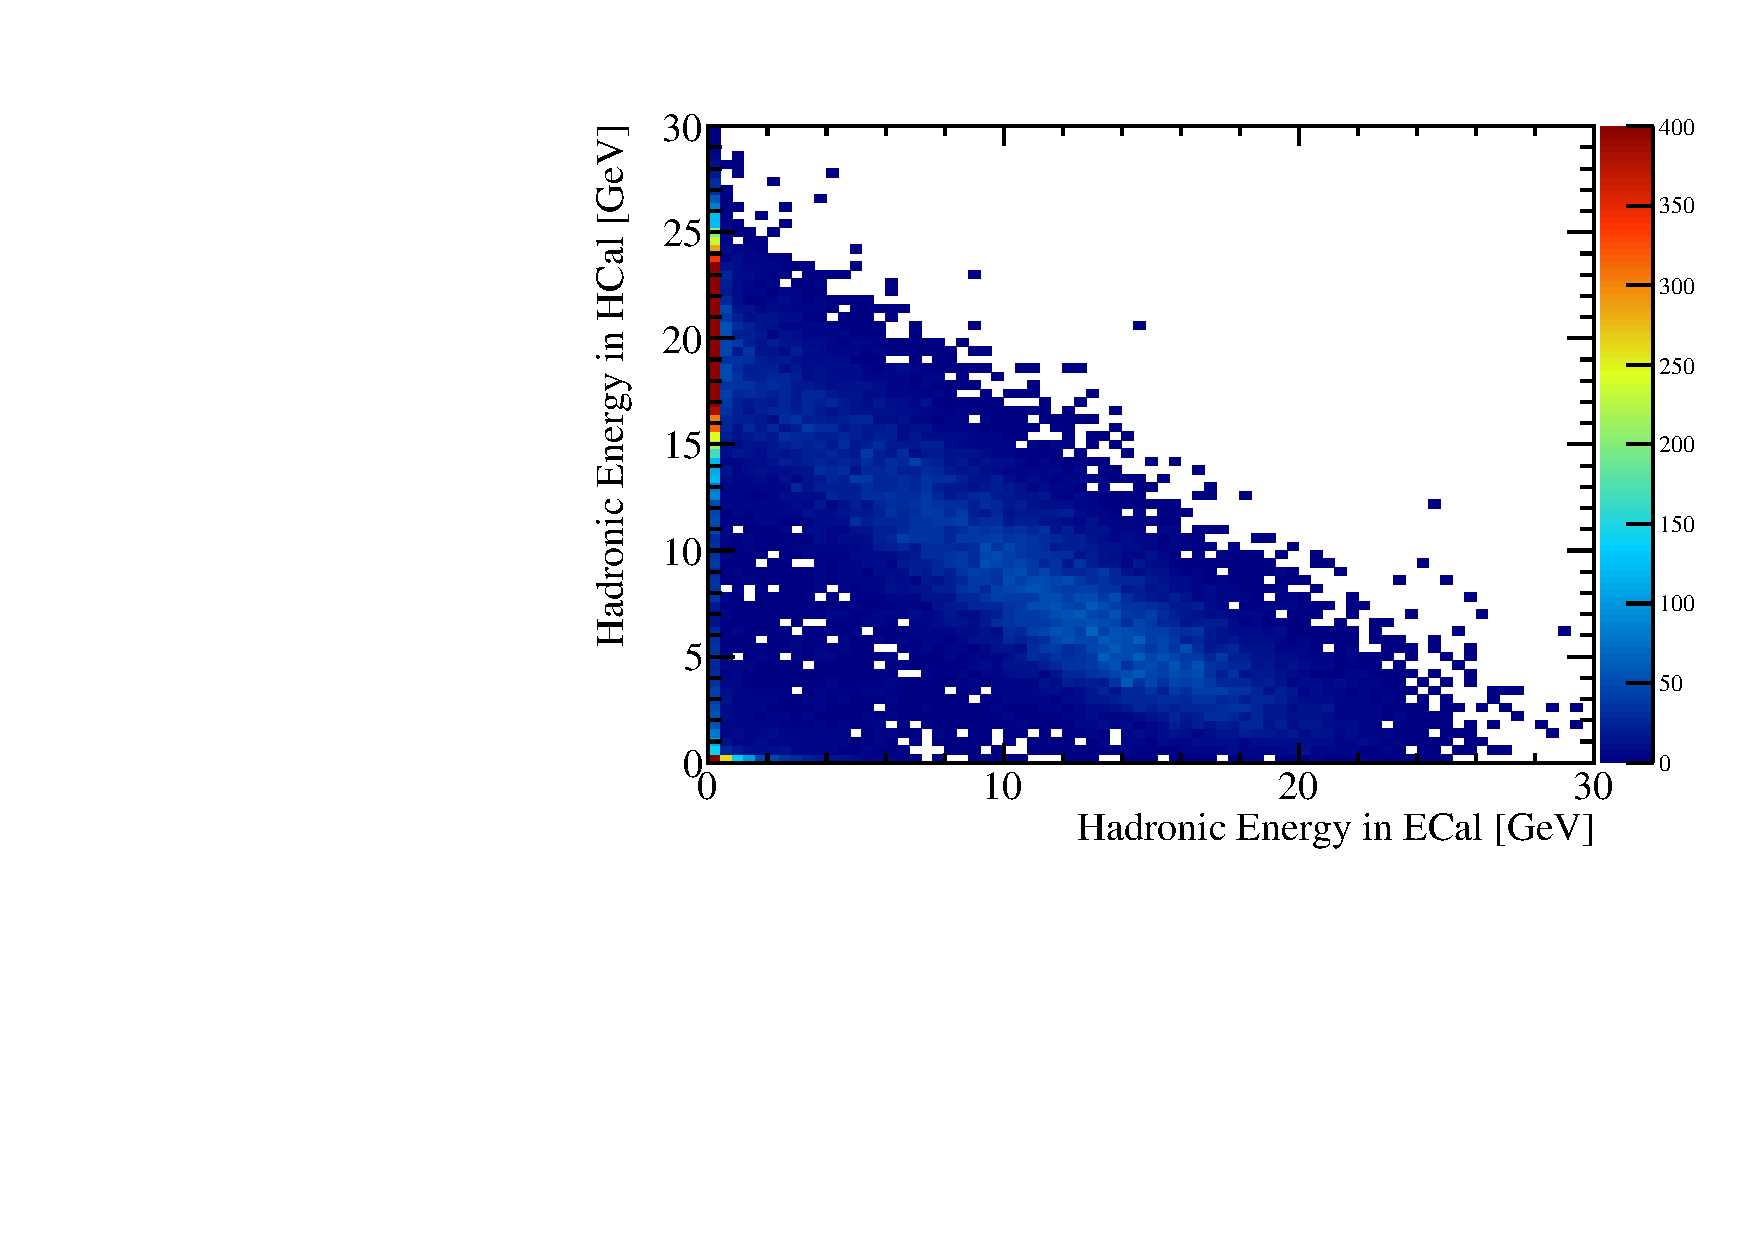
\includegraphics[width=0.5\textwidth]{EnergyEstimators/Plots/Calibration/HadScaleSetting/HadScaleECalHCalSelectionNoCuts.pdf}}
\subfloat[]{\label{fig:hadscaleselectioncuts}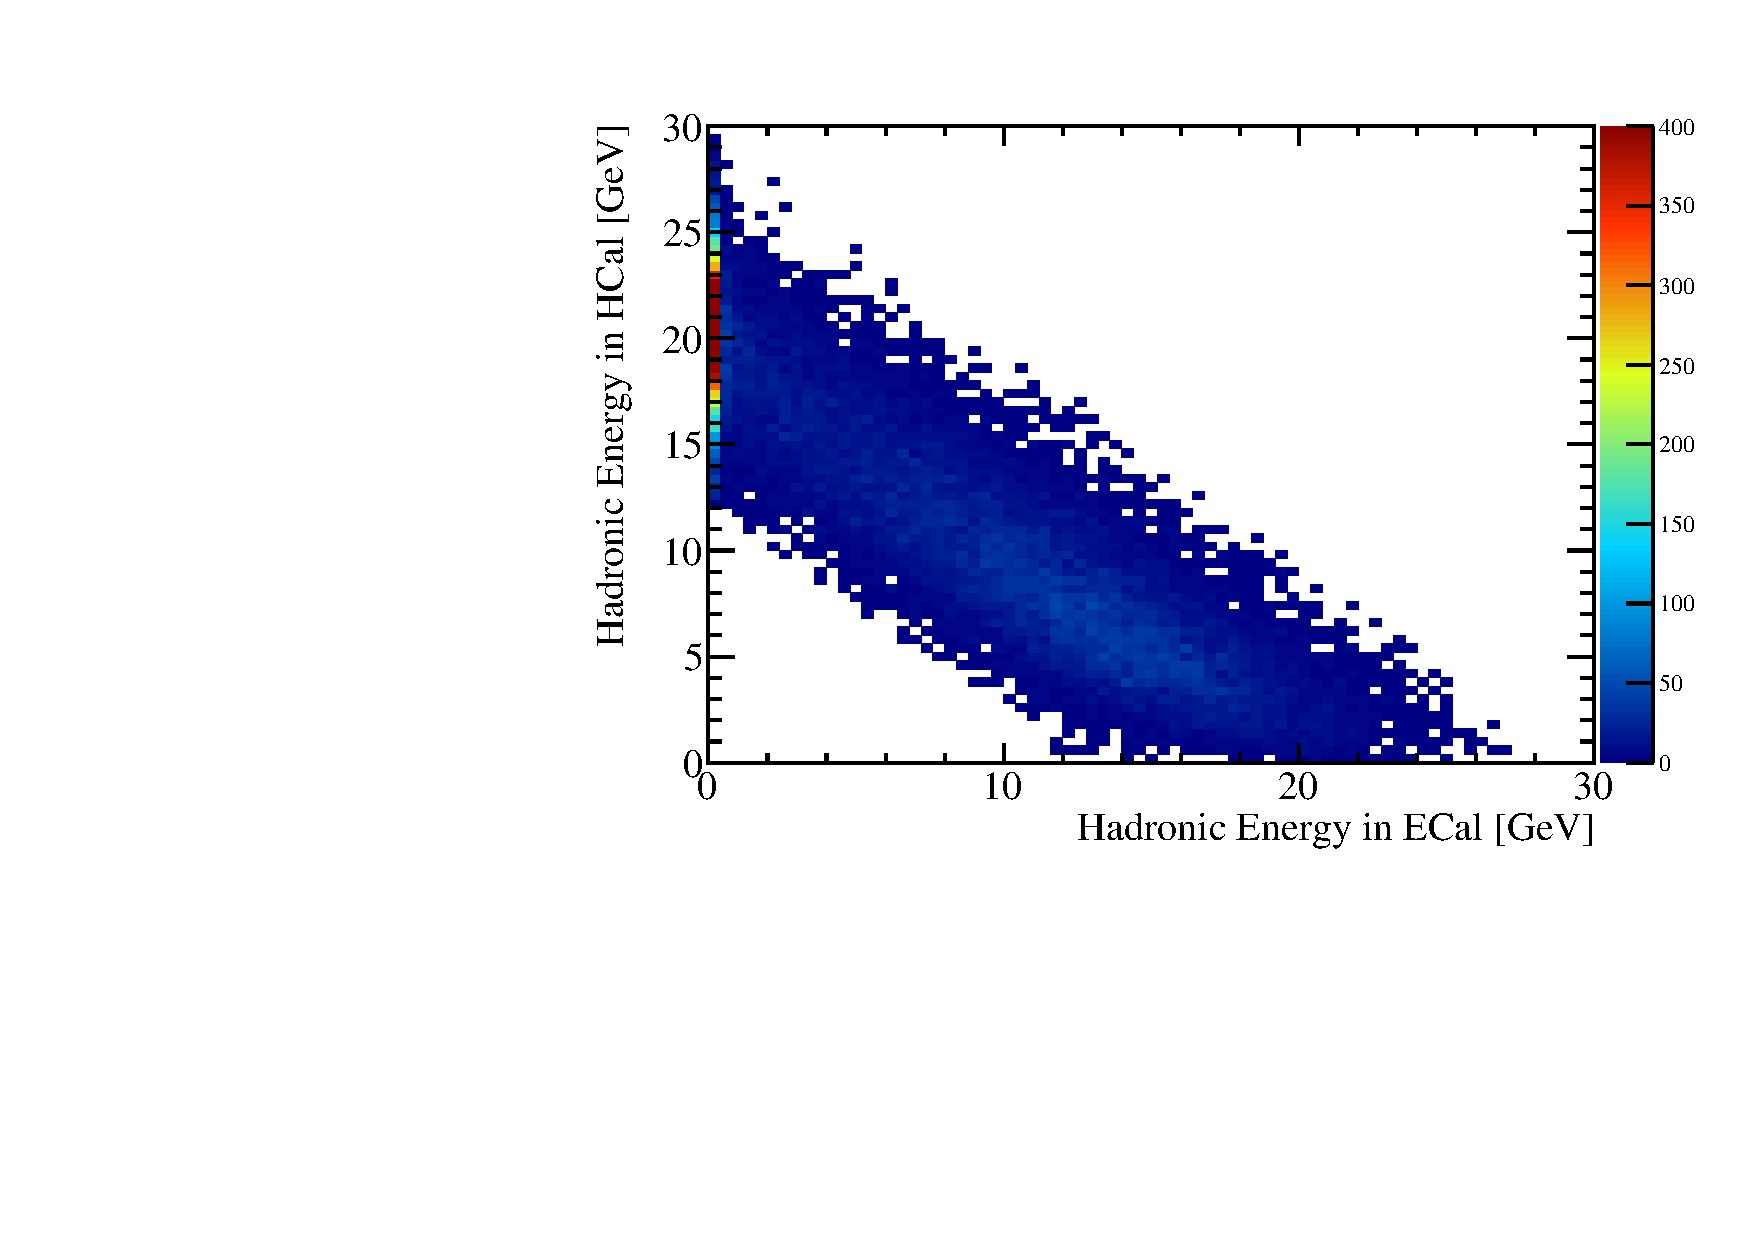
\includegraphics[width=0.5\textwidth]{EnergyEstimators/Plots/Calibration/HadScaleSetting/HadScaleECalHCalSelectionCuts.pdf}}
\caption[The distribution of hadronic energy measured in the ECal and HCal for 20 GeV $K^{0}_{L}$ events with and without selection cuts.]{The distribution of hadronic energy measured in the ECal and HCal for 20 GeV $K^{0}_{L}$ events \protect\subref{fig:hadscaleselectionnocuts} without selection cuts and \protect\subref{fig:hadscaleselectioncuts} with selection cuts.}
\label{fig:hadscaleselection}
\end{figure}

This part of the calibration procedure is again iterative and begins by assuming trial values, $\beta^{Had0}_{ECal}$ and $\beta^{Had0}_{ECal}$, for the hadronic scale calibration factors $\beta^{Had}_{ECal}$ and $\beta^{Had}_{ECal}$.  The 20 GeV $K^{0}_{L}$ events are then simulated and reconstructed.  Following that a linear fit to the distribution of $E^{Had}_{ECal}$ against $E^{Had}_{HCal}$ for 20 GeV $K^{0}_{L}$ events passing the selection cuts is applied.  The fit is performed by minimising $\chi^{2}$, which is defined as:
%
\begin{equation}
\chi^{2}(\delta^{Had}_{ECal}, \delta^{Had}_{HCal}) = \sum_{i} \frac{x_{i}}{\sigma_{x_{i}}}\text{ ,}
\end{equation}
%
\noindent where $x_{i}$ is the perpendicular distance from $E^{Had}_{ECal}$ and $E^{Had}_{HCal}$ for event $i$ to the line $E^{Had}_{HCal} = \delta^{Had}_{HCal} - E^{Had}_{ECal} \frac{\delta^{Had}_{HCal}}{\delta^{Had}_{ECal}}$.   The definition of $x_{i}$ is given in equation \ref{equ:xicalc}, but best illustrated by considering figure \ref{fig:hadscalechi2calc}.  $\sigma_{x_{i}}$ is the uncertainty on $x_{i}$, which is calculated by propagating the uncertainties on $E^{Had}_{ECal}$ and $E^{Had}_{HCal}$, which are assumed to be $\sigma_{E^{Had}_{E/HCal}} = 55\% \times \sqrt{E^{Had}_{E/HCal}}$, into the expression for $x_{i}$.  The result of this propagation of errors is given in equation \ref{equ:sigmaxicalc}.  The sum runs over all events, $i$, passing the selection cuts.  
%
\begin{equation}
x_{i} = \frac{E^{Had}_{HCal} \delta^{Had}_{ECal} + E^{Had}_{ECal} \delta^{Had}_{HCal} - \delta^{Had}_{ECal} \delta^{Had}_{HCal}}{\sqrt{(\delta^{Had}_{ECal})^{2} + (\delta^{Had}_{HCal})^{2}}}\text{ ,}
\label{equ:xicalc}
\end{equation}
\begin{equation}
\sigma_{i} = \frac{(\sigma_{E^{Had}_{HCal}}  \delta^{Had}_{ECal})^{2} + (\sigma_{E^{Had}_{ECal}} \delta^{Had}_{HCal})^{2}}{\sqrt{(\delta^{Had}_{ECal})^{2} + (\delta^{Had}_{HCal})^{2}}}\text{ ,}
\label{equ:sigmaxicalc}
\end{equation}
%
\begin{figure}[h!]
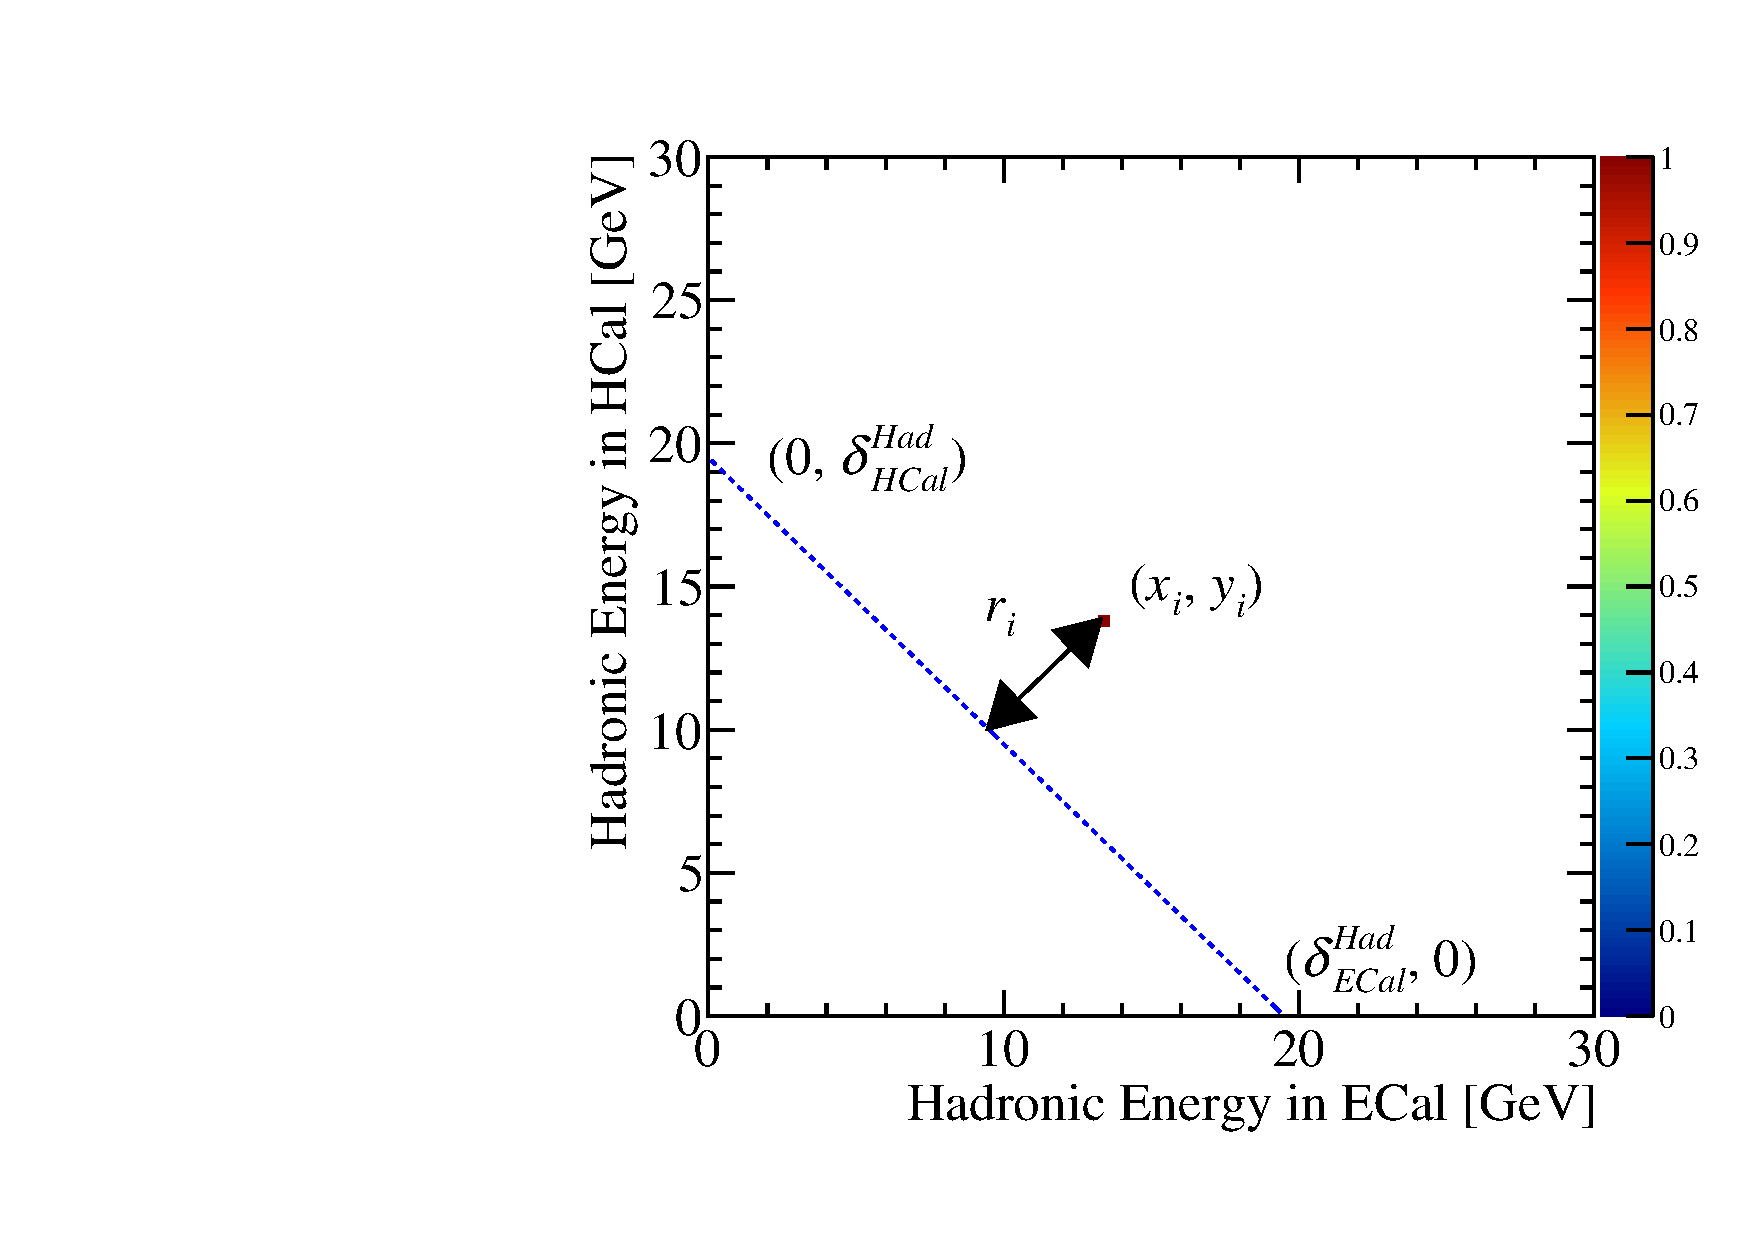
\includegraphics[width=0.5\textwidth]{EnergyEstimators/Plots/Calibration/HadScaleSetting/HadScaleECalHCalSelectionExample.pdf}
\caption[An example showing the definition of $x_{i}$, the variable used for the calculation of $\chi^{2}(\delta^{Had}_{ECal}, \delta^{Had}_{HCal})$ for the setting of the hadronic energy scale.]{An example showing the definition of $x_{i}$, the variable used for the calculation of $\chi^{2}$ for the setting of the hadronic energy scale.  For an event that has been measured with hadronic energy $E^{Had}_{ECal}$ in the ECal and $E^{Had}_{HCal}$ in the HCal, the geometric interpretation of $x_{i}$ is shown.  The blue dotted line is defined as $E^{Had}_{HCal} = \delta^{Had}_{HCal} - E^{Had}_{ECal} \frac{\delta^{Had}_{HCal}}{\delta^{Had}_{ECal}}$.}
\label{fig:hadscalechi2calc}
\end{figure}

The minimisation of $\chi^{2}$ is done by stepping over a range of $\delta^{Had}_{ECal}$ and $\delta^{Had}_{HCal}$ centred about the ideal value of $20 \text { GeV} - m_{K^{0}_{L}}$ in search for the minimum $\chi^{2}$.  Once the minima in $\chi^{2}$ is found the trial calibration factors $\beta^{Had0}_{ECal}$ and $\beta^{Had0}_{ECal}$ are rescaled to correct for any deviation from the desired fit as follows:
%
\begin{equation}
\beta^{Had0}_{ECal} \rightarrow \beta^{Had}_{ECal} = \beta^{Had0}_{ECal} \times \frac{E_{K}}{\Delta^{Had}_{ECal}} \text{ ,}\\
\beta^{Had0}_{HCal} \rightarrow \beta^{Had}_{HCal} = \beta^{Had0}_{HCal} \times \frac{E_{K}}{\Delta^{Had}_{HCal}}\text{ ,}
\end{equation}
%
\noindent where $\Delta^{Had}_{ECal}$ and $\Delta^{Had}_{ECal}$ are the values of $\delta^{Had}_{ECal}$ and $\delta^{Had}_{ECal}$ giving the minimum $\chi^{2}$.  The step sizes used for minimising $\chi^{2}$ with respect to $\delta^{Had}_{ECal}$ and $\delta^{Had}_{ECal}$ is chosen such that a single step corresponds to the target final tolerance on $\delta^{Had}$ i.e. $|\delta^{Had}_{E/HCal} - E_{\text{MC}}| < E_{\text{MC}} \times 0.5 \% \approx 0.1 \text{GeV}$.  This procedure is then repeated until $\Delta^{Had}_{ECal}$ and $\Delta^{Had}_{ECal}$ both fall within a given tolerance, which in this case it taken to be $|\Delta^{Had}_{E/HCal} - E_{\text{MC}}| < E_{\text{MC}} \times 0.5 \% \approx 0.1 \text{GeV}$.

%========================================================================================

\subsection{Retraining photon likelihood data}
The likelihood data used by PandoraPFA in the identification of electromagnetic showers is trained using off-shell mass Z boson (Z') events at 500 GeV decaying into light quarks (u, d, s).  It is necessary to retrain this data only when varying the ECal as electromagnetic showers are largely contained within the ECal at the energies being considered and the likelihood data only uses measurements made in the ECal.

As this data uses post digitisation hits it is important to ensure that a fully calibrated detector is used when retraining the likelihood data.  Therefore, it is necessary to run the calibration procedure, as described in section \ref{sec:orderingcalib}, before retaining.  However, as the reconstruction uses likelihood data the calibration procedure must be performed twice.  Initially the calibration procedure is performed where PandoraPFA is run without the inclusion of this likelihood data, using PandoraSettingsMuon.xml.  Then the likelihood data is retrained using the results of the first calibration pass and then the retrained likelihood data is used in the second pass of the calibration procedure.  

%========================================================================================
%========================================================================================

\section{Novel Energy Estimators}
This section focuses upon novel energy estimators, introduced in section \ref{sec:motivation}.  Both techniques modify the cluster energy estimator by introducing weights, $\omega^{i}$, to energy deposits in the HCal that vary as a function of energy:
%
\begin{equation}
E_{Cluster} & = \sum_{ECal \text{ } hits \text{, }i} E^{i}_{ECal} +\sum_{HCal \text{ } hits \text{, }i} E^{i}_{HCal} \omega^{i} \text{ ,}
\label{equ:compensation}
\end{equation}
%
\noindent As hadronic showers are largely contained in the HCal, weights are only applied to HCal hits.  The weights $\omega^{i}$ vary a function of the hit energy density $\rho^{i} = \frac{E^{i}_{HCal}}{V}$, where $V$ is the HCal hit volume, and, while the exact weight values depend on the implementation of the technique, a general feature present in both is that at large $E^{i}_{HCal}$ the weight is less than one.  This reduces the energy of spuriously high energy cells to limit the impact of Landau fluctuations.  The metrics used for quantifying detector performance when using these novel energy estimators are thoroughly defined in chapter \ref{chap:detopt}.

%========================================================================================

\subsection{HCal Hit Energy Truncation}
\label{sec:hcalcelltruncation}
\subsubsection{Application}
The first technique to be examined is a simple truncation of the hadronic energy recorded in any given HCal hit.  This improves the energy estimators for hadronic clusters by limiting the impact of Landau fluctuations.  In terms of $\omega$ introduced in equation \ref{equ:compensation} the truncation corresponds to:
%
\begin{equation}
\omega(\rho) =
\begin{cases}
1 & \text{if } \rho \times V < \kappa \text{ ,} \\
\frac{\kappa}{\rho \times V} & \text{otherwise} \text{ ,}
\end{cases}
\end{equation}
%
\noindent where $\kappa$ is the value of the truncation and $V$ is the volume of a HCal hit.  This weight as a function of hit energy density is shown in figure \ref{fig:hcalcellweight}.  

%========================================================================================

\subsubsection{Results: Energy Resolution}

The application of these weights can lead to improvements in the energy resolution for neutral hadrons, which can be seen in figure \ref{fig:ercelltrunckaons}.  However, a great deal of care has to be given to the truncation energy so that hits from typical hadronic shower development are not truncated, while the spuriously high energy hits are.  Figure \ref{fig:ercelltrunckaons} indicates that a 1~GeV truncation is sufficient for dealing with the Landau fluctuations.  For hit energy truncations greater than this the energy resolution worsens as the effect Landau fluctuations are not accounted for, while for hit energy truncations below 1~GeV the truncation is too aggressive and hits from typical hadronic shower development are truncated.  For completion the $\gamma$ energy resolutions as a function of HCal hit energy truncation are shown in figure \ref{fig:ercelltruncphotons}.  As expected the $\gamma$ energy resolution is invariant to the HCal hit energy truncation as the $\gamma$s are largely contained within the ECal.

\begin{figure}[h!]
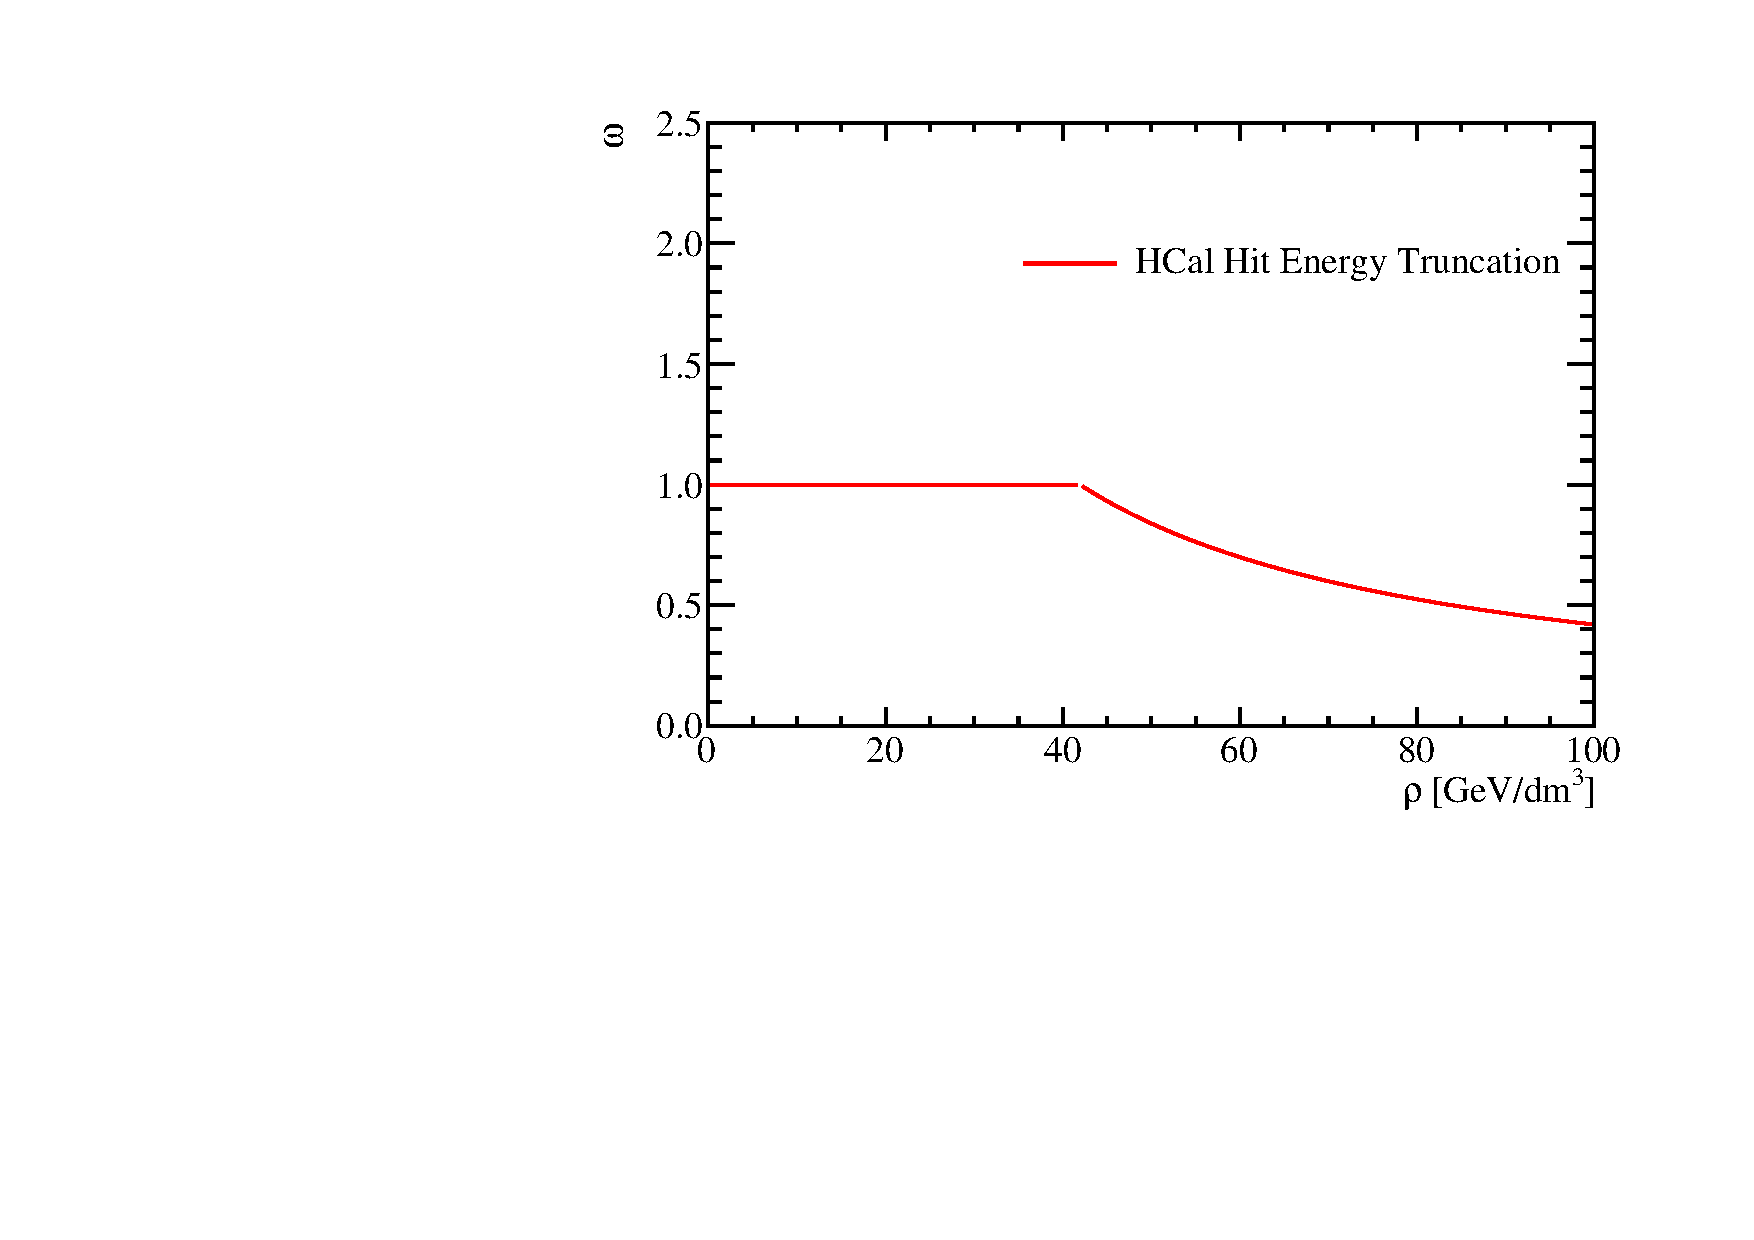
\includegraphics[width=0.5\textwidth]{EnergyEstimators/Plots/SoftComp/Weights/CellTruncWeights.pdf}
\caption[The weights, $\omega$, used in the HCal hit energy truncation as a function of the energy density of the HCal hit, $\rho$.  The truncation shown here corresponds to a 1~GeV truncation in the nominal ILD HCal.]{The weights, $\omega$, used in the HCal hit energy truncation as a function of the energy density of the HCal hit, $\rho$.  The truncation shown here corresponds to a 1~GeV truncation in the nominal ILD HCal.}
\label{fig:hcalcellweight}
\end{figure}

\begin{figure}[h!]
\subfloat[]{\label{fig:ercelltrunckaons}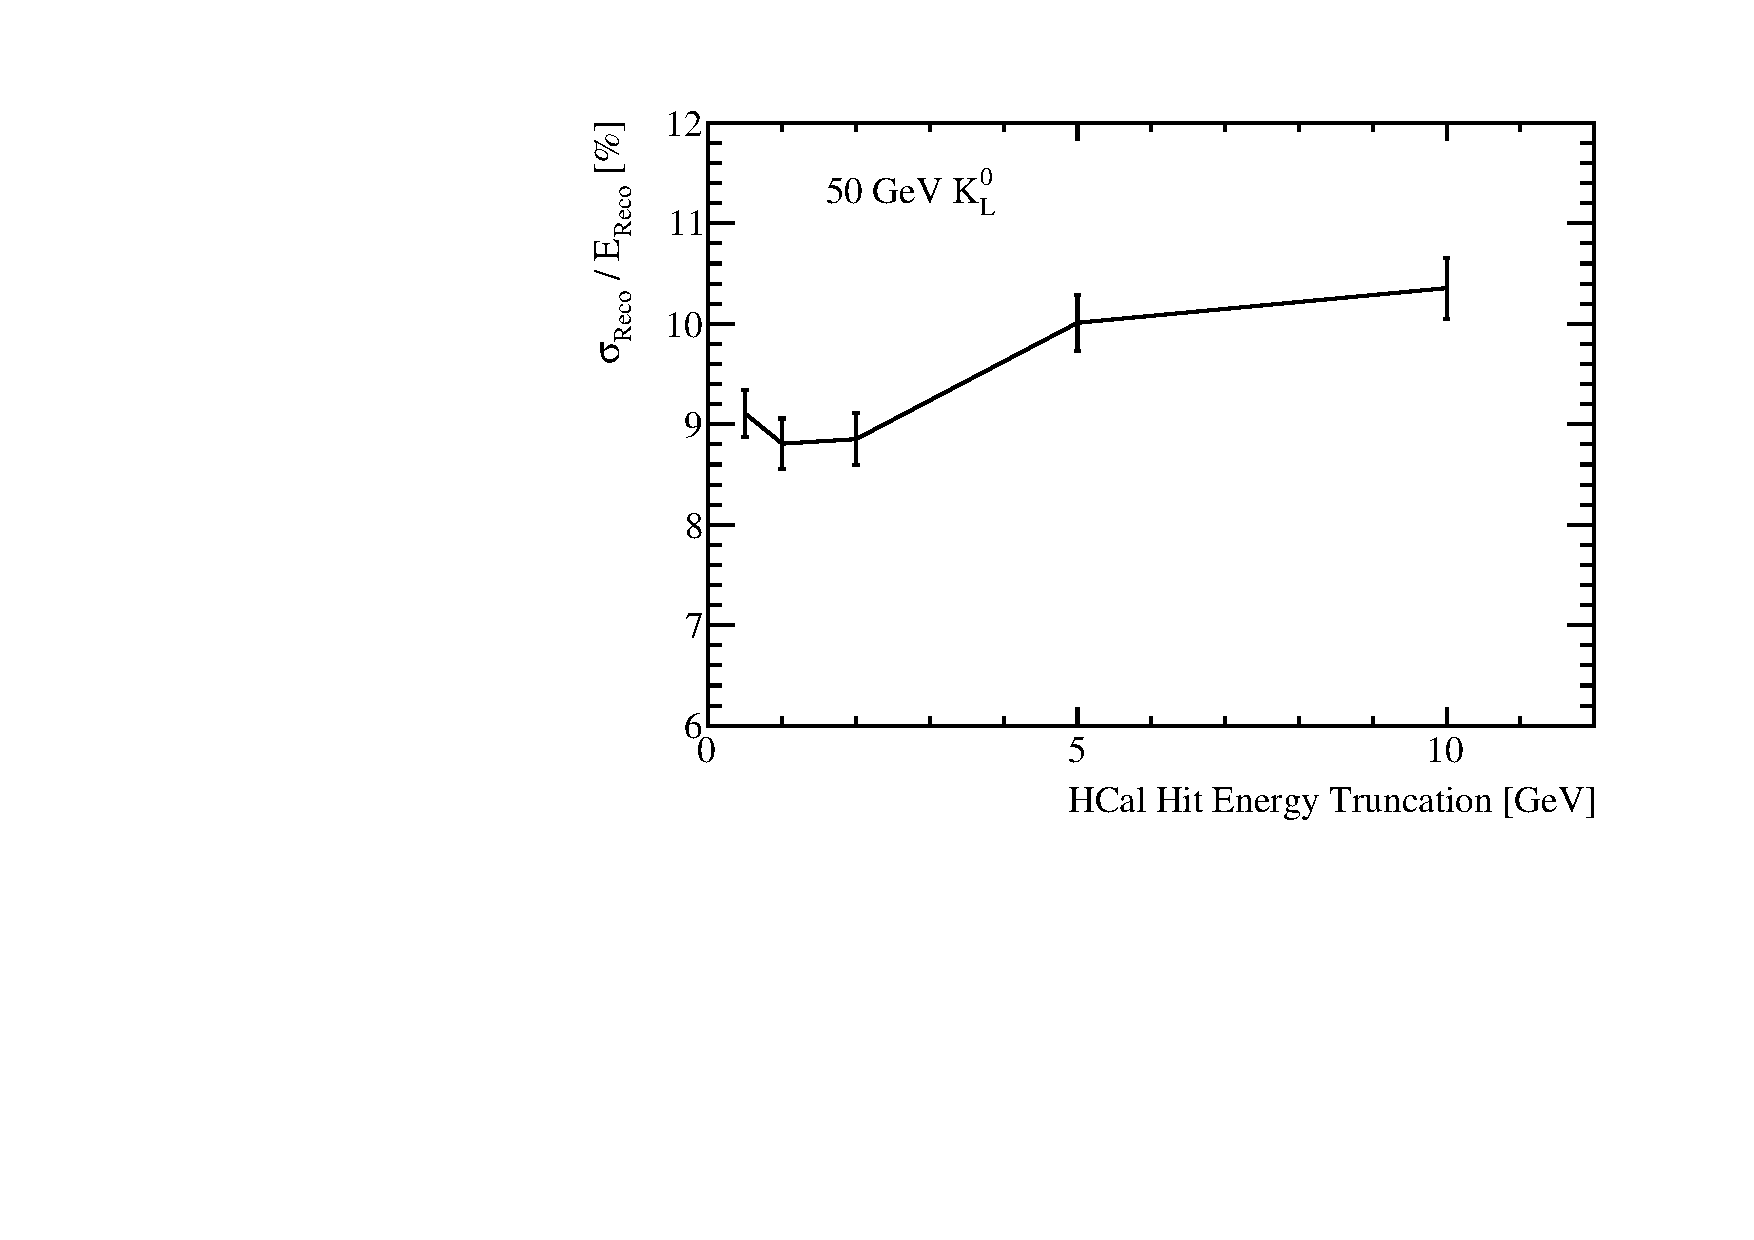
\includegraphics[width=0.5\textwidth]{EnergyEstimators/Plots/CellTruncation/ER_vs_Kaon0LCellTrunc_50GeVKaon0L.pdf}}
\subfloat[]{\label{fig:ercelltruncphotons}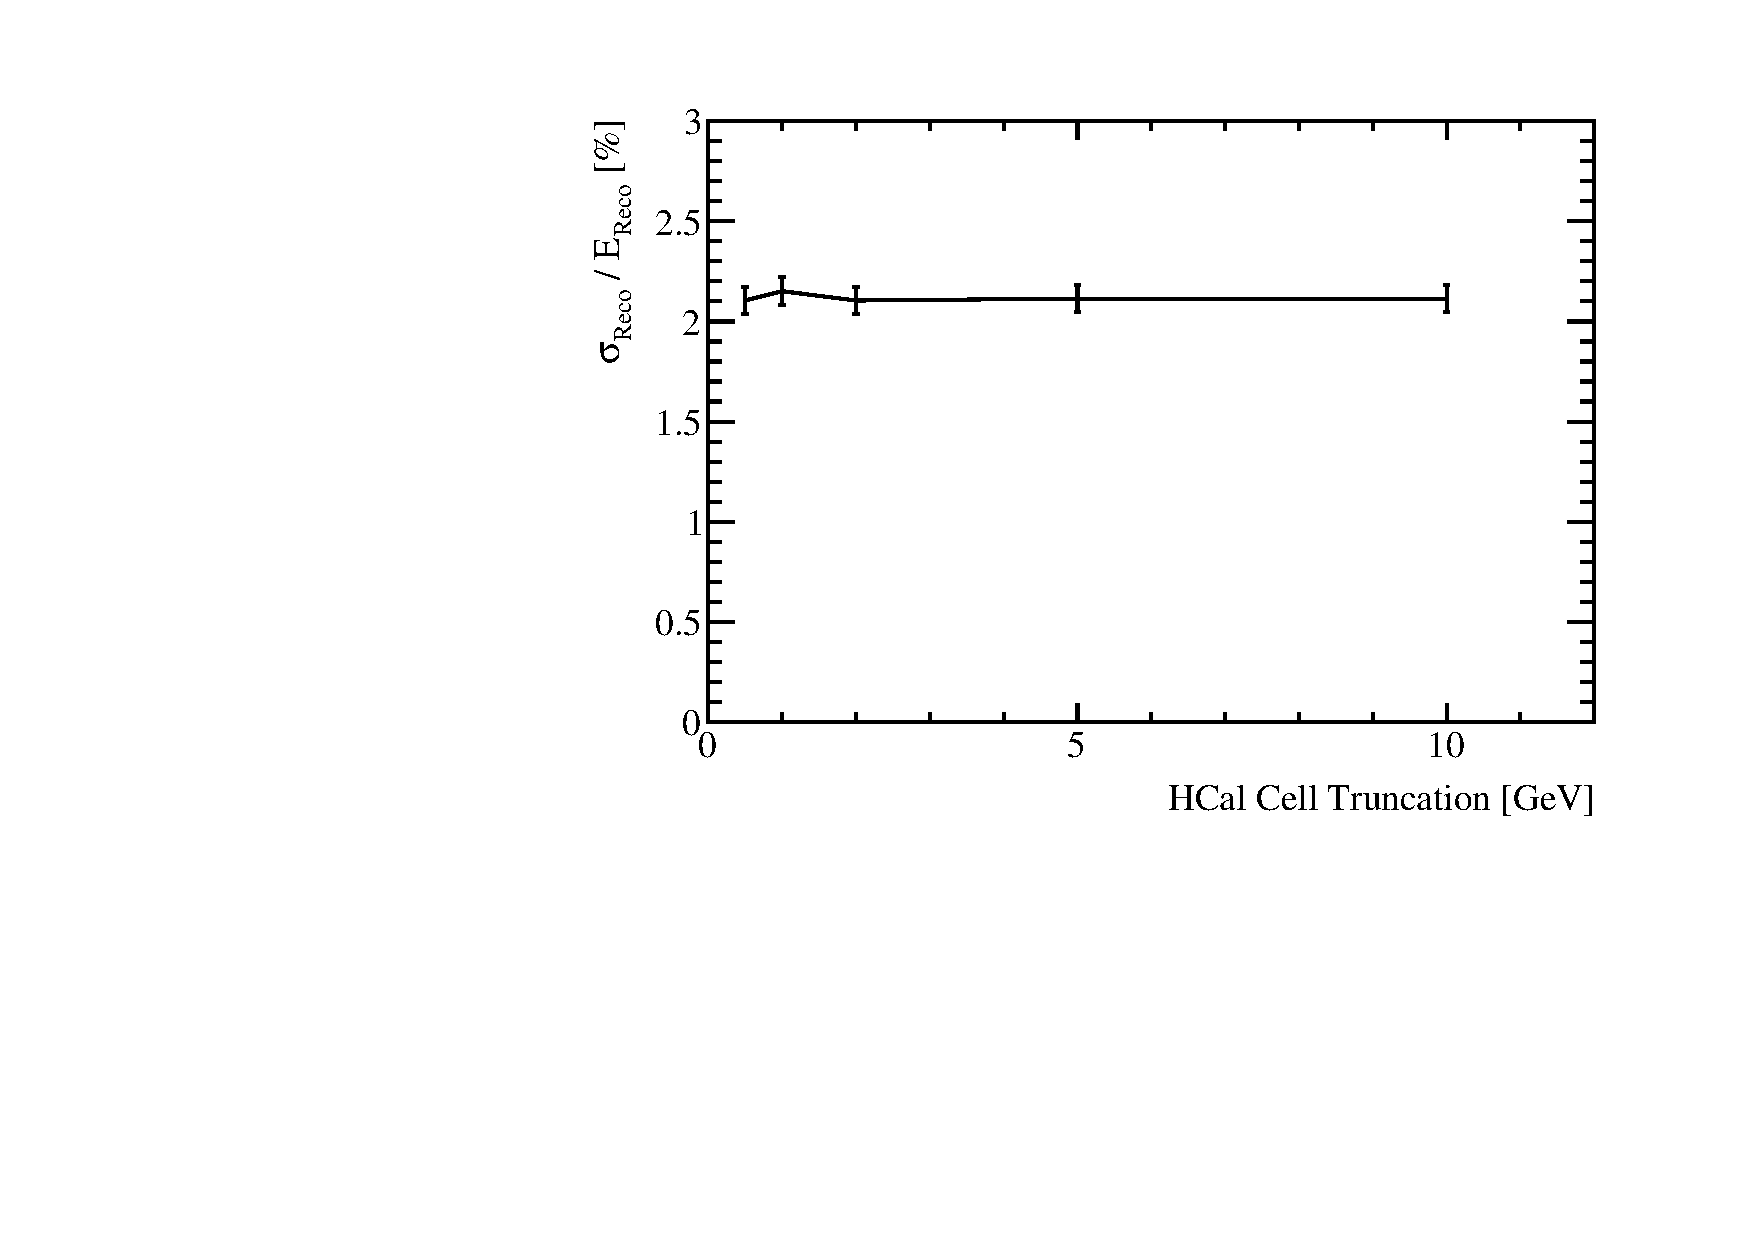
\includegraphics[width=0.5\textwidth]{EnergyEstimators/Plots/CellTruncation/ER_vs_PhotonCellTrunc_100GeVPhoton.pdf}}
\caption[The energy resolution as a function of HCal cell truncation for \protect\subref{fig:ercelltrunckaons} 50 GeV $K^{0}_{L}$ events and \protect\subref{fig:ercelltruncphotons} 100 GeV $\gamma$ events using the nominal ILD detector model.]{The energy resolution as a function of HCal cell truncation for \protect\subref{fig:ercelltrunckaons} 50 GeV $K^{0}_{L}$ events and \protect\subref{fig:ercelltruncphotons} 100 GeV $\gamma$ events using the nominal ILD detector model.}
\label{fig:ercelltrunc}
\end{figure}

%========================================================================================

\subsubsection{Results: Jet Energy Resolution}

The improved energy resolution for careful choice of truncation can be seen in the jet energy resolution.  Figure \ref{fig:jercelltrunc} shows the jet energy resolution as a function of the jet energy for various values of the HCal hit energy truncation.  The trends in this plot are complex as the optimal cell truncation varies with the jet energy.  At low energies a 0.5~GeV truncation gives the best performance, however, when the jet energies reach $\approx$ 180~GeV a 1-2~GeV truncation gives the best performance.  This is to be expected based on the Landau fluctuations.  The Landau distribution, governing the energy deposition for hadronic showers, is essentially a Gaussian with a high energy tail and as the jet energy increases, the mean of the Gaussian increases and the definition of hit energies falling in the high energy tail changes.  

\begin{figure}[h!]
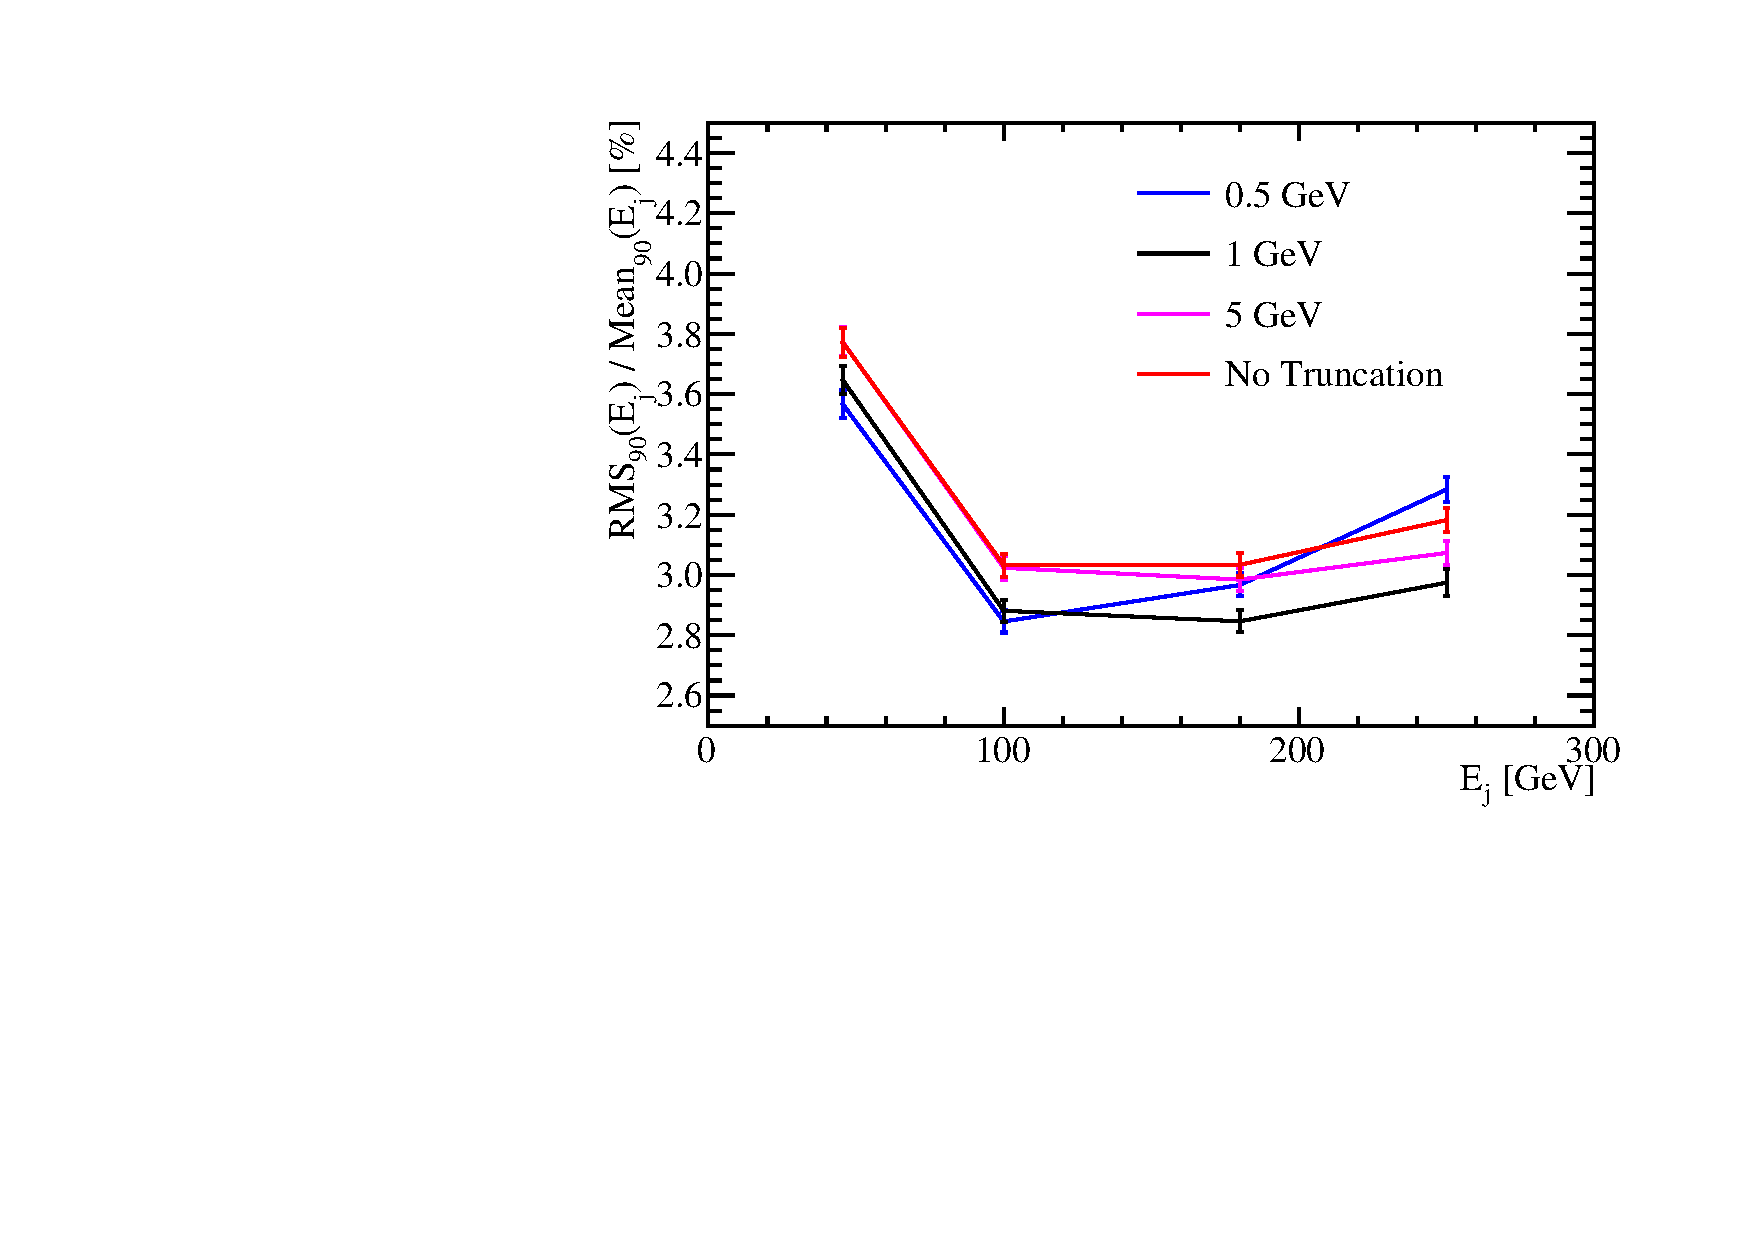
\includegraphics[width=0.5\textwidth]{EnergyEstimators/Plots/CellTruncation/JER_vs_JetEnergy_HCalCellTruncation.pdf}
\caption[The jet energy resolution as a function of jet energy for various hadronic cell truncations.  The results shown use the nominal ILD detector model.]{The jet energy resolution as a function of jet energy for various hadronic cell truncations.  The results shown use the nominal ILD detector model.}
\label{fig:jercelltrunc}
\end{figure}

While it is challenging to determine the optimal performance for a given detector model it is clear that applying an appropriate truncation produces significant improvement in detector performance.  Therefore, for the optimisation studies presented in chapter \ref{chap:detopt} this form of novel energy estimator is applied.  The optimal truncation for each detector model considered in that study was determined by performing the reconstruction using range of HCal hit energy truncations and quoting the optimal performance.  The HCal hit energy truncations considered in the optimisation study were 0.5, 0.75, 1, 1.5, 2, 5, 10, and $10^{6}$ GeV (semi-infinite).  For the HCal cell size study the truncation used for the 10, 20, 30, 40, 50 and 100~mm cell size detector was 0.5, 0.75, 1, 1.5, 2 and 5~GeV respectively, for the tungsten HCal options the truncation used was 5~GeV and for all other options the truncation used was 1~GeV.  This optimisation has a significant impact on detector optimisation, which can be seen by comparing the jet energy resolutions obtained when using the optimised cell truncation and a fixed 1~GeV truncation, shown in figure \ref{fig:jerhcalcellopt}.  Without this optimisation of hit energy truncation the significance of the HCal cell size is overinflated and could lead to a misinformed detector design choice.  

\begin{figure}[h!]
\subfloat[]{\label{fig:jerhcalcelloptgoodtrunc}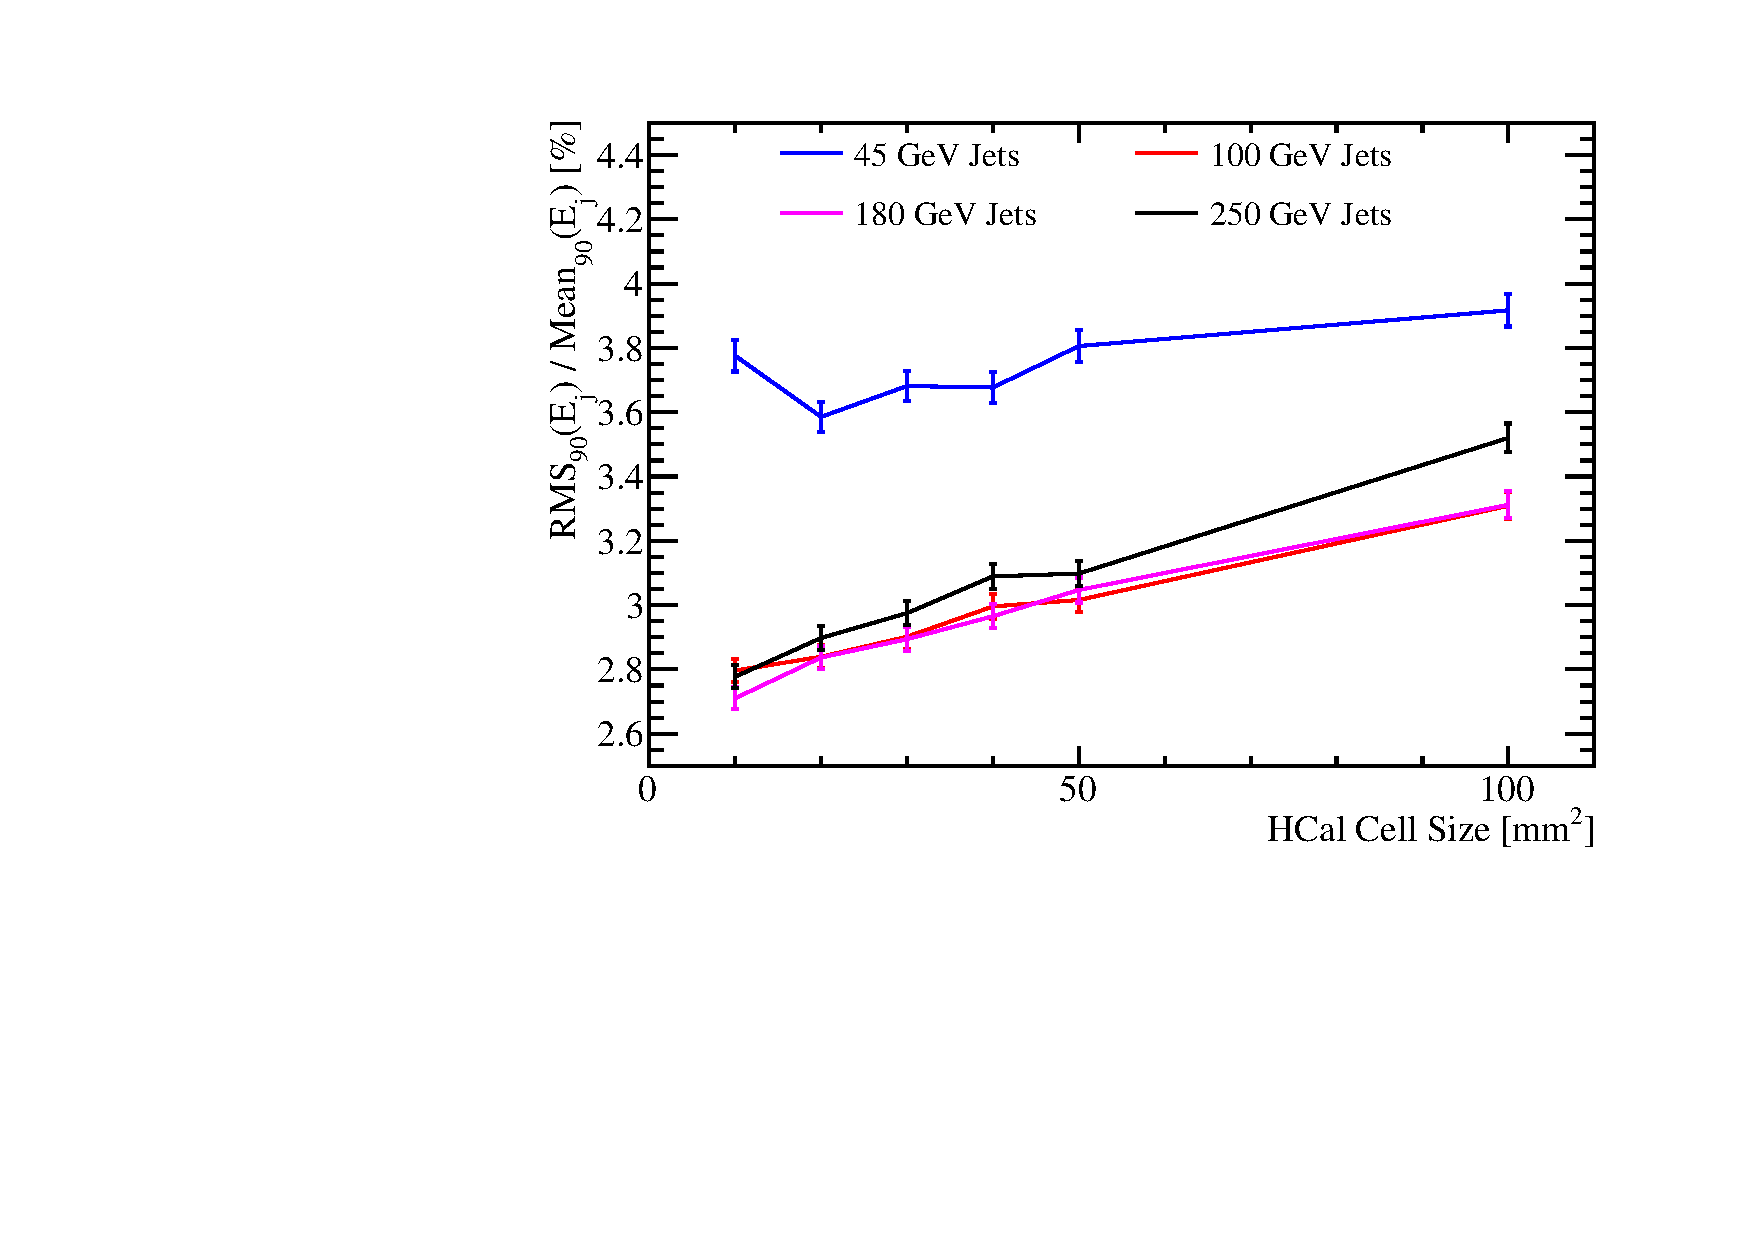
\includegraphics[width=0.5\textwidth]{OptimisationStudies/Plots/JetEnergyResolutions/JER_vs_HCalCellSize.pdf}}
\subfloat[]{\label{fig:jerhcalcelloptbadtrunc}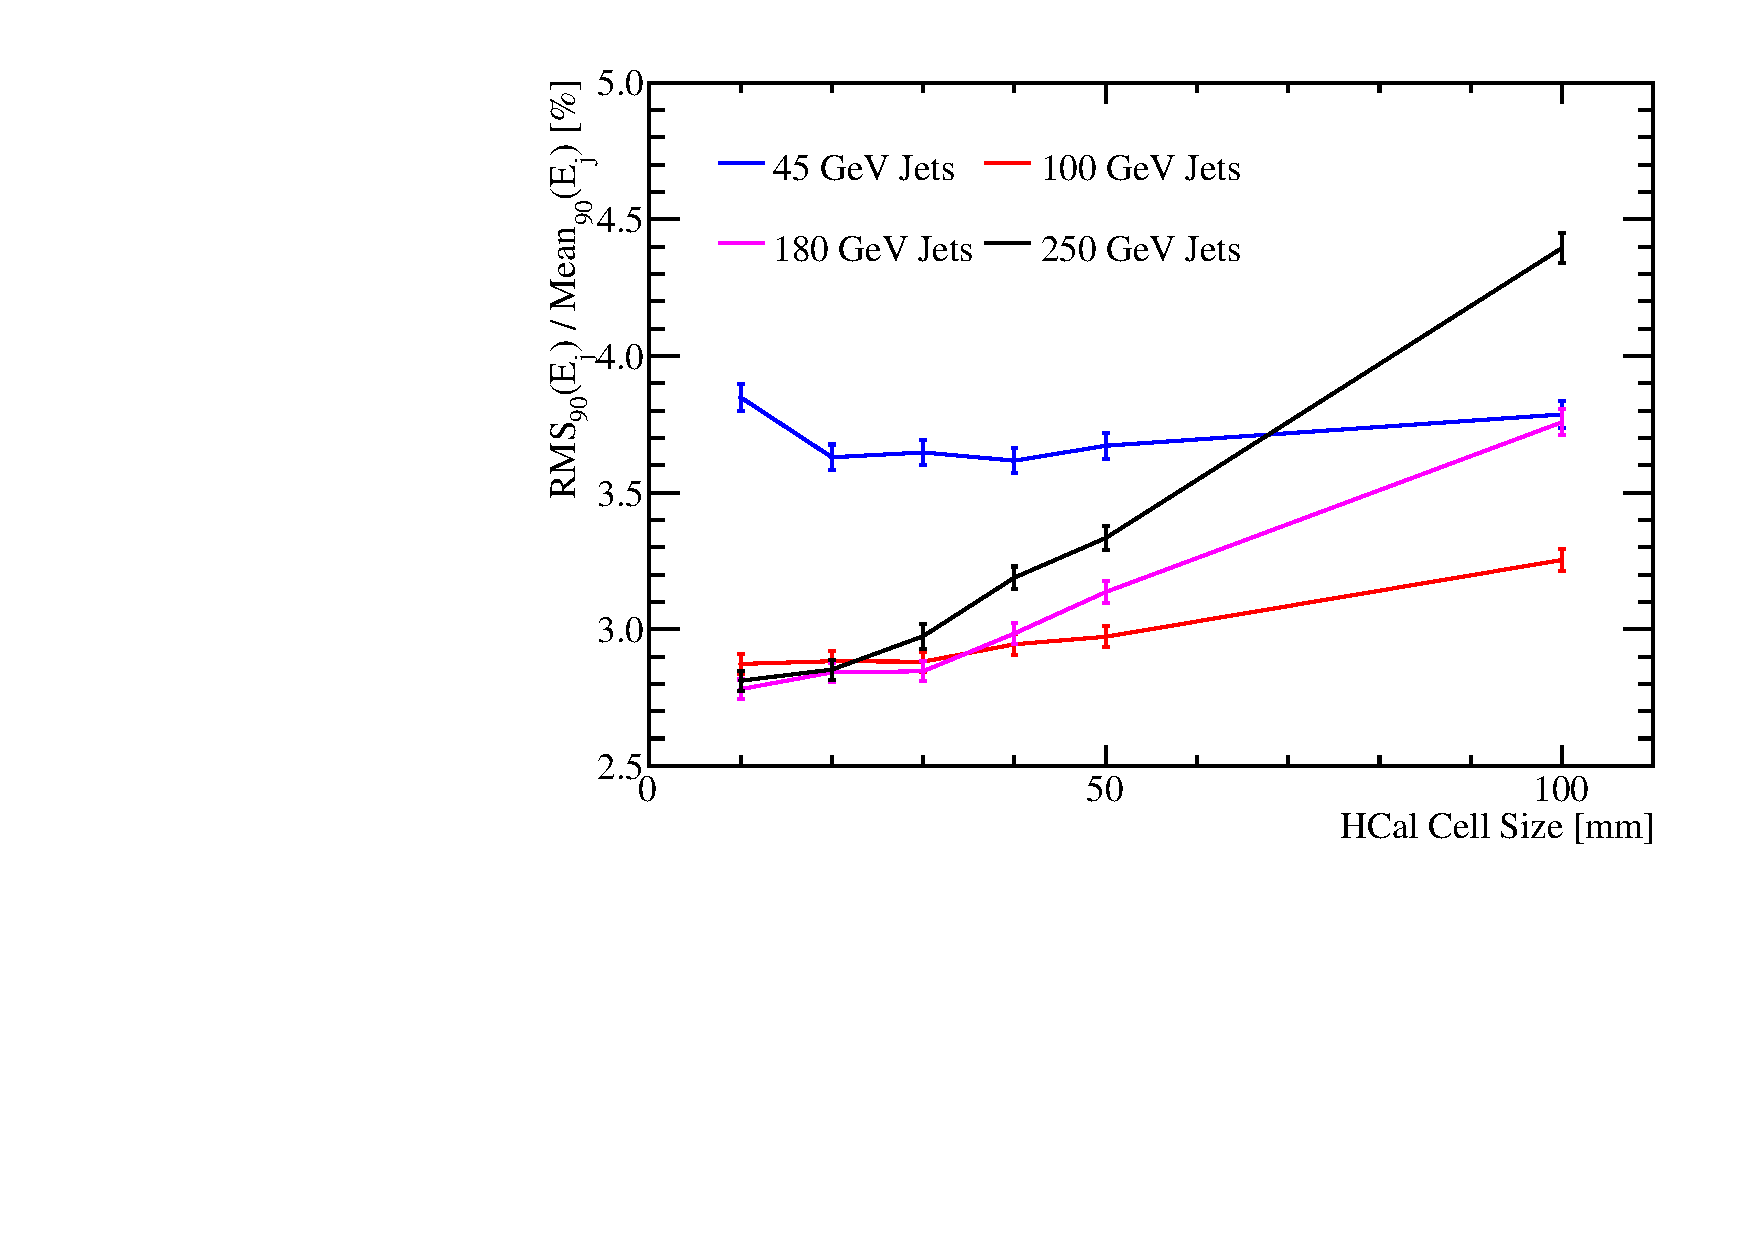
\includegraphics[width=0.5\textwidth]{EnergyEstimators/Plots/CellTruncation/JER_vs_HCalCellSizeBadTruncation.pdf}}
\caption[The jet energy resolution as a function of HCal cell size using a HCal hit energy truncation that is \protect\subref{fig:jerhcalcelloptgoodtrunc} optimised and \protect\subref{fig:jerhcalcelloptbadtrunc} fixed at 1~GeV.]{The jet energy resolution as a function of HCal cell size using a HCal hit energy truncation that is \protect\subref{fig:jerhcalcelloptgoodtrunc} optimised and \protect\subref{fig:jerhcalcelloptbadtrunc} fixed at 1~GeV.}
\label{fig:jerhcalcellopt}
\end{figure}

%========================================================================================

\subsection{Software Compensation}
\label{sec:softcomp}
\subsubsection{Application}
A particle shower produced when a hadron passing through a calorimeter has two components \cite{Wigmans:2000vf}; an electromagnetic shower core, which originates from the production and decay of $\pi^{0}$s and $\eta$s, and a hadronic shower component originating from all other interacting and decaying particles in in the shower.  By identifying each of these components in the reconstruction, it is possible to increase the energy of the hadronic hits to give a compensating response and decrease the energy of spuriously high energy hits that arise from Landau fluctuations.  The challenge of applying this approach is to identify whether a hit is likely to be hadronic or electromagnetic in nature.  This is done based on the energy density of the hit, with high energy densities likely to be part of the electromagnetic core and the low energy densities likely to be part of the satellite hadronic hits of the shower.  An event display showing the energy density of a hadronic shower, where the electromagnetic core can be clearly seen, of a hadronic cluster in a 500 GeV Z$\rightarrow$uds di-jet event can be found in figure \ref{fig:softcompeventdisplay}.  

\begin{figure}[h!]
\subfloat[]{\label{fig:softcompfulleventdisplay}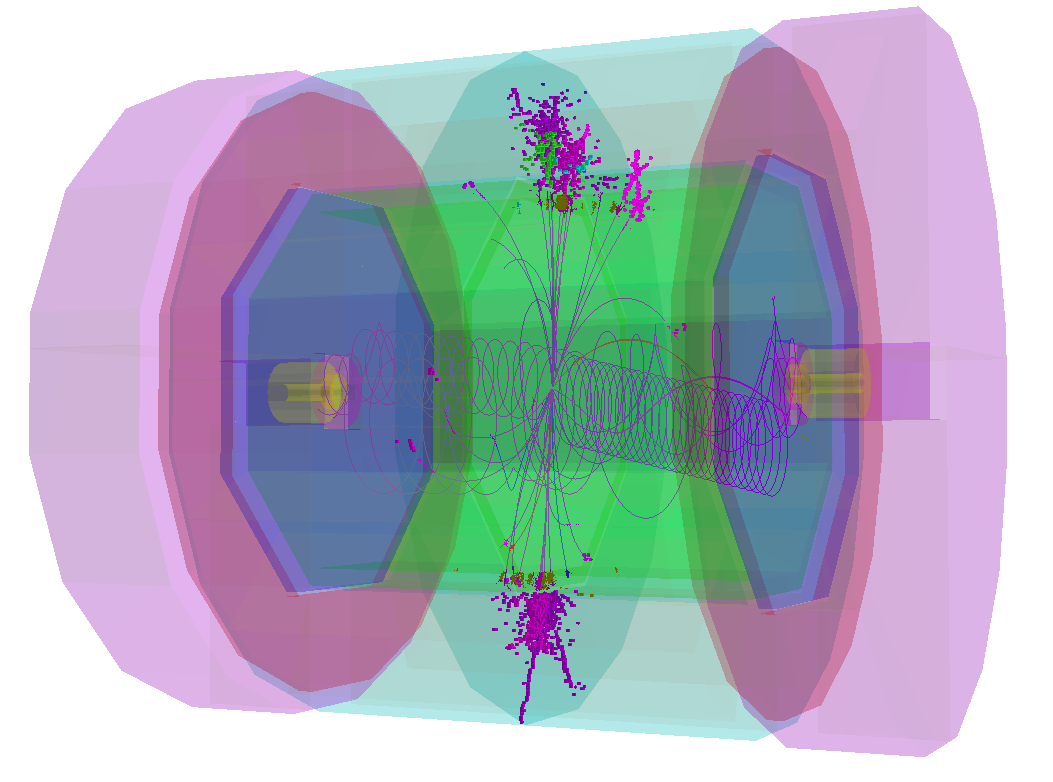
\includegraphics[width=0.5\textwidth]{EnergyEstimators/Plots/SoftComp/VisualDisplay/SoftComp1.png}}
\subfloat[]{\label{fig:softcompclustereventdisplay}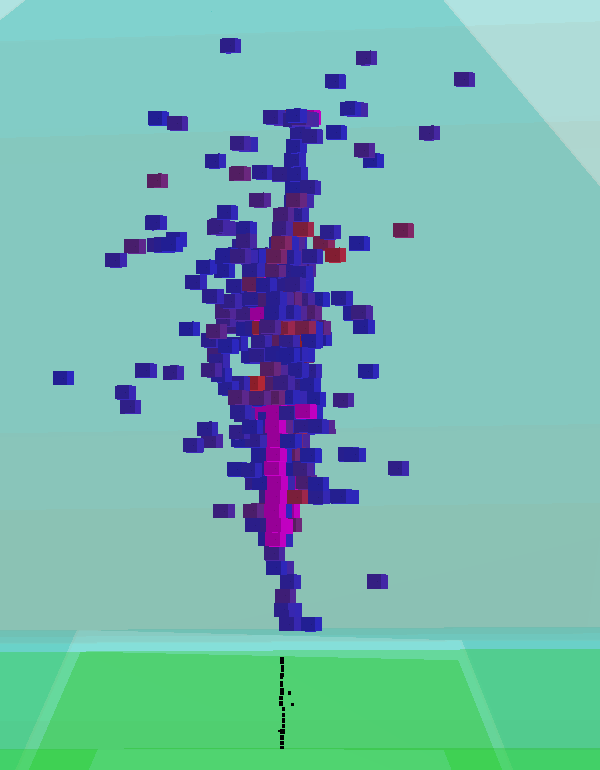
\includegraphics[width=0.3\textwidth]{EnergyEstimators/Plots/SoftComp/VisualDisplay/SoftComp3.png}}
\caption[An event display for a 500 GeV Z$\rightarrow$uds di-jet event reconstructed using the nominal ILD detector.  \protect\subref{fig:softcompfulleventdisplay} The full event environment.  \protect\subref{fig:softcompclustereventdisplay} A single hadronic cluster from the same event where shading indicates the energy density in the HCal.  High energy density cells are coloured red, while lower energy density cells are coloured blue.  All ECal hits are shaded black.  The high energy density electromagnetic core of the selected hadronic cluster is clearly visible.]{An event display for a 500 GeV Z$\rightarrow$uds di-jet event reconstructed using the nominal ILD detector.  \protect\subref{fig:softcompfulleventdisplay} The full event environment.  \protect\subref{fig:softcompclustereventdisplay} A single hadronic cluster from the same event where shading indicates the energy density in the HCal.  High energy density cells are coloured red, while lower energy density cells are coloured blue.  All ECal hits are shaded black.  The high energy density electromagnetic core of the selected hadronic cluster is clearly visible.}
\label{fig:softcompeventdisplay}
\end{figure}

An additional layer of sophistication in this approach is the weights that are applied vary as a function of the uncompensated cluster energy, $E_{\text{Raw}}$, as well as the hit energy density, $\rho^{i}$.  This is to account for the changing energy densities found in hadronic showers as the total shower energy varies.  For example, the fraction of hits in a hadronic shower that are electromagnetic in nature increases as the total energy of the hadronic shower increase \cite{Wigmans:2000vf}.  Therefore, for a high energy hadronic shower fewer hits are purely hadronic in nature and so fewer will require weights that are larger that one.  The highly segmented calorimeters used at the linear collider give excellent resolution on individual particle showers.  This enables precise mapping of the calorimeter hits to different shower components as described above, which allows the linear collider to employ this software compensation technique with greater effectiveness than was possible for previous collider experiments.  

In terms of the $\omega$ weights introduced in equation \ref{equ:compensation}, the weights \cite{Adloff:2012gv} in this technique corresponds to: 
%
\begin{equation}
\omega(E_{\text{Raw}}, \rho) = p_{1}(E_{\text{Raw}}) \times exp(p_{2}(E_{\text{Raw}}) \times \rho) + p_{3}(E_{\text{Raw}}) \\
p_{1} = p_{11} + p_{12} \times E_{\text{Raw}} + p_{13} \times E_{\text{Raw}}^{2} \\
p_{2} = p_{21} + p_{22} \times E_{\text{Raw}} + p_{23} \times E_{\text{Raw}}^{2} \\
p_{3} = \frac{p_{31}}{p_{32} + exp(p_{33} \times E_{\text{Raw}})}\text{ ,}
\label{equ:softcompweight}
\end{equation}
%
\noindent where $p_{ij}$ are trained parameters.  The parameters $p_{ij}$ are determined by performing a $\chi^{2}$ fit of $E_{Cluster}$ using software compensation to the MC energy for samples of $K^{0}_{L}$ ranging from 10 to 100~GeV in steps of 10~GeV.  Using the fitted parameters, $p_{1}$, $p_{2}$ and $p_{3}$ as a function of $E_{\text{Raw}}$ and $\omega(E_{\text{Raw}}, \rho)$ as a function of $\rho$ for various $E_{\text{Raw}}$ are shown in figure \ref{fig:softcompparams} and \ref{fig:softcompweights} respectively.  Figure \ref{fig:softcompweights} shows that the high energy density hits are being reduced in energy to compensate for the effects of Landau fluctuations, while the low energy density hits are being increased in weight to compensate for the invisible energy component found in hadronic showers.  Furthermore, the weights vary as a function of the hadronic shower raw energy to account for the change in fraction of the shower energy appearing in the electromagnetic shower core.  

\begin{figure}[h!]
\subfloat[]{\label{fig:softcompparam1}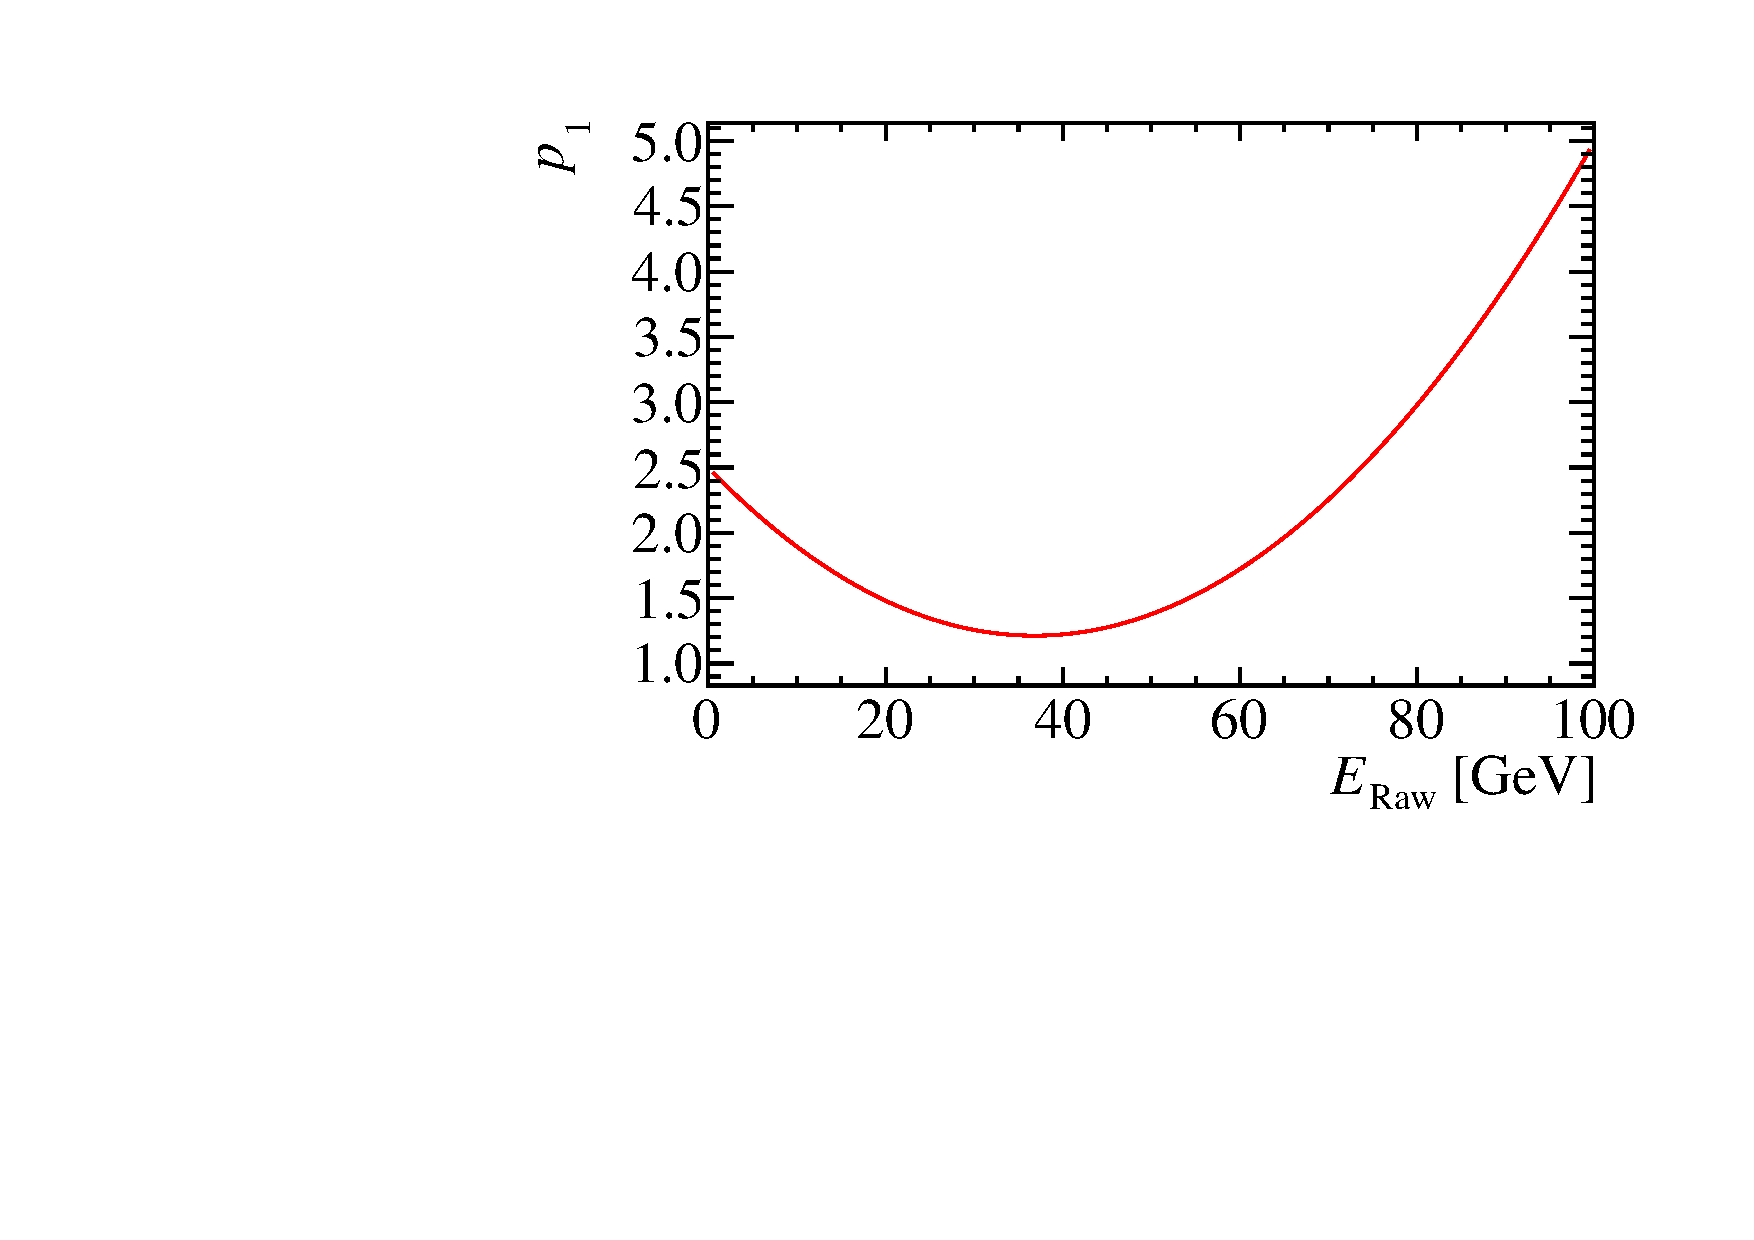
\includegraphics[width=0.33\textwidth]{EnergyEstimators/Plots/SoftComp/Weights/SoftwareCompensationParam1.pdf}}
\subfloat[]{\label{fig:softcompparam2}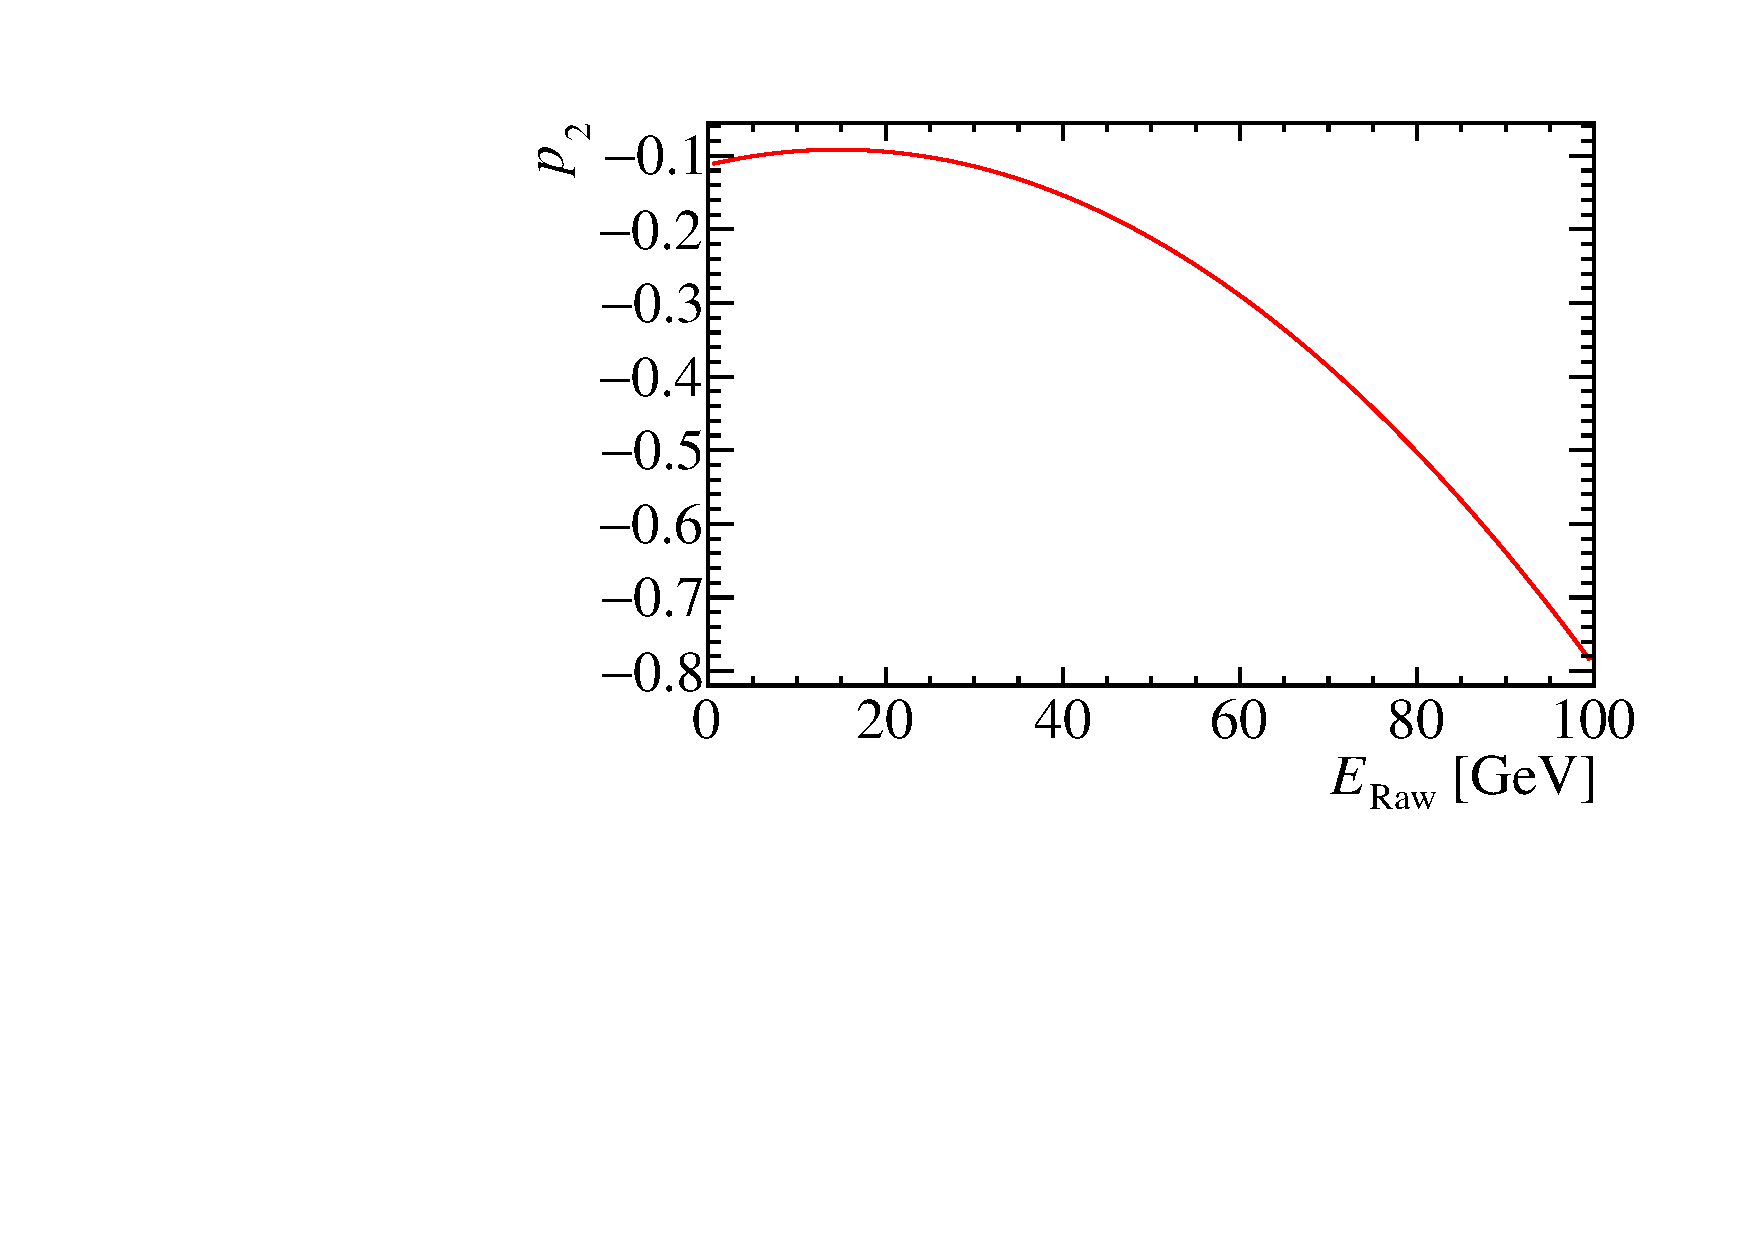
\includegraphics[width=0.33\textwidth]{EnergyEstimators/Plots/SoftComp/Weights/SoftwareCompensationParam2.pdf}}
\subfloat[]{\label{fig:softcompparam3}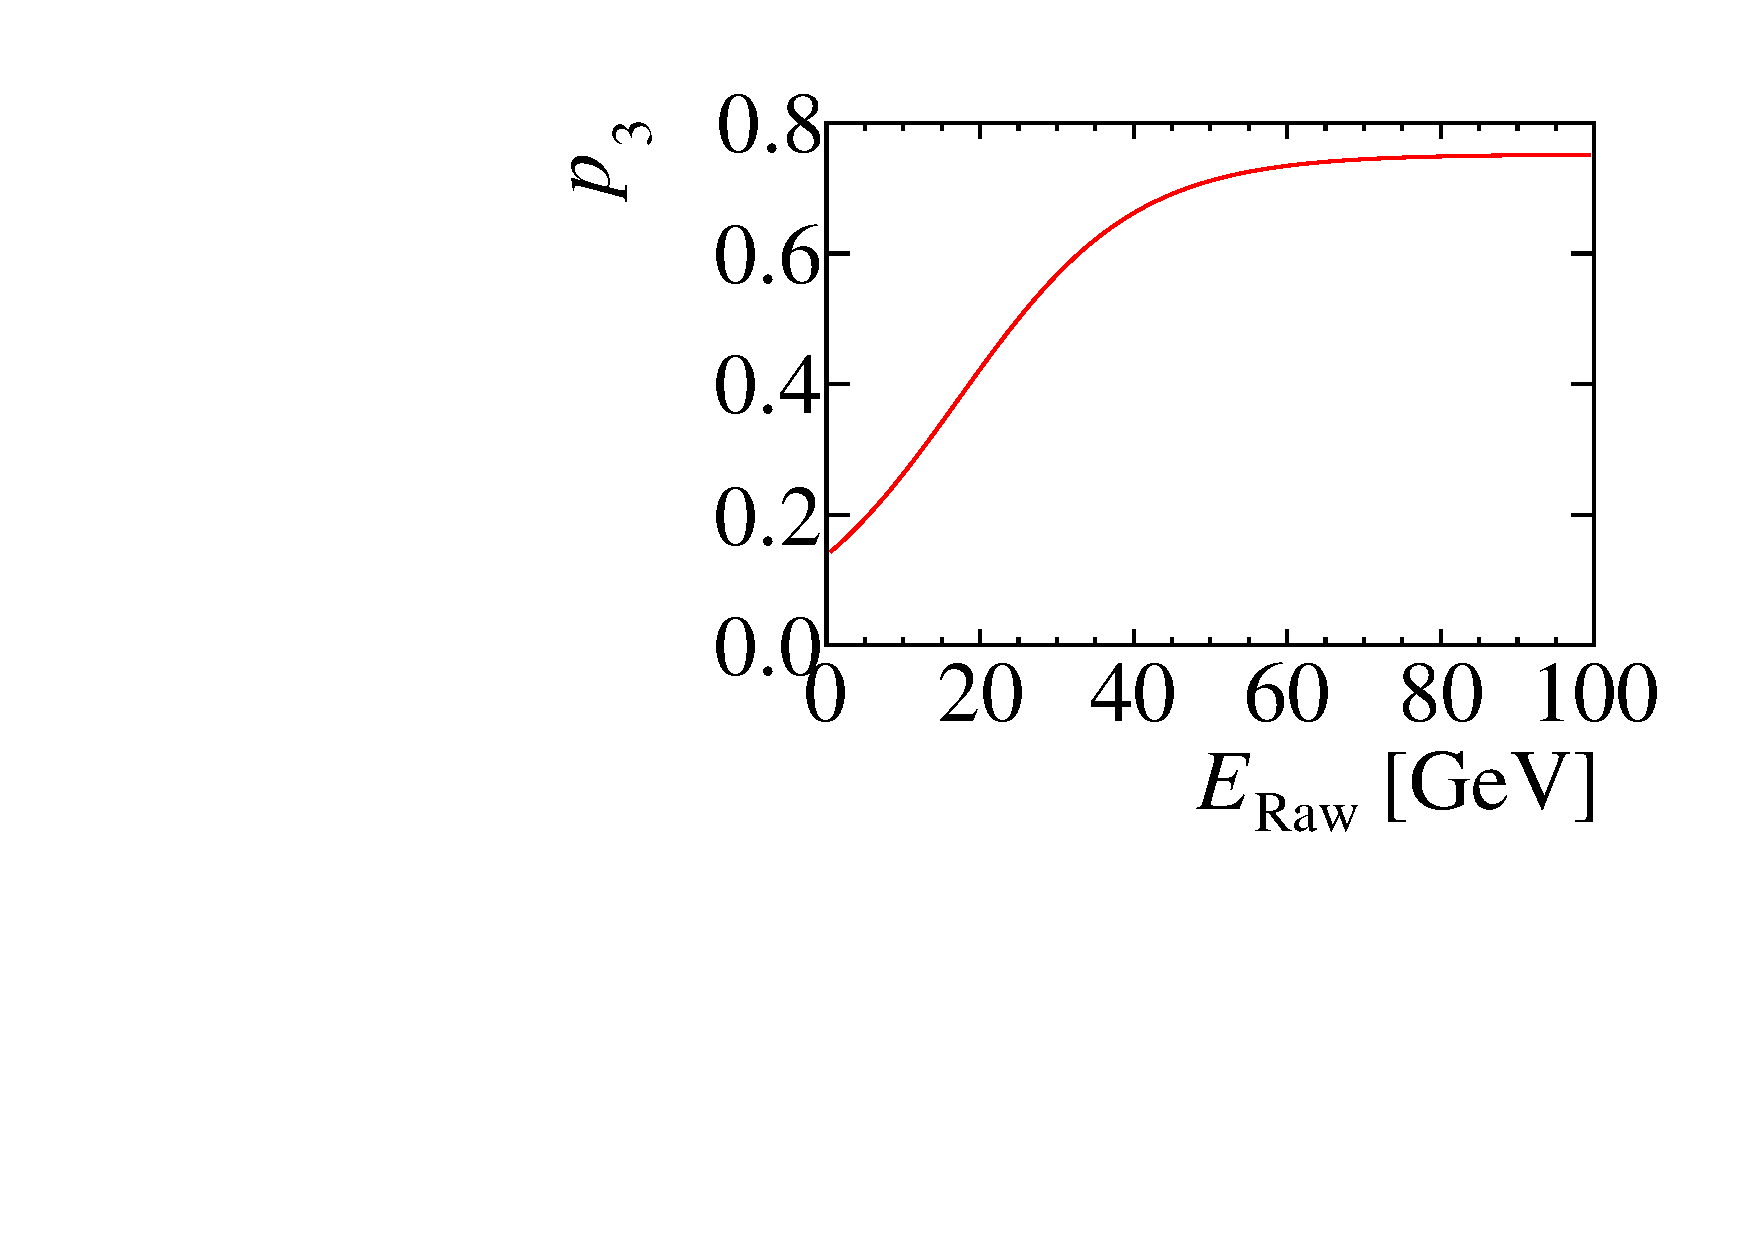
\includegraphics[width=0.33\textwidth]{EnergyEstimators/Plots/SoftComp/Weights/SoftwareCompensationParam3.pdf}}
\caption[Parameters used in software compensation weight determination as a function of $E_{\text{Raw}}$.]{Parameters used in software compensation weight determination as a function of $E_{\text{Raw}}$.}
\label{fig:softcompparams}
\end{figure}

\begin{figure}[h!]
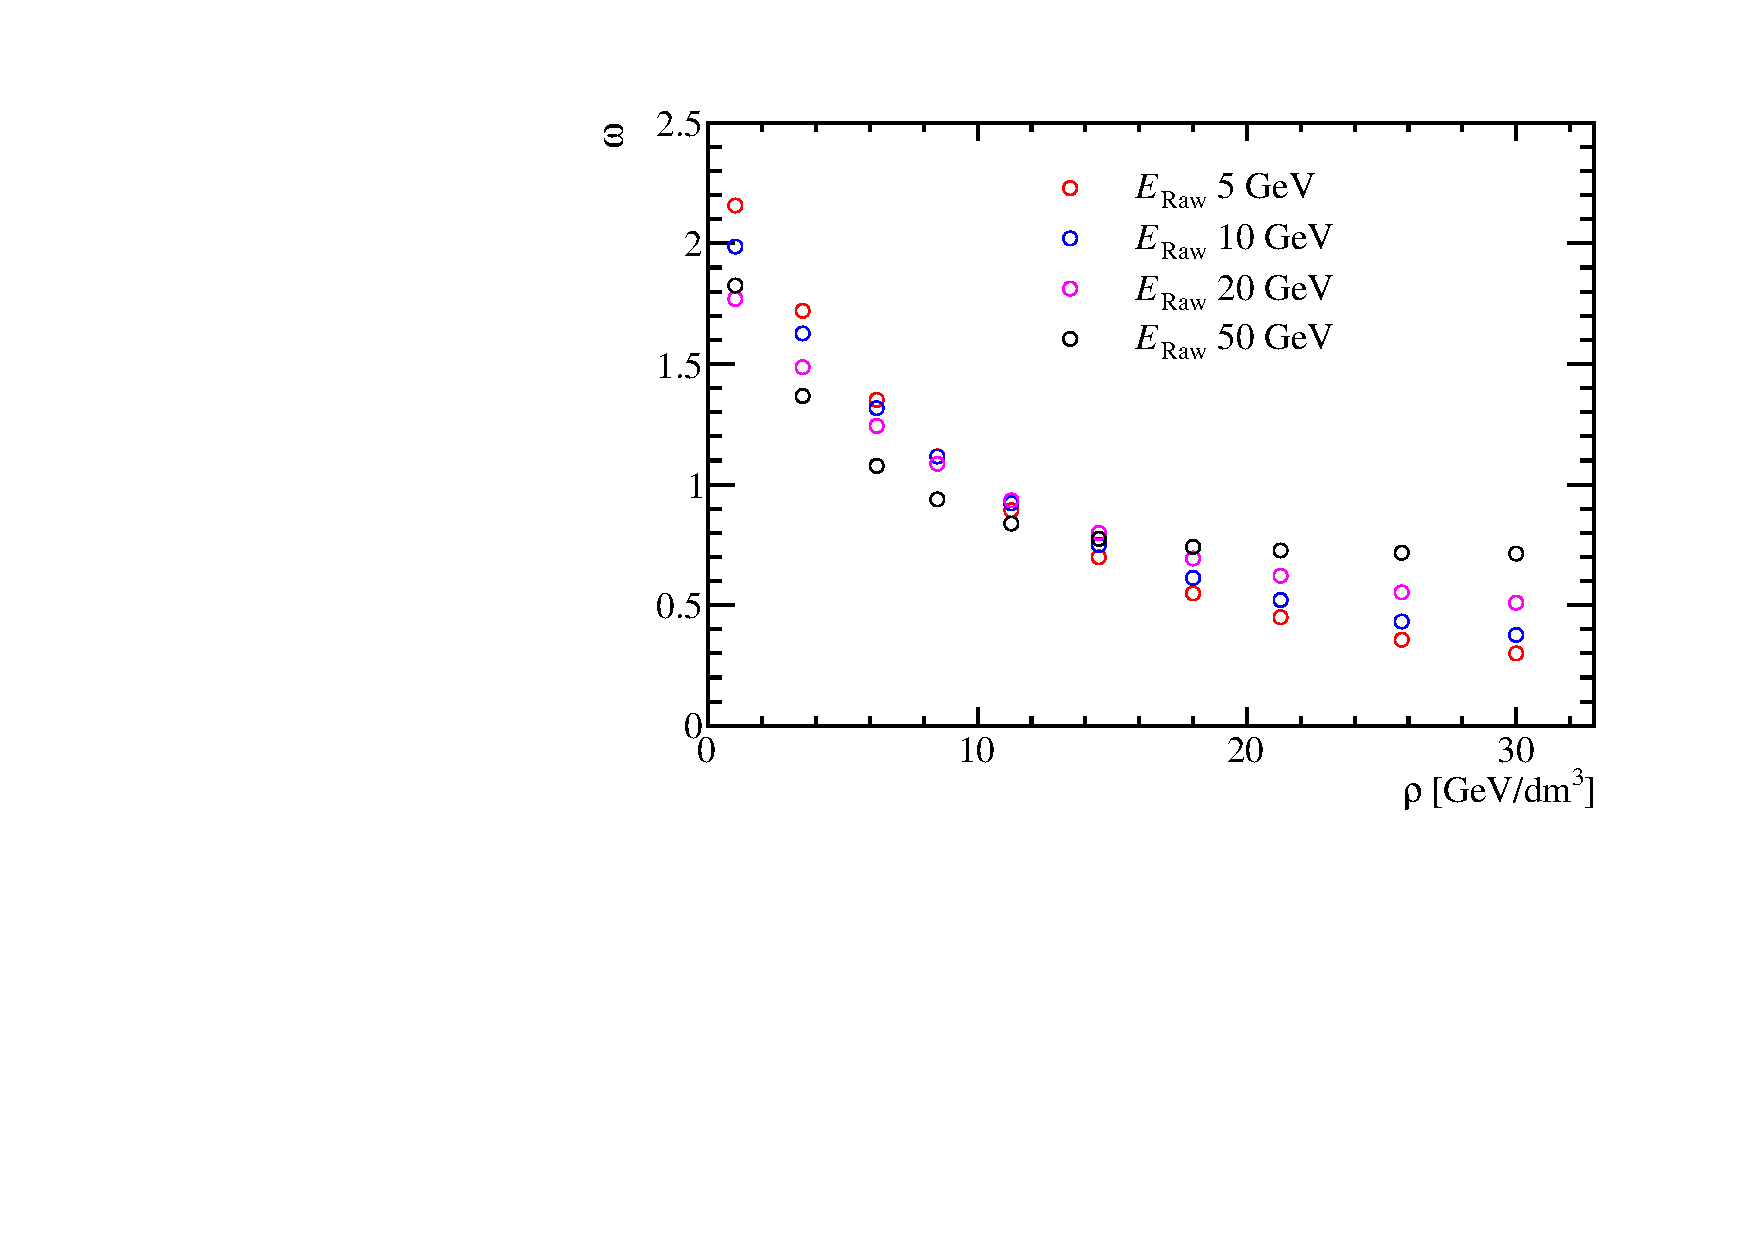
\includegraphics[width=0.5\textwidth]{EnergyEstimators/Plots/SoftComp/Weights/SoftwareCompensationWeights.pdf}
\caption[The software compensation weight applied to a calorimeter hit as a function of calorimeter hit energy density for various cluster energies.]{The software compensation weight applied to a calorimeter hit as a function of calorimeter hit energy density for various cluster energies.}
\label{fig:softcompweights}
\end{figure}

This technique is applied in the PandoraPFA framework in the form of an energy correction function, which means whenever the energy of a cluster of hits is considered by PandoraPFA the software compensated energy is used.  Applying software compensation in this way benefits the detector energy resolution in two ways; firstly the intrinsic energy resolution of the detector improves and secondly the confusion contribution to the energy resolution, from incorrect association of charged particle tracks to calorimeter hit clusters, is reduced.  

As software compensation only modifies the energy of HCal hits there is freedom to apply further energy corrections to the ECal hits.  Application of the Clean Clusters energy correction logic, described in section \ref{sec:legacycorrections}, to the ECal hits alongside software compensation gave further improvements to the jet energy resolution.  Therefore, the application of software compensation within PandoraPFA implicitly involves the application of the Clean Clusters logic to the ECal hits.  

Software compensation is trained using a maximum $K^{0}_{L}$ energy of 100 GeV, therefore, it is only applied to clusters where $E_{\text{Raw}} < 100$ GeV as sensible behaviour outside this range cannot be ensured.  While it would be possible to modify the energy range of the training sample to go to higher energies, hadronic clusters with energy greater than 100 GeV will be rare for the use case considered here.  This is the case as the ILD detector was designed for use at the ILC, which has a maximum running energy of 500 GeV.  

%========================================================================================

\subsubsection{Context: Legacy Energy Corrections}
\label{sec:legacycorrections}
Before examining the impact of software compensation on detector performance is it necessary to address the 'legacy' energy corrections that are used as default in PandoraPFA.  The three energy correction that were in use prior to the development of software compensation are:

\begin{itemize}
\item \textbf{HCal cell truncation}, the details of which can be found in section \ref{sec:hcalcelltruncation}.
\item \textbf{Clean Clusters}.  This algorithm checks to see whether the energy measured within a calorimeter hit is anomalously high.  Anomalously high energy cells are defined as cells where the energy contained within the cell is greater than 10\% of the energy of the cluster that the cell has been associated to.  If a cell is deemed to have an anomalously high energy and if this energy is above a threshold (0.5 GeV) the cell energy used by PandoraPFA is modified.  The updated cell energy is taken as the average cell energy in the calorimeter layers immediately before and after the layer containing the high energy cell.    
\item \textbf{Scale Hot Hadrons}.  This algorithm calculates the average number of MIP equivalent particles passing through each calorimeter cell in a cluster.  If this number is larger than a given value, default 15 MIPs per cell, the cluster energy is rescaled to give a lower average number of MIPs per hit, default is 5 MIPs per hit.  
\end{itemize}

Each of these energy corrections help to deal with the effects of spuriously high energy cells the origin of which is described in section \ref{sec:hcalcelltruncation}.  However, the algorithms are simplistic and software compensation is expected to give far better results than these 'legacy' options.  The optimisation studies presented in section \ref{chap:detopt} use all three of these legacy options simultaneously, which was the default behaviour for PandoraPFA when the studies were undertaken.  The new default behaviour in PandoraPFA is to use software compensation.

%========================================================================================

\subsubsection{Results: Energy Resolution}
\label{sec:softcomper}
The energy resolution as a function of the MC energy for single $K^{0}_{L}$ events is shown in figure \ref{fig:ersoftcomp} using various energy correction settings.  When comparing the energy resolution given by software compensation to that obtained using no energy corrections, it can be seen that software compensation offers a gain of $\approx 2 \%$ in energy resolution across the energy range considered.  The uniformity of this improvement is encouraging, indicating software compensation is achieving a compensating calorimeter response across this wide range of energies.  

Comparing the performance of software compensation to the legacy corrections it can be seen that software compensation gives a better energy resolution across almost the entire range of energies considered.  The only exception to this is around $E_{K^{0}_{L}} \approx 50$~GeV where the performance of software compensation and the legacy corrections are comparable.  By removing the cell truncation from the legacy options it is clear that the changes in energy resolution when using the legacy options are being driven by the cell truncation.  This makes the trend in energy resolution observed using the legacy corrections clear as at low $K^{0}_{L}$ energies very few cells are affected by the truncation so the performance is comparable to not using any energy corrections.  At high $K^{0}_{L}$ energies the truncation is too aggressive and removes energy from cells that are not spuriously high leading to a worsening energy resolution.  Between these two extremes, $E_{K^{0}_{L}} \approx 50$~GeV, the truncation works ideally and improvement in energy resolution using the legacy corrections is the largest.  

\begin{figure}[h!]
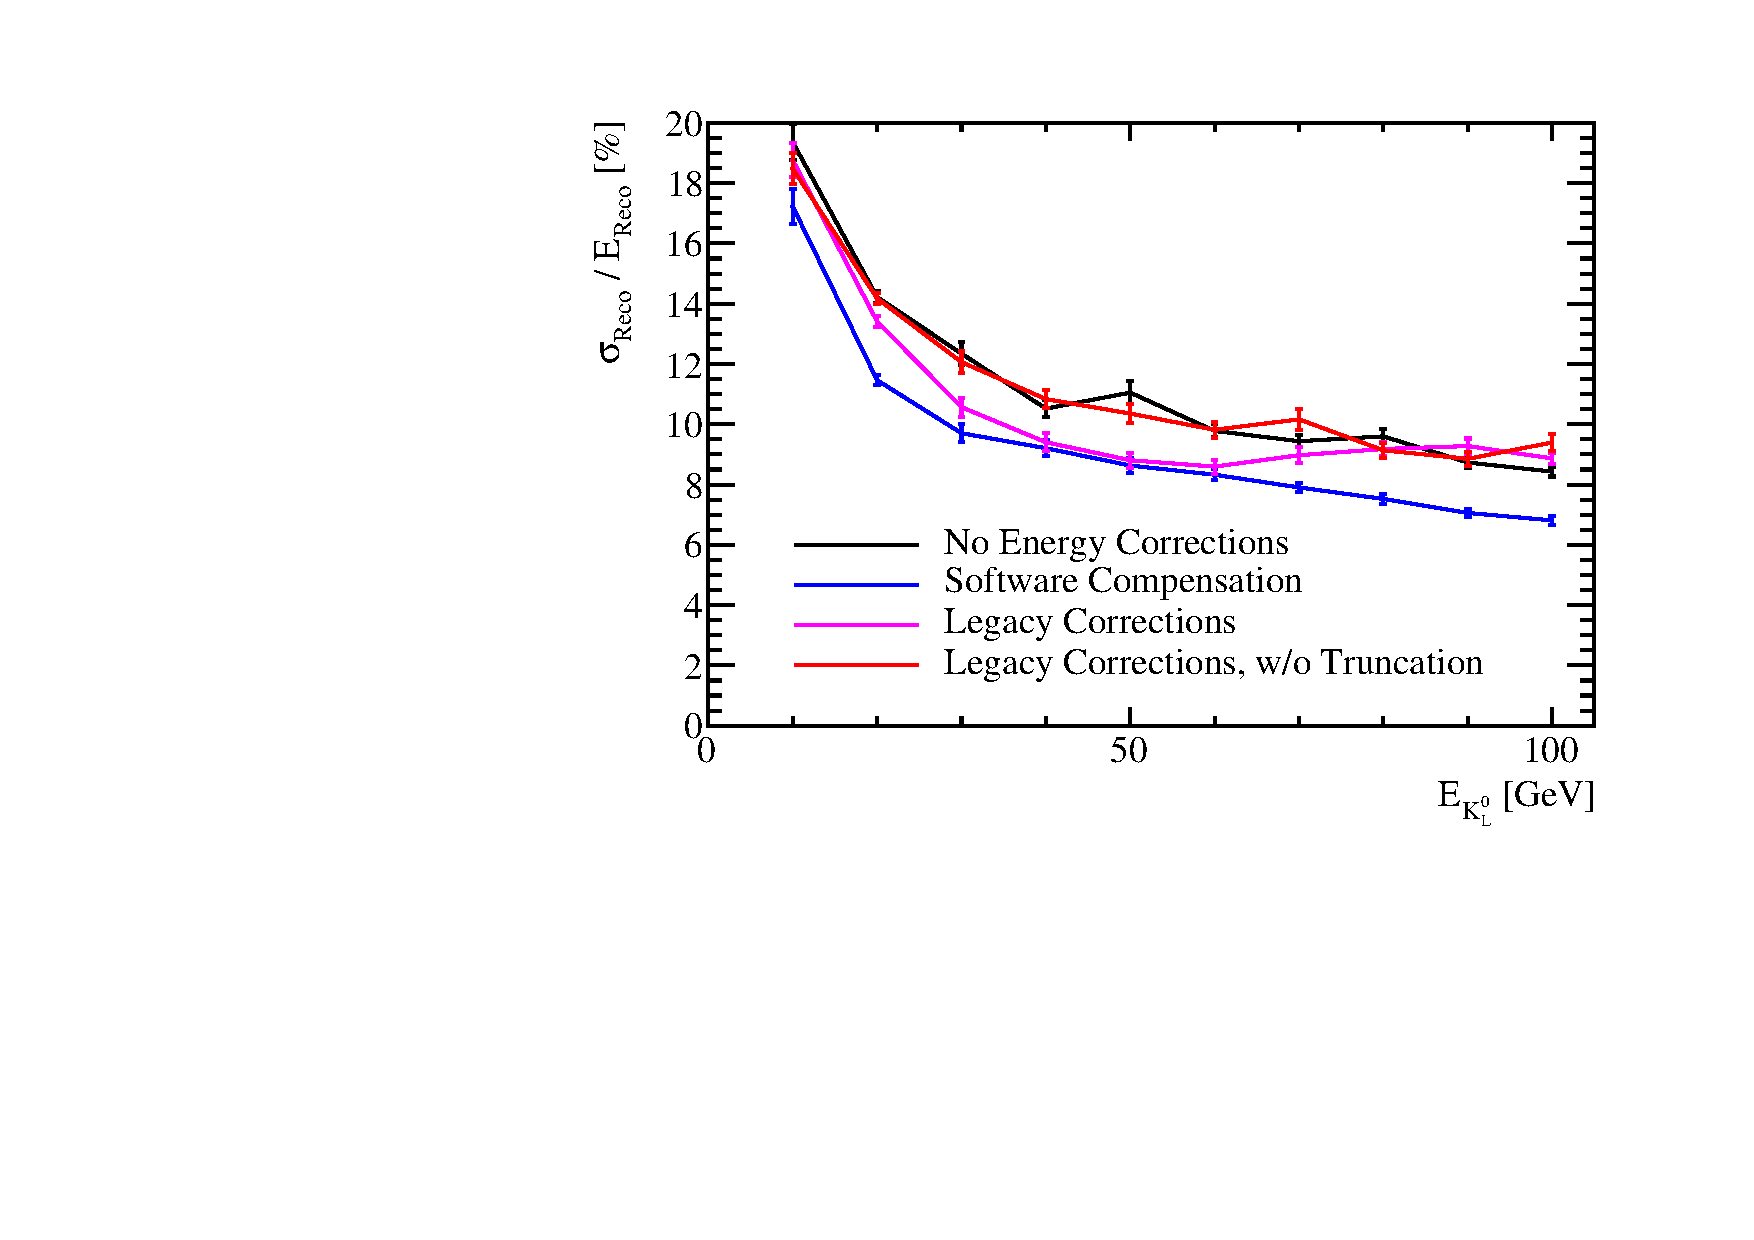
\includegraphics[width=0.5\textwidth]{EnergyEstimators/Plots/SoftComp/EnergyResolution/ER_vs_Kaon0LSoftComp_Kaon0L.pdf}
\caption[The energy resolution as a function of the MC energy for single $K^{0}_{L}$ events using various energy correction settings.  The detector model used was the nominal ILD detector model.]{The energy resolution as a function of the MC energy for single $K^{0}_{L}$ events using various energy correction settings.  The detector model used was the nominal ILD detector model.}
\label{fig:ersoftcomp}
\end{figure}

%========================================================================================

\subsubsection{Results: Jet Energy Resolution}
The improvements in the intrinsic energy resolution of the detector observed when using software compensation will propagate into the reconstruction of jets.  These effects are illustrated by examining the jet energy resolution as a function of jet energy, which is shown in figure \ref{fig:jersoftcomp}.  Again it is clear that software compensation is extremely beneficial to the detector performance.  

\begin{figure}[h!]
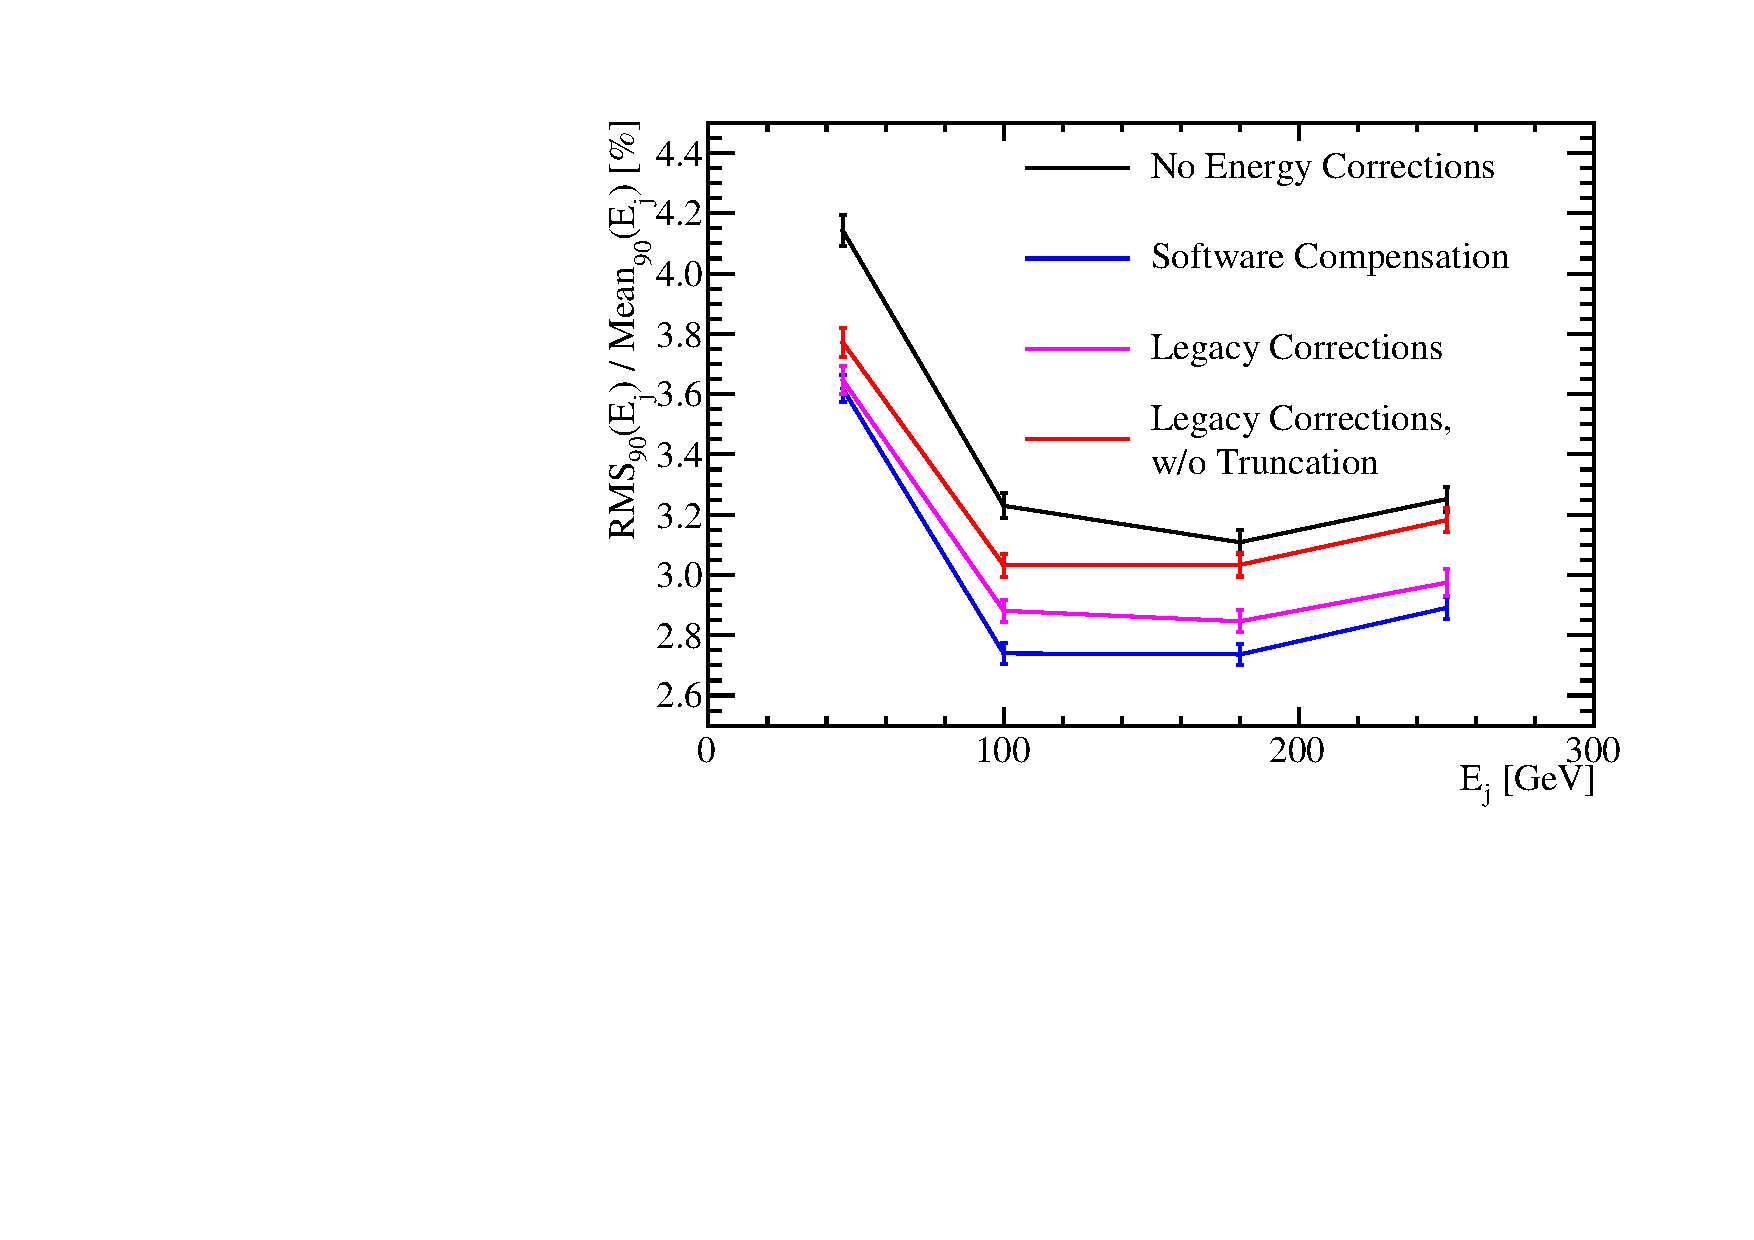
\includegraphics[width=0.5\textwidth]{EnergyEstimators/Plots/SoftComp/JetEnergyResolution/JER_vs_JetEnergy_Default.pdf}
\caption[The jet energy resolution as a function of the jet energy for a variety of different energy correction options.  These results were produced for the nominal ILD detector model.]{The jet energy resolution as a function of the jet energy for a variety of different energy correction options.  These results were produced for the nominal ILD detector model.}
\label{fig:jersoftcomp}
\end{figure}

Software compensation gives a significant reduction in the jet energy resolution in comparison to using no energy corrections.  It also reduces the jet energy resolution in comparison to using the legacy corrections.  

Further light can be shed on these trends by examining the contribution to the jet energy resolutions from the intrinsic energy resolution and the pattern recognition confusion, which are shown in figure \ref{fig:jerbreakdownsoftcomp}.  The intrinsic energy resolution contribution shows that software compensation is significantly better than all other energy corrections options, which is to be expected from the energy resolution studies presented in section \ref{sec:softcomper}.  Unlike the single particle study there is no jet energy for which the cell truncation matches the performance obtained using software compensation.  This is due to the fact that the energy resolution when using the cell truncation is only comparable to the energy resolution using software compensation for a narrow range of hadronic cluster energies.  As the jet contains a broad spectrum of hadronic cluster energies the performance obtained when using the cell truncation will always be worse than when using software compensation.  When comparing the jet energy resolution for the legacy corrections is again apparent that the term driving the jet energy resolution is the cell truncation.

The confusion contribution to the jet energy resolution when using software compensation and the legacy corrections are almost identical.  This indicates that the improvement seen in the jet energy resolution, shown in figure \ref{fig:jersoftcomp}, when using software compensation as opposed to the legacy corrections is being driven by improvements to the intrinsic energy resolution.  At low jet energies the Clean Clusters and Scale Hot Hadrons energy corrections are beneficial at reducing the confusion contribution, while the cell truncation is largely redundant.  For high jet energies jets this trend is reversed.  As the use of the Clean Clusters and Scale Hot Hadrons energy corrections do not alter the intrinsic energy resolution of the detector it is apparently that these energy corrections are purposed to account for failures in the pattern recognition that occur largely at low jet energies.  On the other hand the cell truncation and software compensation techniques aim to improve the energy resolution of the hadronic clusters, which has a knock-on effect of improving the track cluster associations made in the pattern recognition.  These corrections work across all energy ranges, but have a greater impact at high energies.  By extracting the Clean Clusters logic, which is the driving term reducing the confusion contribution to the jet energy resolution at low jet energies, and embedding it within the software compensation energy correction, it is possible to achieve exceptional jet energy resolutions that will extend the physics reach of the linear collider detector.  

\begin{figure}[h!]
\subfloat[]{\label{fig:jerbreakdownsoftcomp1}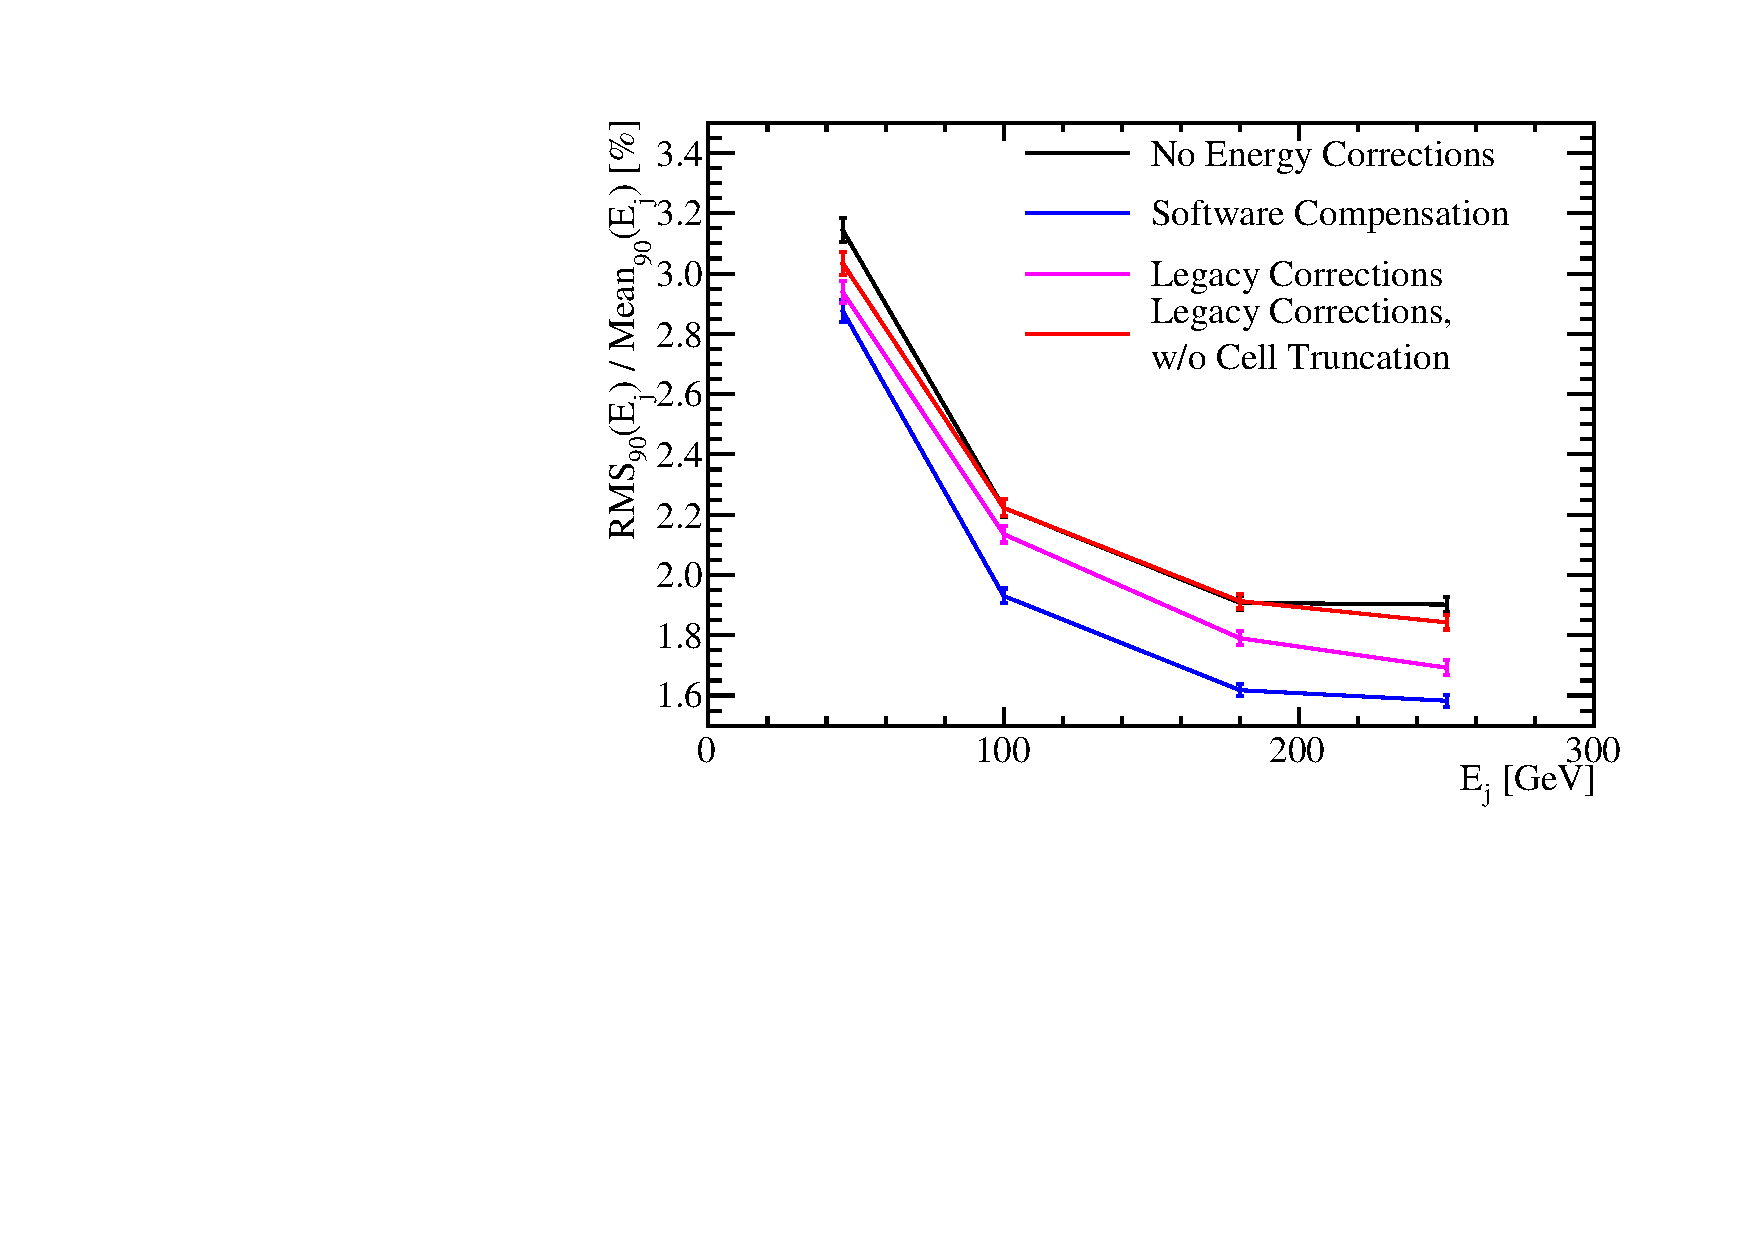
\includegraphics[width=0.5\textwidth]{EnergyEstimators/Plots/SoftComp/JetEnergyResolution/JER_vs_JetEnergy_PerfectPFA.pdf}}
\subfloat[]{\label{fig:jerbreakdownsoftcomp2}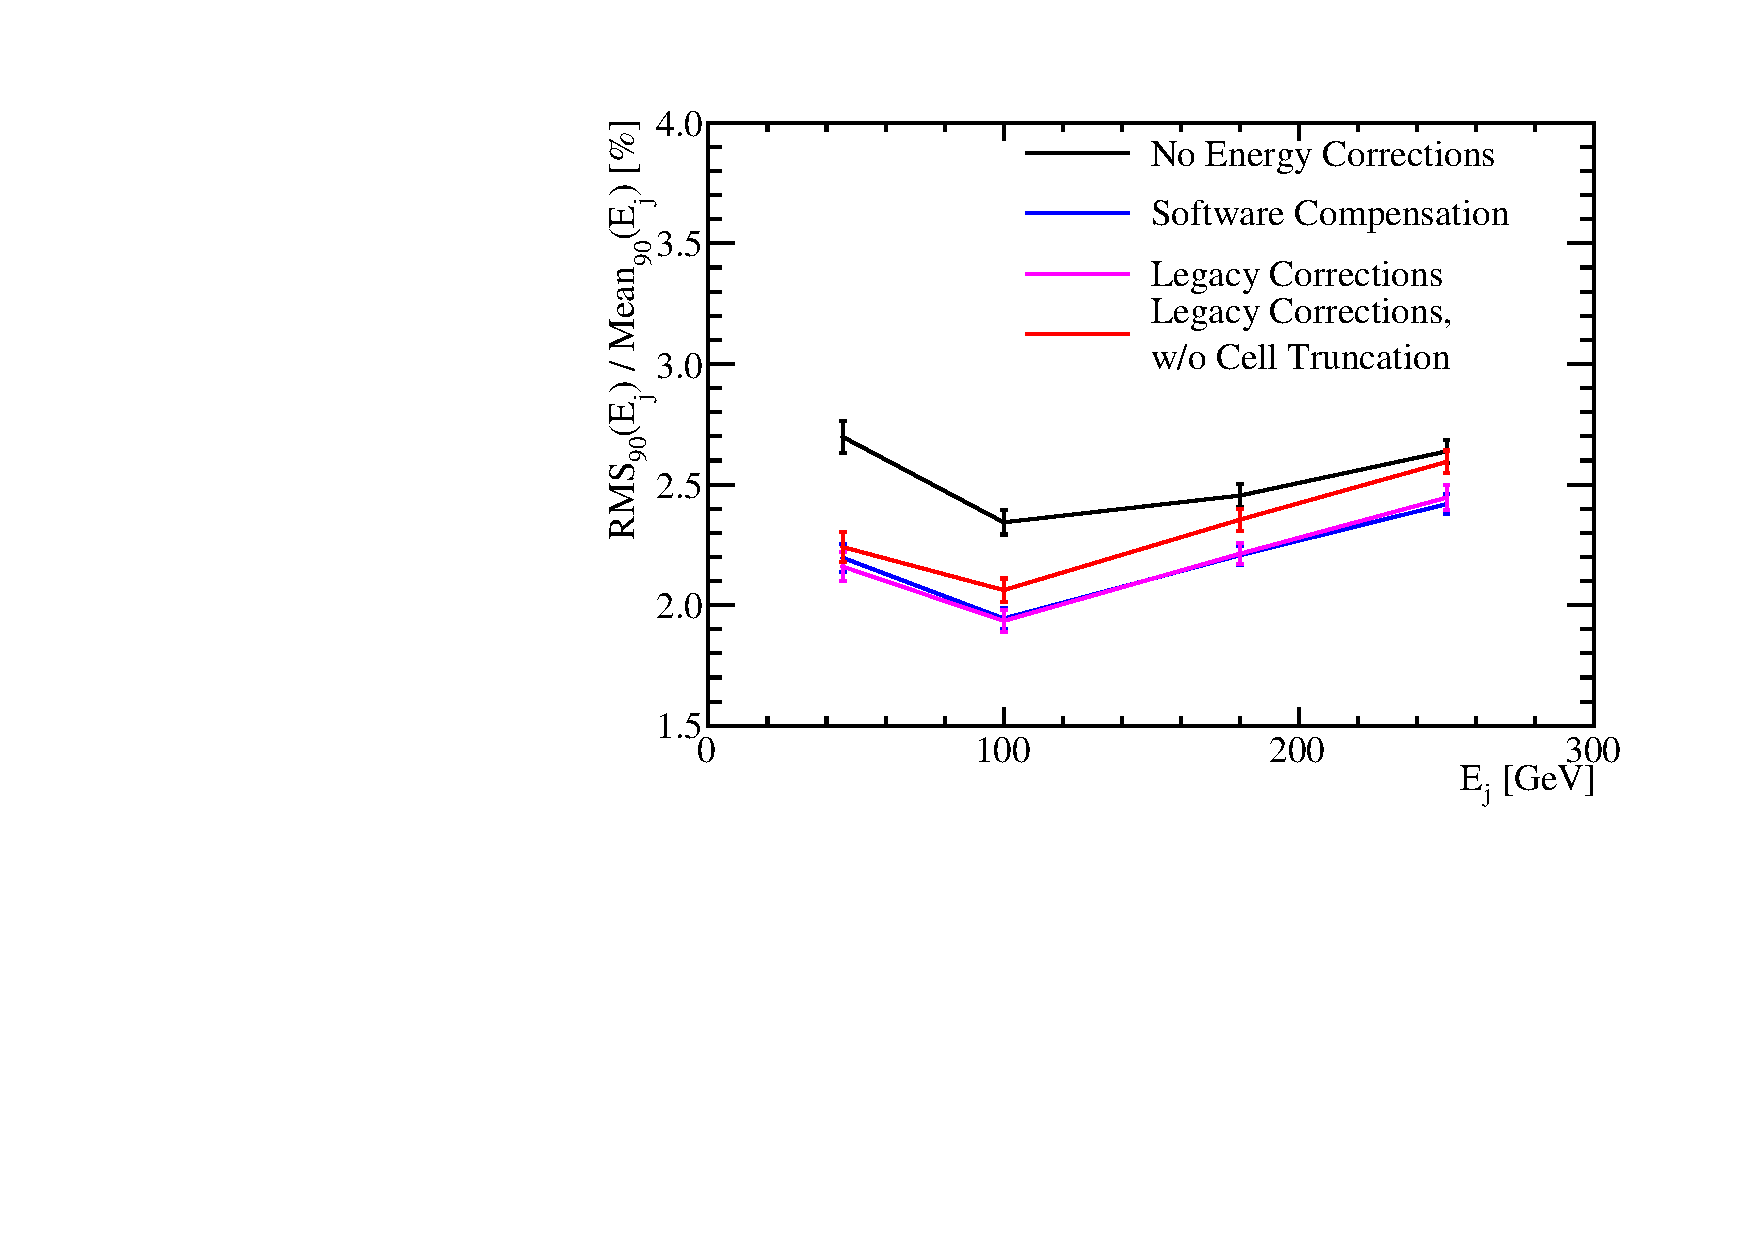
\includegraphics[width=0.5\textwidth]{EnergyEstimators/Plots/SoftComp/JetEnergyResolution/JER_vs_JetEnergy_TotalConfusion.pdf}}
\caption[The contributions to the jet energy resolution as a function of the jet energy for a variety of different energy correction options.  \protect\subref{fig:jerbreakdownsoftcomp1} is the intrinsic energy resolution of the detector and \protect\subref{fig:jerbreakdownsoftcomp2} is the total confusion term.  The quadrature sum of both yields the standard reconstruction performance.  These results were produced for the nominal ILD detector model.]{The contributions to the jet energy resolution as a function of the jet energy for a variety of different energy correction options.  \protect\subref{fig:jerbreakdownsoftcomp1} is the intrinsic energy resolution of the detector and \protect\subref{fig:jerbreakdownsoftcomp2} is the total confusion term.  The quadrature sum of both yields the standard reconstruction performance.  These results were produced for the nominal ILD detector model.}
\label{fig:jerbreakdownsoftcomp}
\end{figure}

%========================================================================================
%========================================================================================

\section{Timing Cuts}
The ILC and CLIC will operate using a trigger-less readout approach whereby the recorded data for each sub-detector is readout between collisions of $\text{e}^{+}$ and $\text{e}^{-}$ bunches.  The train structure for the ILC and CLIC at maximum operating energy is shown in table \ref{table:trainstructure}.  Event selection will proceed through the application of a software trigger.  This involves the identification of hard interactions, prior to full event reconstruction, and only putting data into the event reconstruction if it is measured within a chosen time window about this interaction.  Timing cuts placed on the calorimeter hits are corrected for straight time-of-flight to the IP.  This ensures that the amount of time particle showers have to develop in the calorimeters is independent of their position.  As the size of the time window around the hard interaction changes the amount of time particle showers have to develop varies and this will affect the performance of the detector.  

\begin{table}[h!]
\centering
\begin{tabular}{l r r}
\hline
& ILC 500 GeV & CLIC 3 TeV \\
\hline
Electrons per bunch [$10^{10}$] & 2.0 & 0.37 \\
Bunches per train & 2820 & 312 \\
Train repetition rate [Hz] & 5 & 50 \\
Bunch separation [ns] & 308 & 0.5 \\
\end{tabular}
\caption[The train structure for 500 GeV ILC and 3 TeV CLIC \cite{Behnke:2013lya,Linssen:2012hp}.]{The train structure for 500 GeV ILC and 3 TeV CLIC \cite{Behnke:2013lya,Linssen:2012hp}.}
\label{table:trainstructure}
\end{table}

For all choices of time window considered in this study the calibration procedure was reapplied.  This means that the mean of the reconstructed energy distributions will be invariant to changes in the calorimeter timing window as the calibration procedure compensates for any energy losses incurred by truncating the particle shower development time.  

%========================================================================================

\subsubsection{Results: Energy Resolution}
The energy resolution for 100~GeV $\gamma$ and 50~GeV $K^{0}_{L}$ events as a function of the timing window applied to the calorimeter hits is shown in figure \ref{fig:ertimingcuts} for the nominal ILD detector model .  The timing cut makes little difference to the energy resolution of the $\gamma$ events, however, there is a significant decrease in the energy resolution for the neutral hadrons.  This is to be expected as electromagnetic showers develop far more rapidly than their hadronic counterparts \cite{Wigmans:2000vf}, which can be seen in figure \ref{fig:calohittiming}.  This is expected hadronic showers often involve intermediate states that must decay to continue the propagation of the shower and as these states have non-zero lifetimes they slow the propagation of the shower.  If a narrow calorimeter timing window is used, energy measurements from the hadronic shower will be lost and the energy resolution will degrade, which is what is observed.  

\begin{figure}[h!]
\subfloat[]{\label{fig:ertimingcutsphotons}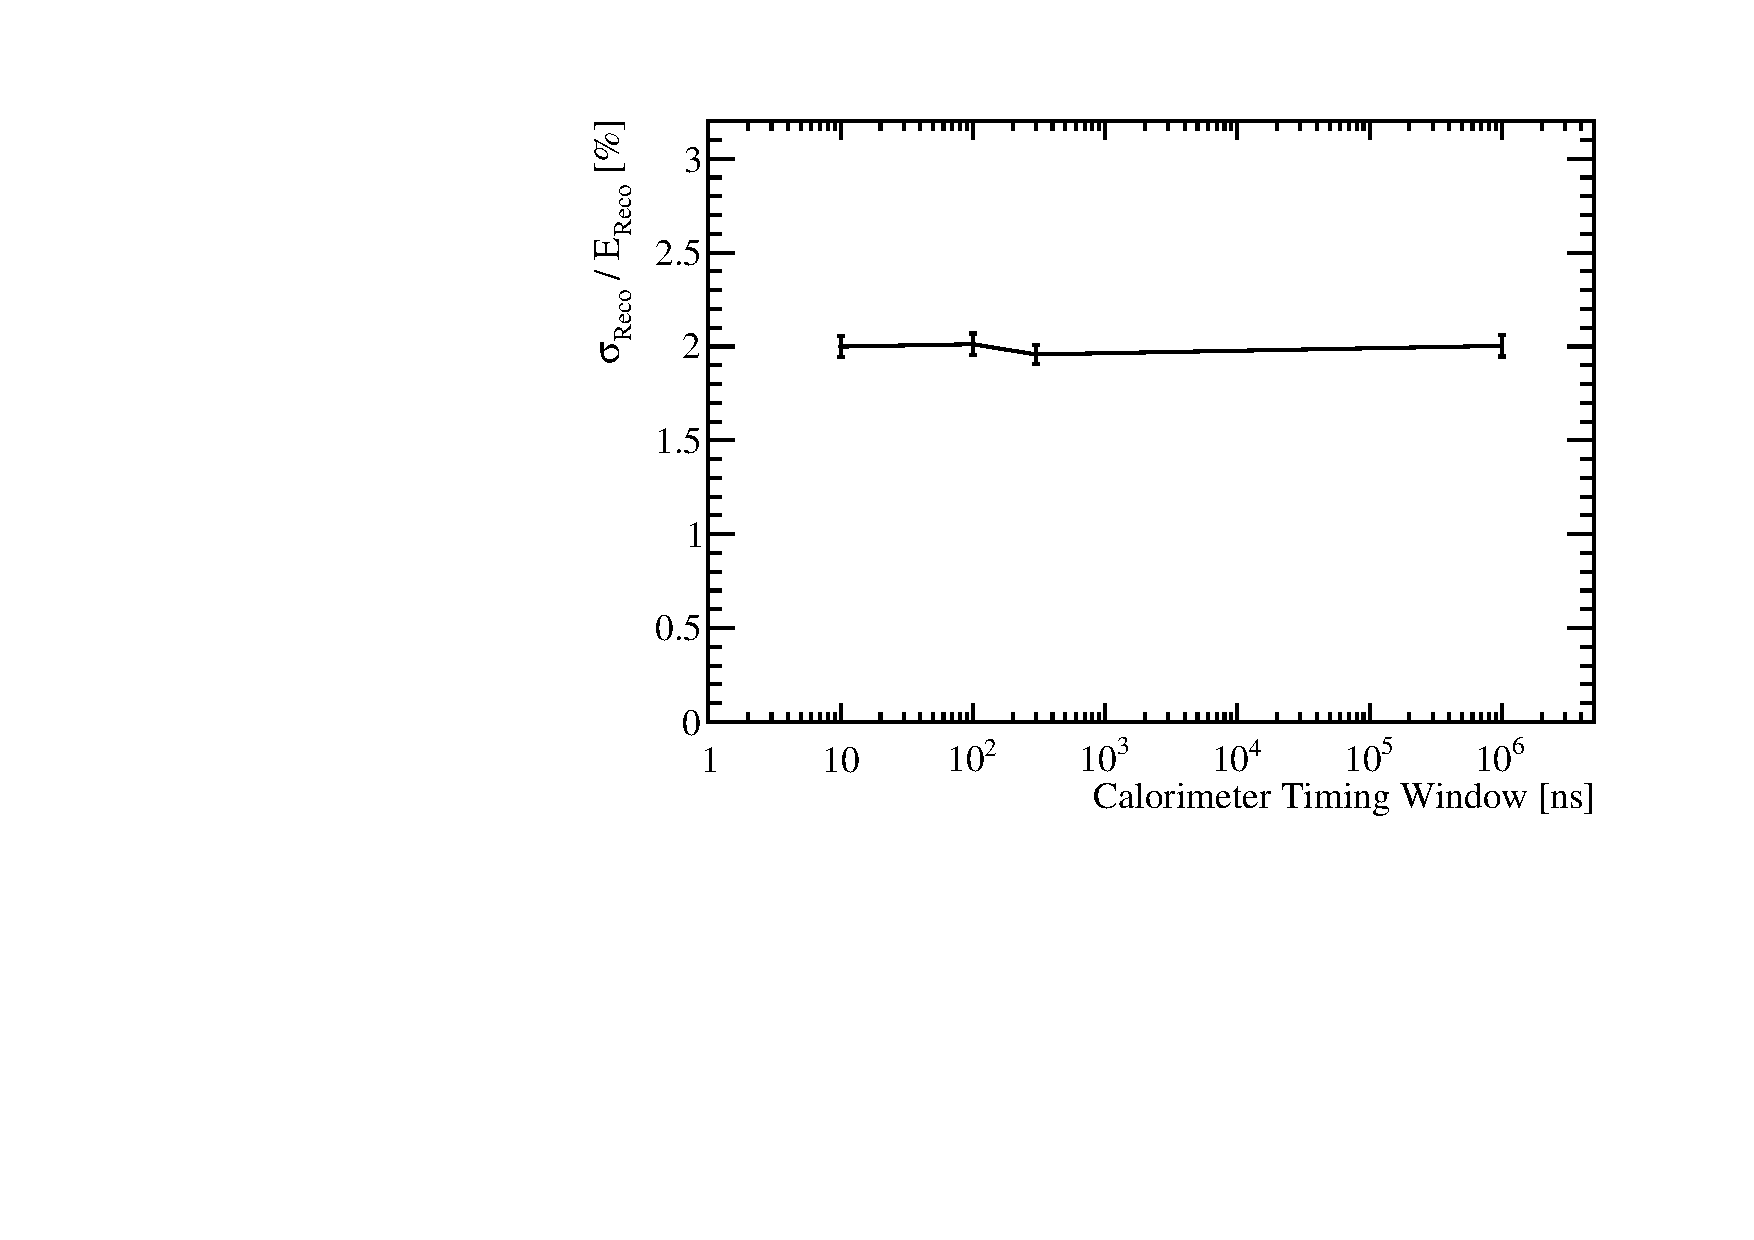
\includegraphics[width=0.5\textwidth]{EnergyEstimators/Plots/TimingCuts/ER_vs_PhotonTiming_100GeVPhoton.pdf}}
\subfloat[]{\label{fig:ertimingcutskaons}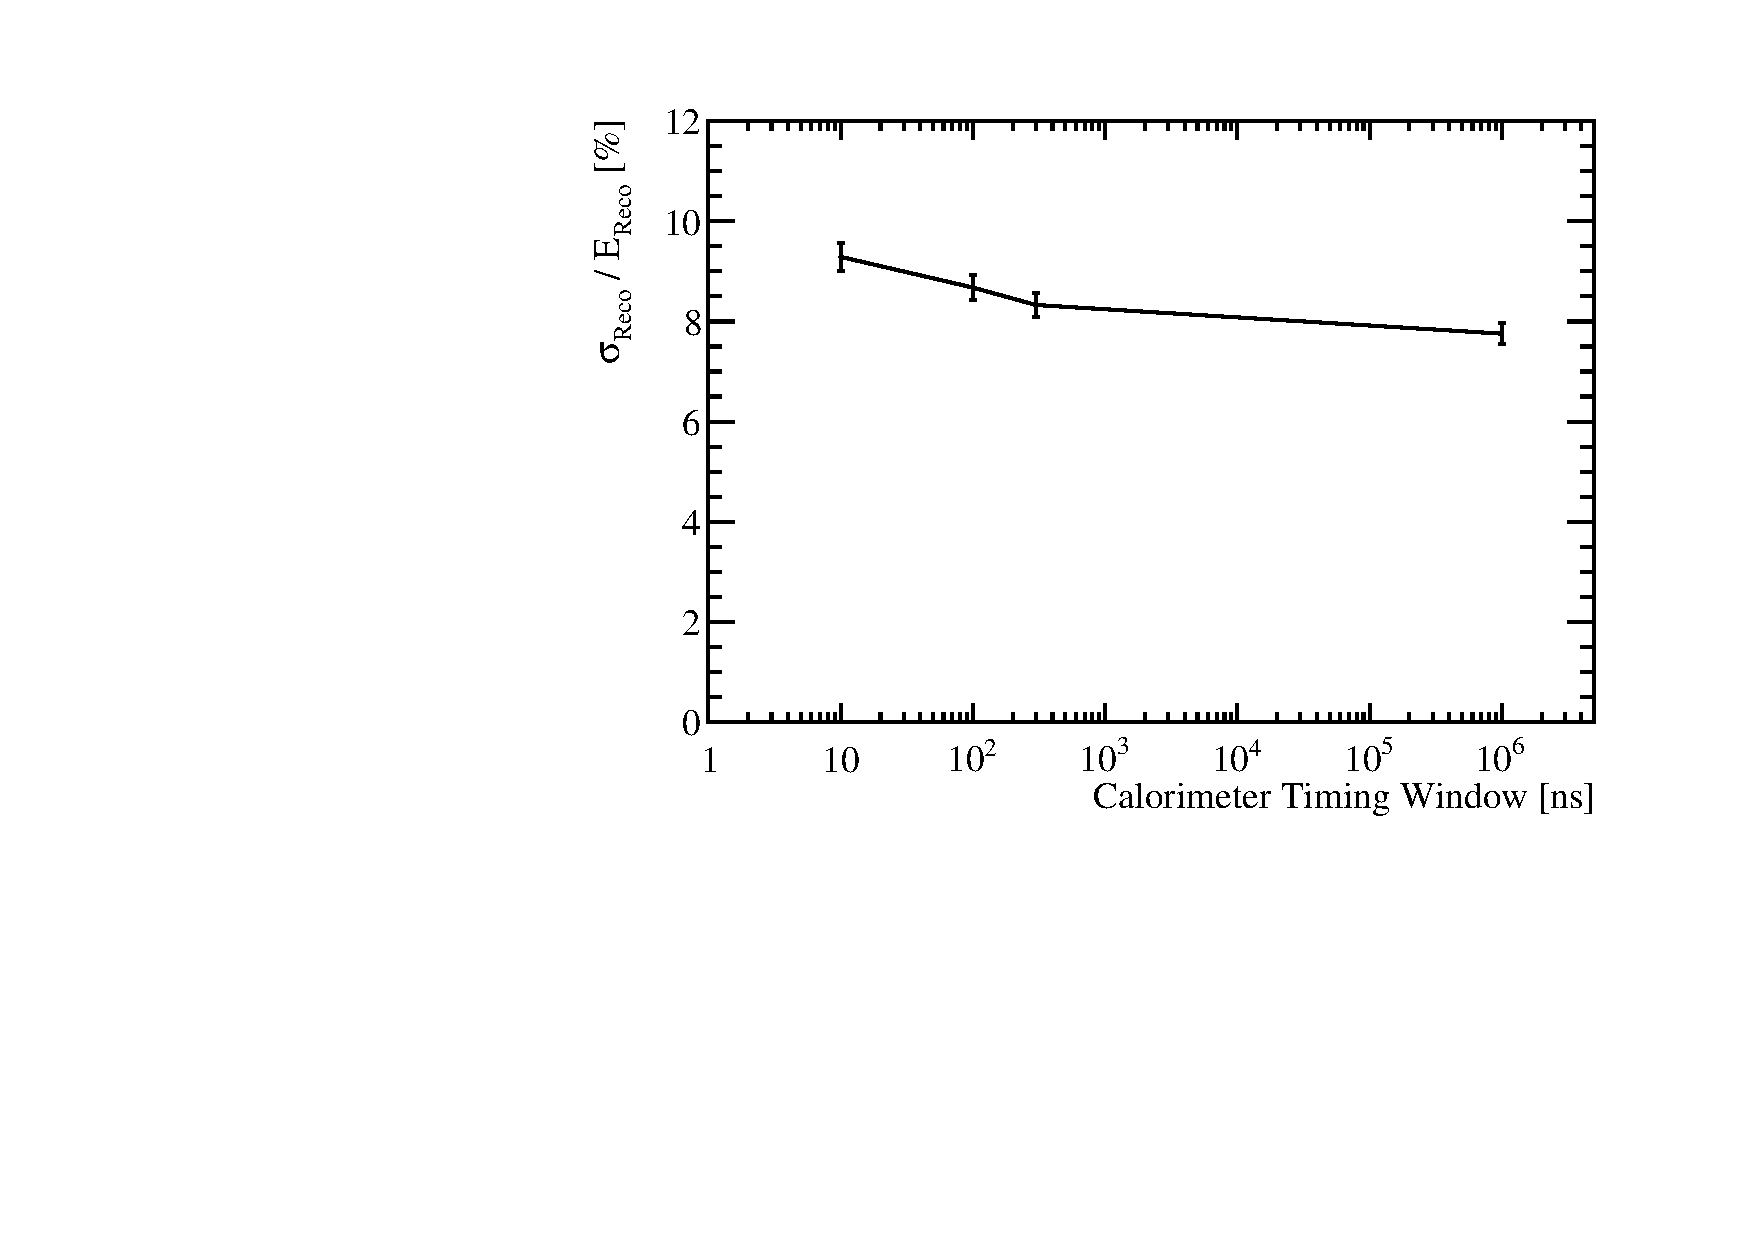
\includegraphics[width=0.5\textwidth]{EnergyEstimators/Plots/TimingCuts/ER_vs_Kaon0LTiming_50GeVKaon0L.pdf}}
\caption[The energy resolution as a function of calorimeter timing window for \protect\subref{fig:ertimingcutsphotons} 100 GeV $\gamma$ events and \protect\subref{fig:ertimingcutskaons} 50 GeV $K^{0}_{L}$ events using the nominal ILD detector model.]{The energy resolution as a function of calorimeter timing window for \protect\subref{fig:ertimingcutsphotons} 100 GeV $\gamma$ events and \protect\subref{fig:ertimingcutskaons} 50 GeV $K^{0}_{L}$ events using the nominal ILD detector model.}
\label{fig:ertimingcuts}
\end{figure}

\begin{figure}[h!]
\centering
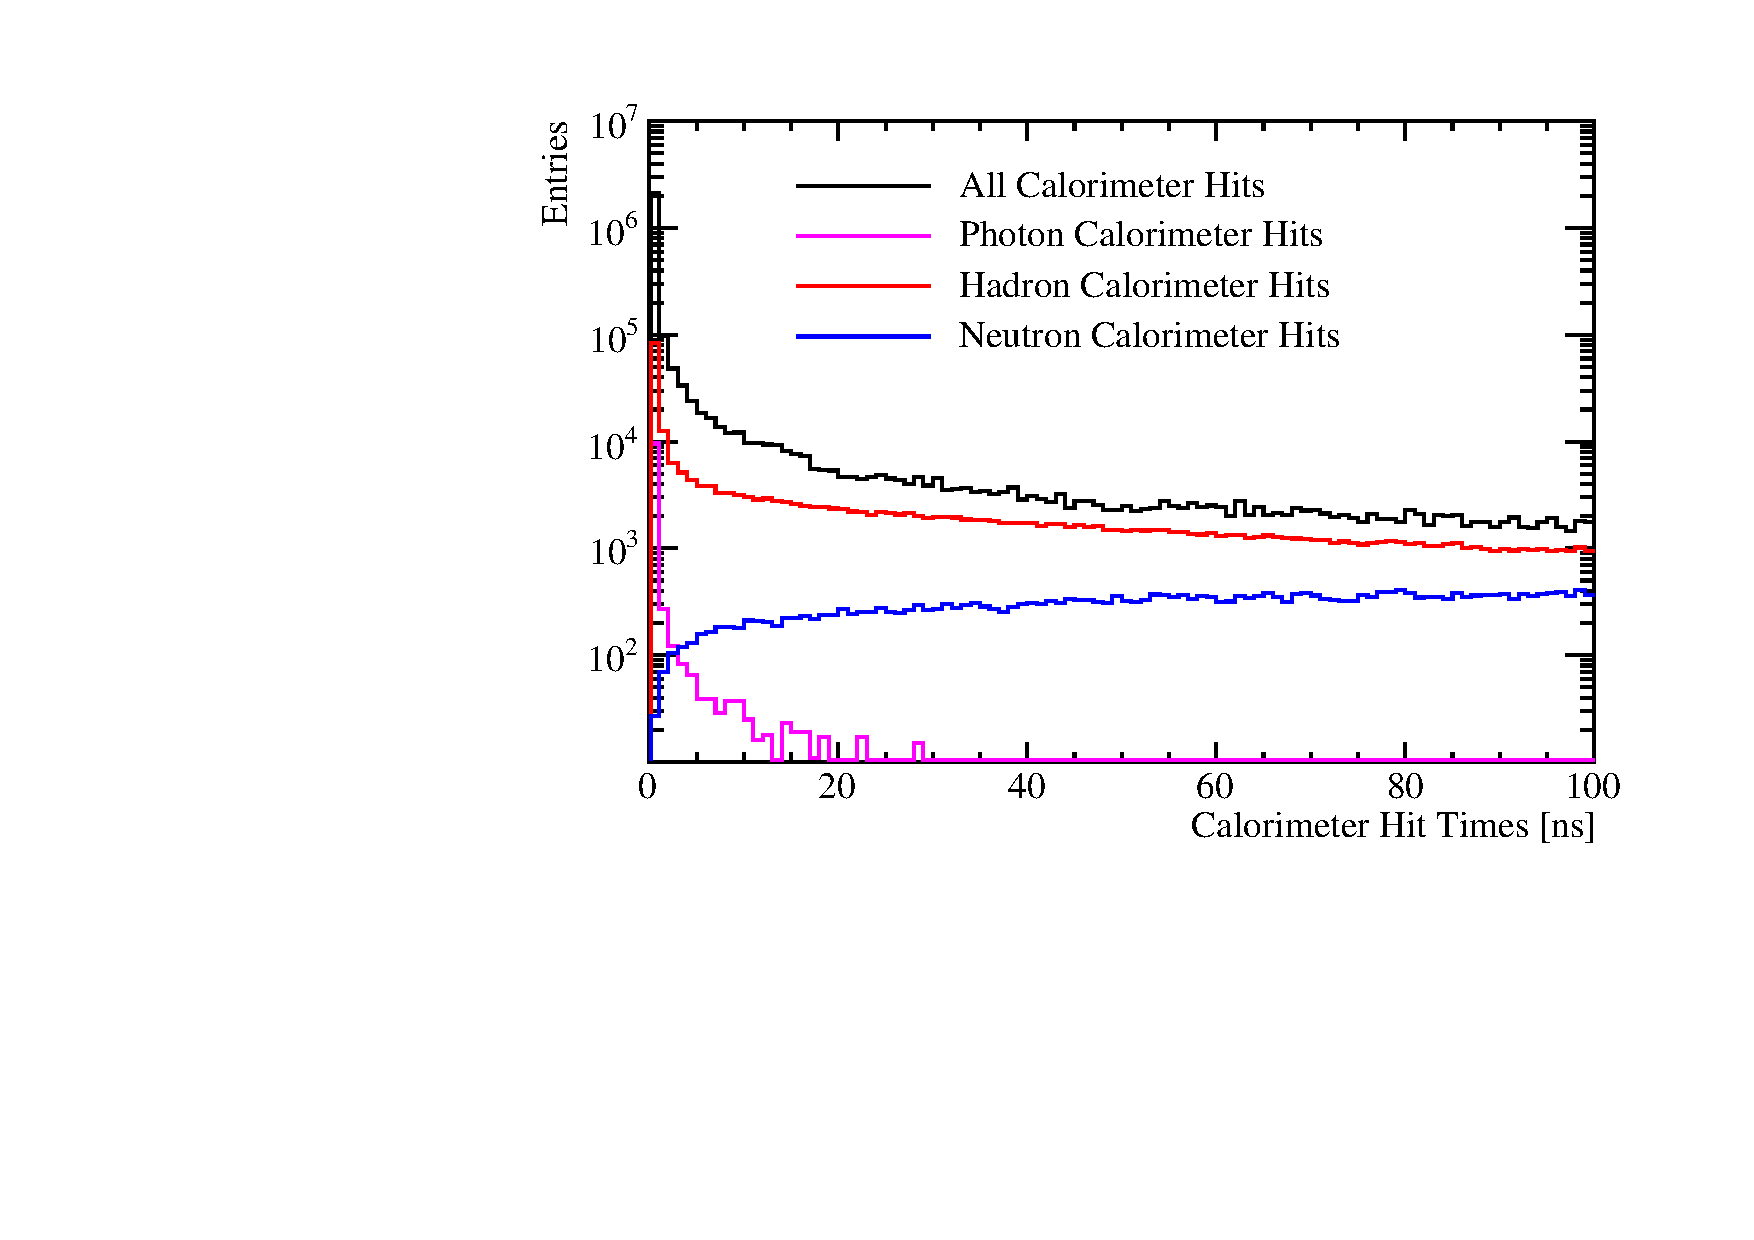
\includegraphics[width=0.5\textwidth]{OptimisationStudies/Plots/Description/CalorimeterHitTimes_91GeV_Z_uds_Steel.pdf}
\caption[The distribution of the time of the calorimeter hits, corrected for time of flight to the impact point, for 91 GeV Z$\rightarrow$uds di-jet events.]{The distribution of the time of the calorimeter hits, corrected for time of flight to the impact point, for 91 GeV Z$\rightarrow$uds di-jet events.}
\label{fig:calohittiming}
\end{figure} 

%========================================================================================

\subsubsection{Results: Jet Energy Resolution}
The jet energy resolution as a function of the jet energy for selected calorimeter time windows is shown in figure \ref{fig:jertimingcuts}.  As expected, the jet energy resolution will also be affected by the reduced neutral hadron energy resolution when the calorimeter timing window is reduced.  The sole exception to this is the 250~GeV jets for the 100~ns time window whereby the jet energy resolution is slightly better than when using the 300~ns and semi-infinite time windows.  As the magnitude of the changes to the jet energy resolution when varying the time window size are small in comparison to the absolute resolutions, this exception will most likely be due to a fluctuation in either the event sample used or in the reapplication of the calibration procedure.  

\begin{figure}[h!]
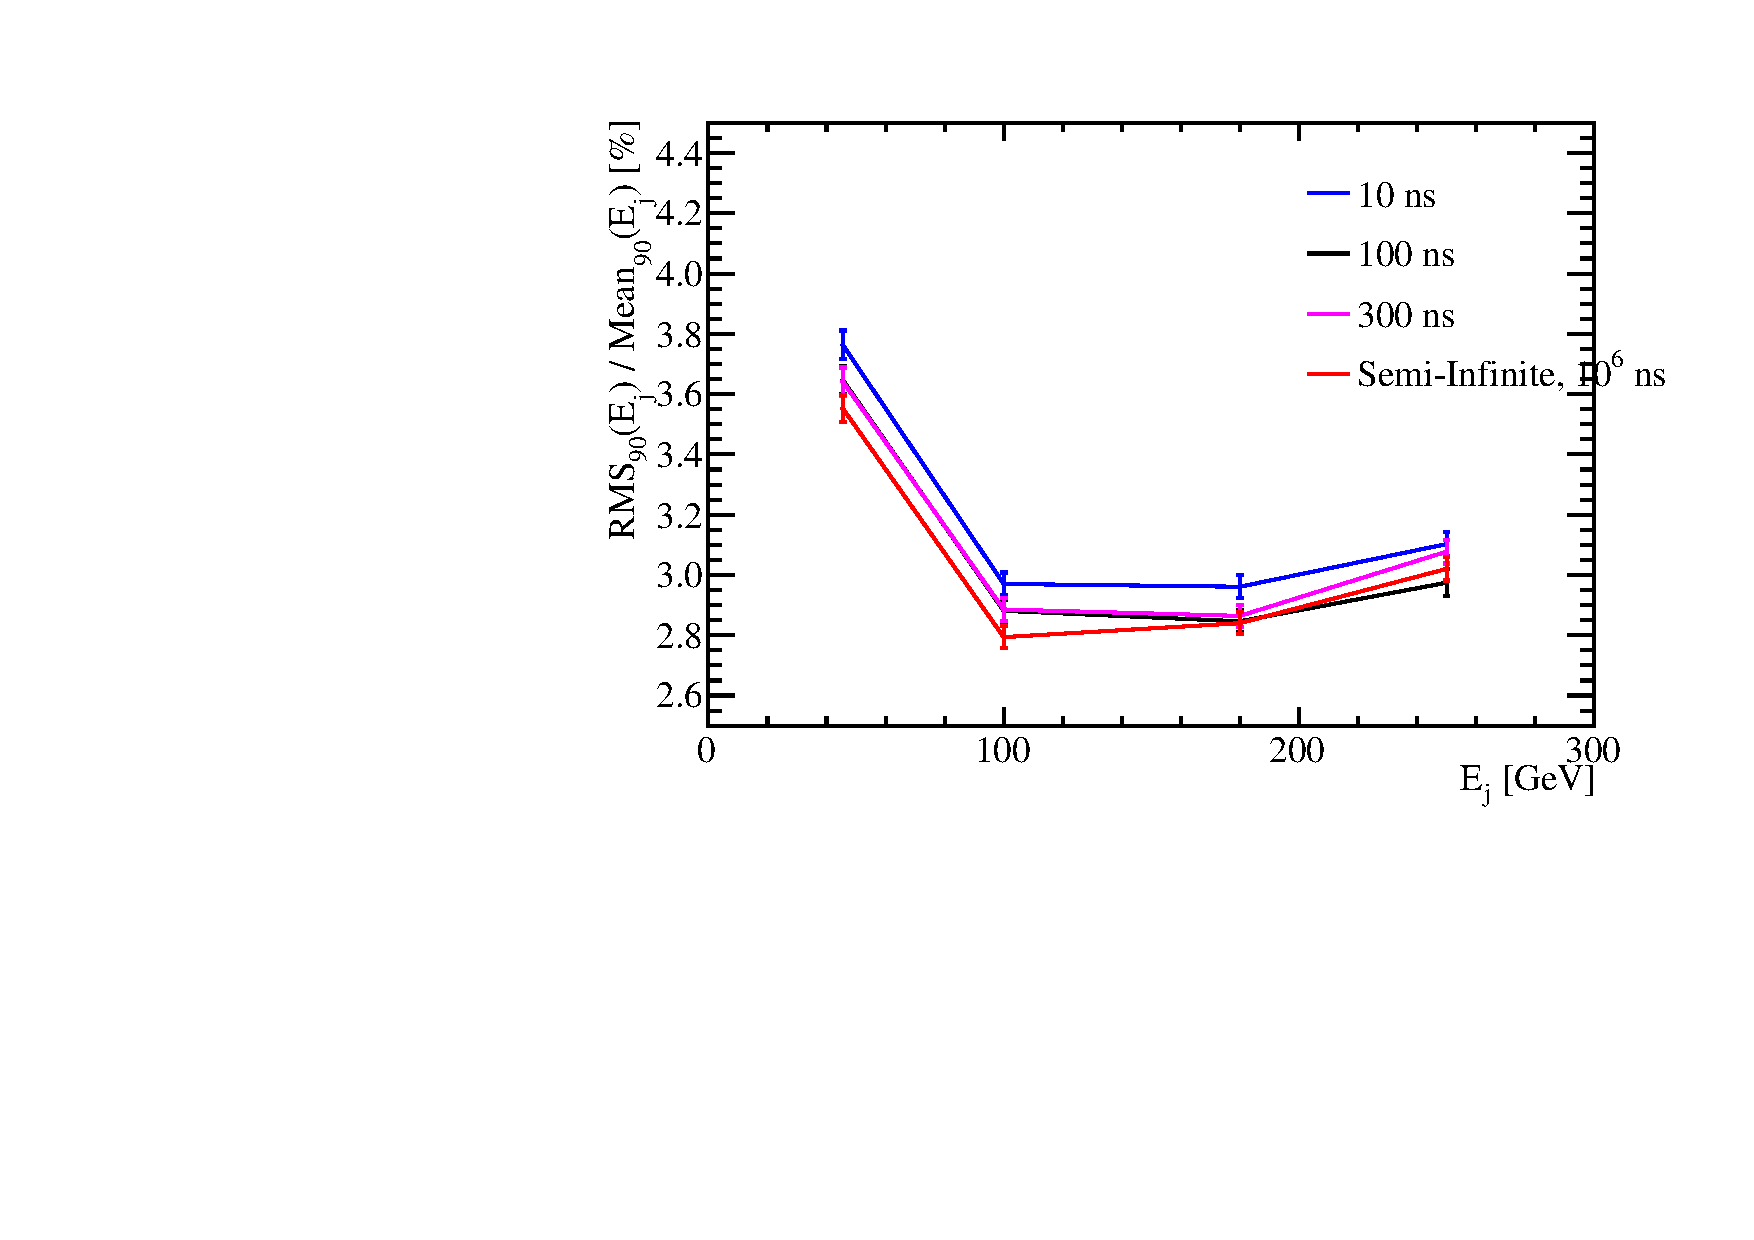
\includegraphics[width=0.5\textwidth]{EnergyEstimators/Plots/TimingCuts/JER_vs_JetEnergy_TimingCutStudies.pdf}
\caption[The jet energy resolution as a function of jet energy for various calorimeter timing cuts.  The results shown use the nominal ILD detector model.]{The jet energy resolution as a function of jet energy for various calorimeter timing cuts.  The nominal ILD detector model was used for this study.}
\label{fig:jertimingcuts}
\end{figure}

The time window applied to the calorimeter hits affects both the neutral hadron and jet energy resolutions with a larger timing window leading to better resolutions.  It can be seen that applying an aggressive choice of time window, such as 10~ns, the jet energy resolution is degraded as many of the hadronic showers being sampled do not have time to fully develop.  However, even using a 10~ns timing cut the jet energy resolutions are still sufficiently low to give excellent detector performance.  Both the single particle and jet energy resolutions indicate that the majority of hadronic showers will have fully developed within 100~ns and that there are little gains to be made by extending the size of this window.  

For results presented in this chapter and the optimisation studies found in chapter \ref{chap:detopt} a 100~ns timing window was applied across all models considered.  As the choice of timing window has yet to be finalised for the linear collider this value was chosen as it represents something that could be achieved using the readout technology options presently available \cite{Adloff:2014rya}.  Furthermore, it adds additional realism to the detector simulation in comparison to omitting the effect of the calorimeter time window.  The categorisation of changes to the detector performance when varying the calorimeter timing window presented here can be used to discern the impact of changing the timing window used for the optimisation studies at a later date if so desired.  

%========================================================================================
%========================================================================================
